\documentclass[12pt,table,xcdraw]{book}
\usepackage[a4paper,width=150mm,top=25mm,bottom=25mm,bindingoffset=6mm]{geometry}
\usepackage{fancyhdr}   
\usepackage{pbox}
\usepackage{dcolumn}
\usepackage{graphicx}
\usepackage{etoolbox}
\usepackage{pgf}
\usepackage{subcaption}
\usepackage{mwe}
\usepackage[utf8]{inputenc}
\usepackage[english]{babel}
\graphicspath{ {Images/} }
\usepackage[nodayofweek]{datetime}
\usepackage{natbib}
\usepackage{highlight}
\bibliographystyle{agsm}
\usepackage[normalem]{ulem} 
\useunder{\uline}{\ul}{}
%\usepackage[sectionbib]{chapterbib}
% \bibliographystyle{agsm}
\setcitestyle{authoryear,open={(},close={)}}
\usepackage{setspace}
\usepackage{url}
\usepackage{enumitem}
\usepackage{filecontents}
\usepackage{moresize}
\usepackage{minted}
\usepackage{pdflscape}
\usepackage[nottoc,notlof,notlot]{tocbibind} 
\usepackage{booktabs}
\usepackage{microtype}
\usepackage[document]{ragged2e}
\usepackage[font=small]{caption}
\usepackage{amsmath}
\usepackage{tcolorbox}
\usepackage{tabu}
\usepackage{longtable}
\usepackage{siunitx}
\usepackage{tabularx}
\usepackage{supertabular}
\usepackage{subcaption}
\usepackage{lscape}
\usepackage{float}
%\usepackage{unicode-math}
%\setmainfont{Latin Modern Roman}
%\setmathfont{Latin Modern Math}
\usepackage{relsize}
\usepackage{adjustbox}
\usepackage{rotating}
\usepackage{array}
\usepackage{multirow}
\usepackage{pifont}
\usepackage{tocloft}
\usepackage[justification=centering]{caption}
\usepackage{textcomp}
\usepackage{makecell}
\usepackage{hyperref}
\usepackage{cleveref}
\usepackage{pifont}
\usepackage[none]{hyphenat}
\usepackage[flushleft]{threeparttable}
\usepackage [autostyle, english = american]{csquotes}
\usepackage{color}
\usepackage{xcolor}

\newcommand*\OK{\ding{51}}
\newcolumntype{L}[1]{>{\raggedright\let\newline\\\arraybackslash\hspace{0pt}}m{#1}}
\newcolumntype{C}[1]{>{\centering\let\newline\\\arraybackslash\hspace{0pt}}m{#1}}
\newcolumntype{R}[1]{>{\raggedleft\let\newline\\\arraybackslash\hspace{0pt}}m{#1}}

\MakeOuterQuote{"}
\captionsetup{singlelinecheck=false}
\newcommand*\rot{\multicolumn{1}{R{90}{1em}}}

\newcommand{\specialcell}[2][c]{%
 \begin{tabular}[#1]{@{}c@{}}#2\end{tabular}}

\nocite{*} 
\renewcommand\cftsecleader{\cftdotfill{\cftdotsep}}

\setlength{\arrayrulewidth}{1mm}
\setlength{\tabcolsep}{18pt}
\renewcommand{\arraystretch}{1.5}

\setcounter{secnumdepth}{3}

% make neat dates
\renewcommand{\today}{\the\day \ \monthname \ \the\year}

% remove headers from book class
\fancyhf{}
\renewcommand\headrulewidth{0pt}
\fancyfoot[C]{\thepage}
\pagestyle{fancy}

\renewcommand{\bibname}{References}


\begin{document}
\frontmatter

\begin{titlepage}
\renewcommand{\today}{\monthname \ \the\year}
\begin{center}
\vspace*{1cm}

\Huge
\textbf{Tacit Knowledge Sharing in Open Innovation}\\
\vspace{1cm}

\Large
\textbf{Andrew Terhorst}
\vfill

\Large
A thesis submitted in total fulfilment\\
of the requirements for the Degree of \\
Doctor of Philosophy

\vspace{1cm}

\includegraphics[width=0.5\textwidth]{Images/swinburne_university_of_technology.png} 

\vspace{1cm}

\Large
Centre for Transformative Innovation\\
Faculty of Business and Law\\
\today
\end{center}
\end{titlepage}

\doublespacing

\addcontentsline{toc}{chapter}{Abstract}
\chapter*{Abstract}

A growing number of companies are turning to open innovation to stay competitive. Open innovation is formally defined as \textquote{a distributed innovation process involving the purposive management of knowledge flows across organisational boundaries using pecuniary and non-pecuniary mechanisms in line with the firm's business model} \citep{chesbrough2014explicating}. The innovation process relies heavily on accessing, absorbing, and harnessing knowledge across organisational boundaries with open innovation. Tacit knowledge refers to the knowledge, skills, and abilities an individual gains through experience that is difficult to put into words or otherwise communicate. It is strongly implicated in innovation as it guides the learning and thought processes that produce novel ideas. Despite the importance of tacit knowledge for innovation, it has received scant attention in the open innovation literature. \medskip

Open innovation implies extensive inter-organisational relationships to gain access to new external knowledge and exploit novel ideas. Proper understanding of open innovation processes requires a network rather than a firm-level perspective. This thesis treats an open innovation partnership as a temporary knowledge network deliberately set up to achieve a specific innovation outcome. It aims to improve our understanding of social mechanisms that enable or inhibit tacit knowledge sharing in open innovation by addressing four research questions: (1) What does the structure of tacit knowledge networks reveal about knowledge enacted in practice? (2) Does brokerage differ according to the type of knowledge exchanged? (3) To what extent does self-determination drive tacit knowledge sharing in open innovation? (4) What does the micro-structure of tacit knowledge networks reveal about trust and power relations in open innovation partnerships? Open innovation entails helping others develop the ability to apply knowing and knowledge in new and different contexts. Answers to these research questions should help people devise more effective strategies for bringing know-how and know-what together. \medskip

Sharing know-how is primarily an act of volition or free will. Hence, this thesis assumes human agency lies at the heart of tacit knowledge exchange. Finding the right balance between structure and agency is a challenge in open innovation. Too much structure may inhibit individual willingness to share tacit knowledge or contribute ideas. Conversely, too little structure can make goals less clear, leading to unsatisfactory open innovation outcomes. The academic literature suggests that human agents are primarily motivated to acquire tacit knowledge to satisfy an innate need for competence and gain sufficient power to maintain or enhance their autonomy, influence agendas, and enact change. External factors that affect tacit knowledge exchanges include subjective and behavioural norms, real or perceived boundaries, rules of engagement, and trust and power relations. The literature also suggests brokers have a crucial role in helping individuals overcome boundaries, build trust, and manage power relations. \medskip

This thesis used a combination of statistical social network analysis and semi-structured interviews to investigate the emergence of tacit knowledge network structures in three open innovation case studies. It used a critical realist approach to interpret quantitative and qualitative results. Most mixed-method studies embrace a pragmatic approach, where the goal is to obtain beneficial results, even though this involves alternating between paradigms. The stratified ontology of critical realism allows for the legitimate combination of qualitative and quantitative methods. A critical realist approach is particularly well-suited to a multiple case study approach where different contexts are in play. \medskip

The statistical social network analysis addressed observed or empirical reality. In contrast, the semi-structured interviews addressed unobserved or actual reality (the reality that shapes the emergence and functioning of knowledge provider networks). The statistical network analysis used exponential random graph models (ERGMs) to infer social processes in each case study's tacit and explicit knowledge provider networks. At the same time, the qualitative analysis of semi-structured interviews allowed a more profound exploration of the mechanisms and structures affecting tacit knowledge sharing. Applying the critical realist logic of retroduction and retrodiction to integrate the quantitative and qualitative results provided a more complete, expansive and diverse picture of the social mechanisms and structures affecting tacit knowledge sharing. \medskip

One set of ERGMs examined the role of motivation, trust, and power in tacit and explicit knowledge provider networks. Another set of ERGMs looked at broker roles in both the tacit and explicit knowledge provider networks. Results from the first set of ERGMs underscored the importance of tacit knowledge in open innovation. Path closure in a social network reflects a human tendency to form groups. Two of the partnerships had a significant path closure in their tacit knowledge networks. No such effect is evident in the explicit knowledge networks. In other words, tacit knowledge features strongly in group work. A significant receiver effect for autonomous motivation in each partnership's tacit knowledge network indicates that autonomous motivation is a reliable predictor of learning intent or knowledge-seeking behaviour. The second model runs indicate that path closure and broker roles can account for virtually all observed network configurations. Analysis of semi-structured interviews indicates that tacit knowledge is often under-valued, negatively impacting problem-solving and innovation. Moreover, the qualitative analysis indicates that brokers can profoundly affect the application of knowledge in practice. Tension was evident in those partnerships dominated by one individual. Trust features strongly in most decisions to share tacit knowledge. Perceived acts of self-interest erode trust and contribute to partner tension. Generally, people are less likely to disclose their hard-earned tacit knowledge in low-trust situations. \medskip

This thesis discovered that tacit knowledge resides in various internal and external communities of practice and that brokers are crucial for connecting these different communities. It confirmed that individuals are primarily motivated to seek out tacit knowledge to improve their level of self-determination. However, this thesis also found that close-minded individuals or individuals who consider themselves superior are less likely to connect with external communities of practice. The ability to tap external communities of practice is affected by several mechanisms, including actual or perceived boundaries and power and trust relations. This thesis also discovered that individuals are more likely to share their tacit knowledge if this delivers some personal benefit. It found that successful open innovation requires partners to invest in relationships to facilitate open and honest discussions vital for practical problem solving and innovation.

\addcontentsline{toc}{chapter}{Dedication}
\chapter*{Dedication}

This study is dedicated to my late parents. Without their support, I would never have been able to go to university and pursue an interesting career in research and development. I am sad they are not around to see me graduate as a Doctor of Philosophy. They would have been proud, I am sure.

\addcontentsline{toc}{chapter}{Declaration}
\chapter*{Declaration}

This doctoral thesis:

\begin{enumerate}
    \item Contains no material which has been accepted for the award to the candidate of any other degree or diploma, except where due reference is made in the text of the examinable outcome.
    \item To the best of the candidate’s knowledge contains no materials previously published or written by another person expect where due reference is made in the test of the examinable outcome.
    \item Where the work is based on joint research or publications, discloses the relative contributions of the respective workers or authors.
\end{enumerate} \bigskip

\includegraphics[width = 0.5\textwidth]{Images/Signature.png}\\
Andrew Terhorst\\
\shortdate{\today}

\addcontentsline{toc}{chapter}{Acknowledgements}
\chapter*{Acknowledgements}

This study was funded by the Commonwealth Scientific and Industrial Research Organisation (CSIRO) as part of its contribution to the Australian Research Council's Pathways to Market Industrial Transformation Hub hosted by the University of Tasmania. \medskip

\noindent
The author wishes to acknowledge the CSIRO for their extraordinary support and encouragement to get the job done. He is grateful to his supervisors, Professor Dean Lusher, Associate Professor Dianne Bolton, Dr Ian Elsum and Dr Peng Wang. This thesis would never have eventuated without their input. Associate Professor Dianne Bolton deserves special mention. Not only did she introduce the author to Professor Dean Lusher, but she was also always available to answer questions and offer advice. Dr Peng Wang went out of his way to extend \texttt{MPNet} to handle broker role parameters. This modification allowed the author to perform more realistic modelling of brokerage in his case studies. Thanks are due to Dr Aysha Fleming from the CSIRO for her helpful comments and encouragement. The author also wants to acknowledge fellow doctoral candidates, Bopha Roden and Sarah King, for their friendship and support. Karin Hosking checked the formatting, style, and accuracy of text in this manuscript. Ronald Burt (University of Chicago Booth School of Business), Henry Chesbrough (Haas School of Business at the University of California, Berkeley), and David Obstfeld (California State University) are thanked for sharing pre-publication material with the author. Garry Robins and Johan Koskinen from the University of Melbourne, and Carter Butts (University of California, Irvine) advised the author on various aspects of exponential random graph modelling. Last but not least, the author thanks the Swinburne University of Technology Higher Degree Research Office for helping him navigate the rules and procedures of doctoral studies. \medskip

\addcontentsline{toc}{chapter}{Foreword}
\chapter*{Foreword}

One must demonstrate a capacity for independent, critical thinking in a doctoral thesis. Examiners want to see evidence of originality and logical arguments. They do not want to see careless mistakes that indicate sloppy research \citep{mullins2002its}. My goal in writing this thesis was to present a rigorous and coherent analysis of tacit knowledge sharing in open innovation. It was clear early on that I would need a combination of quantitative and qualitative analysis to address my research questions. Reconciling different ontological and epistemological assumptions can be quite problematic in mixed-method research, which led me to embrace critical realism as my research philosophy. It allows one to consider reality in terms of observed or measured reality, perceived or unmeasured reality, and actual reality \citep{bhaskar2013realist}. Unpacking these different realities using deductive, inductive and retroductive reasoning has been eye-opening and confidence-building for me. \medskip

I knew very little about social network analysis at the beginning of my doctoral studies. Because social network analysis is data-intensive, I decided to learn how to program in \texttt{R} to become more proficient at data manipulation. I completed online data science courses offered by John Hopkins University (USA), namely \enquote{Computing for Data Analysis}, \enquote{Getting and Cleaning Data}, \enquote{Exploratory Data Analysis}, and \enquote{The Data Scientist's Toolbox}. Each course took 4 weeks to complete. Having mastered basic \texttt{R} programming, I then did an 8-week online course entitled \enquote{Social Network Analysis} offered by the University of Michigan (USA). This course provided an excellent foundation in social network analysis. To cap things off, I attended a 5-day \enquote{Introduction to Social Network Analysis} course offered by the Swinburne University of Technology. This course introduced me to exponential random graph models. I now consider myself a reasonably competent social network analyst. \medskip

I did not appreciate how much thought has to go into designing an online survey questionnaire until I completed an online course entitled \enquote{Questionnaire Design for Social Surveys} offered by the University of Maryland (USA). This 4-week course taught me to formulate short and unambiguous questions, avoid responder fatigue, manage selective recall, and pilot surveys. One component of this course addressed interviewing skills, which prompted me to explore further the theory and practice of successful interview techniques \citep[e.g.][]{kvale2008doing,seidman2012interviewing}. I also attended a one-day CSIRO course entitled \enquote{Human Research Ethics for Researchers}. This course introduced me to the \enquote{The National Statement on Ethical Conduct in Human Research}, which sets out national standards for the ethical design, review and conduct of human research. I made sure my research adhered to this standard. \medskip

I also completed a two-day introduction to \texttt{NVivo}\texttrademark\ course presented by QSR International as I planned to code semi-structured interview transcripts using this software package. Coding interview transcripts was particularly challenging for me. Everybody I spoke to approached coding differently. As \citet{saldana2015coding} notes, there is no right or wrong way to go about coding. After many false starts, I managed to find a way to code that allowed me to balance my thesis's quantitative and qualitative paradigms. Academic writing does not come easily to me. Early criticism of my writing was keenly felt. I only started to relax when it dawned upon me that I was becoming a \enquote{subject matter expert} and could communicate with some authority. \medskip

There is no doubt that I learned much about open innovation through my research. I discovered the importance of tacit knowledge for problem-solving and now understand how tacit knowledge defines who we are and what this means for power and trust relations. More importantly, I recognise the importance of skilled brokerage to facilitate tacit knowledge flows in open innovation. 

\newpage
\setcounter{tocdepth}{3}
\tableofcontents

\newpage

\listoffigures

\newpage

\listoftables

\mainmatter

\chapter{Introduction} \label{chp:intro}
% Introduction

\section{Scope of this study}

A growing number of Australian firms are turning towards open innovation as a competitive strategy. Not only does this allow them to access external knowledge resources, it also enables them to profit from internally developed knowledge by making it available to other firms. However, little is known about the role of tacit knowledge in open innovation. This is surprising considering tacit knowledge guides much of the learning and thought processes that produce novel ideas. This study attempts to fill this gap in understanding by examining tacit knowledge sharing in three open innovation projects. Particular attention is given to how people are motivated to share tacit knowledge and what different patterns of tacit knowledge brokerage reveal about power-relations in each case. \medskip

\section{Background}

\subsection{Need to innovate}

Much of Australia's prosperity stems from its natural advantages in agriculture and mining \citep{leung2016view}. Unfortunately, Australia is losing some of its comparative advantage\footnote{A country enjoys comparative advantage if it (a) can produce some set of goods at lower cost than a foreign country, and (b) is able to trade its relatively cheaper goods with relative cheaper goods produced by the foreign country} due to shrinking demand for it's mineral resources and increased regional competition. Australia can reverse this trend by becoming more innovative. Innovation can lead to the emergence of new industries that deliver long-term economic prosperity. \medskip

Innovation can be defined as the process of implementing new ideas to create value for an organisation \citep{schumpeter1950capitalism}. As long an idea is perceived as new by all those involved, it is an innovation even though it may appear to others as nothing more than an imitation of something that already exists elsewhere \citep{van1986central}. Failure to innovate places a firm’s ability to survive and prosper at risk \citep{bessant2005managing}. \medskip

Though Australia performs particularly well with respect to knowledge creation, it fares poorly when it comes to converting new knowledge into new-to-market innovations. Innovation does not feature strongly in the business strategies of established Australian firms \citep{dodgson2011systems,leung2016view}. This is reflected in the smattering of university-industry collaborations and low number of researchers employed in the business sector compared to other industrialised nations \citep{pettigrew2012australia}. Australia needs to become better at innovation if it wants to secure its long-term economic prosperity. \medskip

\subsection{Trend towards open innovation}

Firms are finding it is becoming harder to compete in the knowledge-based economy\footnote{The term \enquote{knowledge-based economy} refers to the increasing role of knowledge and technology in economic growth.}. Much of this can be attributed to the ever-increasing technical complexity of products, processes, and services that demand levels of knowledge beyond what most firms possess or can develop in a market-relevant time-frame. Many firms are turning towards open innovation to counter this \citep{enkel2009open,bessant2013innovation,stanko2017under}. \medskip

Open innovation is defined as a distributed innovation process based on carefully managed knowledge flows across firm boundaries, using mechanisms as per the firm's business model\footnote{The term \enquote{business model} refers to the design or architecture of the value creation, delivery, and capture mechanisms of a firm \citep{teece2010business}.}. The business model helps a firm determine which inflows of knowledge can fuel innovation, and which knowledge should be released to other organisations \citep{chesbrough2017future}. \medskip 

Key benefits of open innovation include early access to new technology, sharing of risk, reduced costs of development, better customer acceptance of products or services, and enhanced ability to continuously innovate \citep{ye2013exploring}. Because distributed innovation processes are hard to observe and thus imitate, open innovation is also a useful strategy for sustaining competitive advantage \citep{barney1991firm,lichtenthaler2011open}. \medskip

\subsection{Open innovation processes}

Open innovation can be described in terms of inbound, outbound and coupled innovation processes \citep{chesbrough2006beyond,enkel2009open,gassmann2010future}. \emph{Inbound open innovation} enriches a firm’s knowledge base through integrating suppliers, customers and other external actors \citep{xu2013inbound} whereas \emph{outbound open innovation} refers to the commercial exploitation of knowledge that has been developed in-house \citep{de2016knowledge}. \emph{Coupled open innovation} focuses on strategic partnerships that encompass both inbound and outbound innovation processes \citep{spithoven2013open}. Figure \ref{fig:oi_process} illustrates how these processes may work in practice. \medskip

\begin{figure}
	\centering
	\includegraphics[width=0.9\linewidth]{oi_process_2}
	\caption{Open innovation processes \citep{chesbrough2004open}. Image from SlideModel\texttrademark.}.
	\label{fig:oi_process}
\end{figure}

\subsection{Challenges of open innovation}

Despite its many potential benefits, open innovation presents considerable management challenges \citep{hossain2013open,vanhaverbeke2014surfing}. Overcoming relative differences in absorptive capacity between open innovation partners is a particularly difficult challenge \citep{vanhaverbeke2007connecting,lakemond2016match}. Absorptive capacity refers to the \enquote{ability of a firm to recognise the value of new, external information, assimilate it, and apply it to commercial ends} \citep{cohen1990absorptive}. Firms need absorptive capacity to make sense of new external knowledge and allow them to capture value from open innovation processes \citep{vanhaverbeke2007connecting}. Relative differences in absorptive capacity can impede the flow of knowledge across organisational boundaries, contribute to power imbalances, and undermine alliance performance, all of which can result in sub-optimal open innovation outcomes \citep{szulanski1996exploring,lane1998relative,nooteboom2000learning,vanhaverbeke2007connecting,easterby2008absorptive,phelps2012knowledge}.\medskip 

\subsubsection{Mobilising tacit knowledge}

Past studies of absorptive capacity emphasise the importance of prior knowledge possessed by individuals and groups. The knowledge resource available to a firm can be likened to an iceberg. Explicit knowledge is the visible tip of the iceberg, easy to recognise and access. Hidden beneath the surface of conscious thought, is the vast bulk of the iceberg, symbolising tacit knowledge derived from years of experience, practice, perception, and learning \citep{spender1996making,haldin2000difficulties,mcadam2007exploring,rebernik2007fostering}. Tacit knowledge is associated with terms such as \enquote{intuition}, \enquote{skill}, \enquote{know-how}, and \enquote{expertise} used to describe knowledge that refers to an ability to perform work \citep{horvath2000working,mcadam2007exploring}. Much of the prior knowledge possessed by individuals and groups is likely to be tacit in nature. \medskip

The most common application of tacit knowledge is problem-solving. People with expertise borne from experience not only are able to recognise the situation in which they find themselves in, but also know which actions might be appropriate for dealing with it \citep{simon1971human,leonard1998role}. Tacit knowledge can also used to re-frame problems or anticipate outcomes in intuitive ways \citep{leonard1998role}. Because tacit knowledge guides the thinking that produces novel ideas, it is critical for innovation \citep{leonard1998role,amar2008descriptive}. \medskip

Mobilising tacit knowledge is particularly challenging because people are either unaware of the tacit dimension of their knowledge or unable to express what they know \citep{polanyi1966tacit,leonard1998role}. Many firms do not appreciate the diversity of their knowledge resource and lack processes to unlock the potential value of tacit knowledge \citep{nonaka1994dynamic,horvath2000working}. Sharing tacit knowledge is also something that cannot be mandated. It mostly happens through volition or free will \citep{polanyi1966tacit}. Some people may also be reluctant to give up any advantages their tacit knowledge or know-how affords them \citep{eraut2000non}. \medskip

Tacit knowledge is not transferred but rather interpreted within a specific context \citep{nonaka1995knowledge,duguid2005art,marabelli2014knowing}. Face-to-face social interaction is considered the richest medium because it allows immediate feedback to check understanding and correct interpretations \citep{koskinen2003tacit}. \medskip

\subsubsection{Brokering productive relationships}

Boundary spanners play a key role in open innovation as they broker new relations between otherwise disconnected actors in different organisational networks. More importantly, they facilitate the translation, integration and combination of unfamiliar and distant knowledge \citep{granovetter1973strength,tushman1981boundary,allen1984managing,szulanski2003sticky,burt2004structural,burt2007secondhand,seidler2008use,meyer2010rise,chesbrough2012open}. \medskip

Management efforts to create or widen existing inter-organisational networks may be frustrated by people reluctant to form new ties, facilitate third-party ties, or otherwise change their existing networks \citep{davis2010agency}. Negative attitudes such as \enquote{not-invented-here} and \enquote{not-shared-here} (also referred to as \enquote{not-sold-here}) syndromes can stymie knowledge exchange \citep{lichtenthaler2006attitudes,lichtenthaler2011your,de2014neither,podmetina2015skills,chesbrough2017future}. Not-invented-here syndrome refers to resistance within a firm against externally developed knowledge \citep{katz1982investigating,hussinger2011search,antons2015opening}. Not-shared-here syndrome is a negative attitude towards external exploitation of internally developed knowledge \citep{chesbrough2003open,lichtenthaler2006attitudes,de2014neither}. \medskip

Figuring out ways to overcome negative attitudes towards knowledge sharing is essential to allow the formation of new productive relationships that enable knowledge to be recombined in unique and valuable ways \citep{uzzi1997social,nahapiet1998social,obstfeld2005social,lane2006reification,davis2010agency,meyer2010rise}.\medskip

\section{Research opportunity}

\subsection{Exploring motivational factors}

Tacit knowledge requires significantly more effort than explicit knowledge to communicate. People need to be sufficiently motivated to seek out and share tacit knowledge \citep{leonard1998role}. Past studies show a significant and positive relation between an individual's level of intrinsic motivation and the amount of tacit knowledge they share  \citep[e.g.][]{osterloh2000motivation,kaser2001knowledge,smith2001role}. Intrinsic motivation is about engaging in activity because it is enjoyable or personally meaningful \citep{ryan2000intrinsic}. Although these studies highlight the importance of personal motivation, the psycho-social processes underpinning tacit knowledge sharing and how this impacts open innovation are not well understood. This indicates a need to investigate how personal motivation shapes the development of knowledge sharing relations. \medskip

\subsubsection{Unpacking power-relations}

Though it is often stated that \enquote{knowledge is power}, little attention has been  to power and power-relations in the knowledge management literature \citep{heizmann2015power}. The current power literature is dominated by two contrasting views of power, namely \enquote{power as domination}, also referred to as \enquote{power-over}, and \enquote{power as empowerment}, often characterised as \enquote{power-to} \citep{haugaard2012rethinking}. Sharing tacit knowledge is about empowering others so they can perform work more independently and confidently \citep{bordum2002tacit,lin2007share}. \medskip

The network perspective treats power as inherently relational \citep{ibarra1993network}. How an actor is embedded in a social network either imposes constraints on the actor or presents them with opportunities \citep{burt1992structural,simpson2011network}. Actors with fewer constraints and more opportunities occupy favourable structural positions. Being in a favoured position means that an actor may extract better bargains in exchanges, have greater influence, and be a focus for deference and attention from those in less favoured positions \citep{burt1992structural,hanneman2005introduction,simpson2011network}. \medskip

Actors in knowledge networks serve both as keepers of knowledge and as agents that seek out, communicate, and create knowledge \citep{phelps2012knowledge}. One can assess how actors exercise power by examining patterns of brokerage in knowledge sharing networks. Brokerage may be defined as the \enquote{behaviour by which an actor influences, manages, or facilitates interactions between other actors} \citep{obstfeld2014brokerage}. This definition allows brokerage to be seen in terms of \enquote{power-over} and \enquote{power-to}. \medskip
 
\section{Study objectives}

The extent to which tacit knowledge helps bridge cognitive gaps is poorly understood. Research into brokerage of tacit knowledge is also lacking. This is not surprising, given tacit knowledge is difficult to characterise let alone measure \citep{zander1995knowledge,cavusgil2003tacit}. Tacit knowledge has a significant influence on a firm's absorptive and innovative capacity, and warrants much more attention than it has received so far. \medskip

This study explores tacit knowledge sharing in three open innovation partnerships. Attention is focused on how people are motivated to share tacit knowledge and how tacit knowledge is brokered in each partnership. Four research questions are addressed in this study: \medskip

\begin{description}
    \begin{enumerate}
        \item To what extent does the level and type of personal motivation predict tacit knowledge sharing in open innovation partnerships?
	    \item What does the configuration of tacit knowledge networks reveal about power-relations in open innovation partnerships?
	    \item What is the relationship between tacit knowledge sharing and idea generation in open innovation partnerships?
	   \item How does organisational culture contribute to tacit knowledge sharing in open innovation partnerships
    \end{enumerate}
\end{description}

The study employs social network analysis to (a) assess how individual attributes, such as level and type of personal motivation, educational background, and work experience drive the emergence of tacit knowledge sharing relations, and (b) examine what patterns of brokerage reveal about power-relations in tacit knowledge networks. This analysis is complemented by semi-structured interviews that capture the industrial, organisational, and cultural contexts governing the emergence of collaborative social structures. \medskip  

\section{Research contribution}

This study advances knowledge in two ways. Firstly, the study provides fresh insight into how tacit knowledge sharing facilitates learning and idea generation in open innovation partnerships. Secondly, it breaks new ground by examining how brokerage roles vary according to the amount of tacit knowledge being exchanged and what this means in terms of power-relations. Both contributions should contribute to more effective management of tacit knowledge flows in open innovation. \medskip

\section{Document structure}

This document is organised into nine chapters:

\begin{itemize}[leftmargin=0pt]
  \item[] \textbf{Chapter two} explores the concept of tacit knowledge and reviews key psychological and social theories that may be used to assess knowledge sharing behaviour. These include the theory of planned behaviour, self-determination theory, structural hole theory, and brokerage theory. The chapter presents a number of propositions that inform the subsequent analysis.
  
  \item[] \textbf{Chapter three} provides an overview of social networks and social network analysis. The reader is introduced to exponential random graph models, an advanced type of social network analysis used in this study.
  
  \item[] \textbf{Chapter four} describes the research methodology underpinning this study. This includes explaining the rationale for the convergent parallel mixed method research design used in this study and detailing the quantitative and qualitative procedures used to collect and analyse data.
  
  \item[] \textbf{Chapter five} summarises key characteristics of each open innovation case. This includes a description of the innovation challenge being tackled, information about each partner organisation and the individual actors involved, and a statement on how much progress has been achieved at the time of data collection.
  
  \item[] \textbf{Chapter six} reports on how individual attributes such as level of personal motivation, education level, work location, and job experience shape tacit knowledge sharing relations in each open innovation partnership.
  
  \item[] \textbf{Chapter seven} discusses the different patterns of knowledge brokerage encountered in each partnership and what these reveal about nature power-relations using information from both the social network analysis and semi-structured interviews.
  
  \item[] \textbf{Chapter eight} discusses the implications for managing tacit knowledge flows in open innovation partnerships. 
  
  \item[] \textbf{Chapter nine} summarises the main findings of this study and reflects on some key lessons learned as this study unfolded. This includes describing study limitations and possible avenues for future research. 
\end{itemize}

\chapter{Literature review} \label{chp:lit_review}
% Chapter 2 - Social network perspective
\section{Introduction}

Firms access knowledge, resources, markets, or technologies via various social networks \citep{inkpen2005social}. The span of an organisation’s network of ties to partners (reach) and the resources that the organisation can access via its partners (richness) determine the value that it can potentially extract from its inter-organisational networks \citep{gulati2011networks}. Reach and richness bring together structural and relational properties that, together with associated organisational capabilities, explain the performance implications of networks in an integrated manner. The configuration of a firm's network ties determines how easily knowledge can be transformed into valuable innovations \citep{tortoriello2010activating}. We can use social network analysis to examine network configurations and determine the extent to which these are shaped by individual attributes and knowledge properties. This chapter describes some of the salient features of social networks and key social mechanisms for mobilising knowledge. It then introduces exponential random graph models, an advanced social network analysis technique for examining network configurations. \medskip  

\section{Social networks}

Social networks provide a way of thinking about social systems, one that focuses on the relationships among entities that make up the system \citep{borgatti2013analyzing,robins2015doing}. Networks can be represented mathematically as graphs consisting of a set of vertices and a set of edges that connect vertices \citep{newman2010networks}. \medskip

Vertices represent actors or nodes in a social network, which can be individuals, groups, organisations, regions, or even nations. Actors may be distinguished by binary, categorical or continuous attributes. For example, consider an individual actor classified as female (binary attribute), who works for a particular organisation (categorical attribute), with a specific number of years work experience (continuous attribute). \medskip

Edges represent relations or social ties between actors. Ties can be measured as directed or undirected and as binary or valued. Deciding whether to measure a tie as directed or undirected depends on the theoretical nature of the tie. For instance, co-membership is inherently undirected whereas authority is essentially directed. Directed and undirected ties can be measured as binary ties that either exist or do not exist, or as valued ties that can be stronger or weaker, transmit more or fewer resources, or have greater or lesser amount of contact \citep{scott2011sage}.\medskip

Different types of relations may exist between actors with each type of relation giving rise to a corresponding network \citep{borgatti2013analyzing}. Measuring knowledge sharing ties would, for example, generate a knowledge sharing network. Assigning an attribute to the knowledge sharing tie allows us to qualify the relationship in terms of, say, the content or frequency of knowledge sharing (e.g. how much of the knowledge be shared is tacit in nature). \medskip

Figure \ref{fig:tie_type} characterises different types of social ties. Ties between actors who share something in common (e.g. work at the same location, are affiliated to the same body, participate in the same event, or share a common attribute) are referred to as similarity ties. Relational ties include kinship and other ties, such as friendship, advice, and managerial ties. Relational cognition refers to ties that are affective (e.g. like or dislike another actor) or perceptual (e.g. belief about the other actor) in nature. Relational events refer to ties defined by specific social interactions (e.g. a transaction of some kind) and flows (e.g. knowledge flows). \medskip

\begin{figure}
	\centering
	\includegraphics[width=0.9\linewidth]{tie_type}
	\caption{Different types of ties. Modified after \citet{borgatti2009network}.}
	\label{fig:tie_type}
\end{figure}

Actors who know each other well are said to have strong ties with one another. Ties that are characterised by infrequent interaction, short histories, and limited emotional closeness may be characterised as weak ties \citep{baer2010strength}. Some ties are dependent on others. An example is friendship, which usually develops because of an pre-existing similarity tie (e.g. both actors live in the same neighbourhood, attend the same school, or work at the same place) or via a relational event tie (e.g. actors were introduced to each other at a specific event or worked together on a particular project). Actors are more likely to share knowledge (relational event) with others who have common interests (similarity tie) or with others they trust (relational cognition). Multiplex relations between two actors are considered to be stronger because their redundancy can make them endure the rupture of a specific type of connection \citep{dickison2016multilayer}. \medskip 

\section{Social network analysis}

The aim of social network analysis is detecting and interpreting patterns of social ties between actors \citep{wasserman1994social,de2011exploratory}. Most basic questions in social network analysis involve the measurement and modelling of particular structural properties such as reciprocity, degree distribution, triadic closure, and homophily \citep{butts2008social,snijders2011statistical}. To fully understand the implications of dyadic relations between actors, one has to consider how these are shaped by broader patterns of social interaction \citep{scott2011sage}. This requires more than simply measuring the basic characteristics of networks. A set of assumptions is needed to best describe and explain social phenomena of interest. This may involve applying an existing psychological or social theory to develop propositions or test hypotheses about specific social relations \citep{scott2011sage,borgatti2013analyzing}. \medskip

Actors in knowledge networks serve both as keepers of knowledge and as agents that seek out, communicate, and create knowledge \citep{phelps2012knowledge,pugh2013designing}. Knowledge by itself is simply a latent resource. It only becomes valuable once it is mobilised and used \citep{marabelli2012knowledge,freeman2015knowledge}. Examining the local configuration of knowledge networks can shed light on the social processes that transform new knowledge into innovations. \medskip

For instance, actors that know each other well are said to have strong ties with one another. Such actors tend to have similar interests and are privy to the same knowledge. Strong ties tend to make people look inward and not be very receptive to external knowledge. Casual acquaintances, on the other hand, can be regarded as weak ties. Because acquaintances usually mix in different social circles, weak ties are more likely to provide actors access to new knowledge and opportunities \citep{granovetter1973strength}. \medskip

Knowledge networks with an abundance of weak ties are typically sparse with many disconnected parts or \enquote{structural holes} \citep{burt1992structural}. Actors who bridge otherwise disconnected parts of the knowledge network are termed knowledge brokers. Brokerage may be defined as the \enquote{behaviour by which an actor influences, manages, or facilitates interactions between other actors} \citep{obstfeld2014brokerage}. Knowledge brokers make connections between those who need knowledge and those who have it \citep{davenport1998successful}. They are able to identify and establish strategic relationships with keepers of knowledge. Some knowledge brokers exploit this to their own advantage while others try establish new relations between otherwise disconnected people \citep{gould1989structures,burt1992structural,obstfeld2014brokerage}. One can assess how actors exercise power by examining patterns of brokerage in knowledge sharing networks. \medskip

Reciprocity is a key concept in social exchange and game theory that reflects a human tendency to return helpful or harmful acts in kind \citep{nowak2005evolution}. Both social exchange and game theory suggest dyadic relationships have a tendency to be symmetrical \citep{emerson1976social,axelrod1984evolution}. In other words, reciprocity leads to balanced and more stable relations, which in turn helps build trust and strengthen ties between actors \citep{blau1964exchange}. Non-reciprocated or asymmetric ties are more likely to be unstable i.e. are unlikely to be long-lasting or strong \citep{snijders2011statistical}. \medskip %Past studies show that people are more inclined to share knowledge with others if this behaviour is reciprocated \citep{ipe2003knowledge}. \medskip

Past studies show that when new actors join a social network, there is an attachment bias i.e. actors are more likely to connect with other actors who are already quite popular. This is also referred to as \enquote{preferential attachment} \citep{barabasi1999emergence}. The implication of such a bias is that well-connected actors will increase their connectivity at a higher rate than less well-connected actors, the so-called \enquote{rich-get-richer} phenomenon \citep{desollaprice976general}. In other words, preferential attachment suggests that some people in a knowledge exchange network will acquire knowledge at a faster rate than others. Given that knowledge is a source of power, this has implications for power-dependence relations. More central actors are able to exert much more influence because they have greater access to diverse knowledge \citep{emerson1962power,bonacich1987power}. \medksip 

Sociologists are particularly interested in group processes and how these impact individual perceptions and behaviour \citep{de2011exploratory}. Balance theory argues people feel uncomfortable when they think their friends do not like each other \citep{heider1958psychology}. To resolve this discomfort, the theory predicts that one will either discard a friend, or more likely, one will change one’s perceptions of the relationship between friends to restore cognitive balance i.e. \enquote{a friend of a friend is a friend of mine} \citep{krackhardt1987cognitive}. Achieving structural balance in social relations typically results in triadic or transitive closure, which can be either cyclic or hierarchical in nature. Cyclic closure tends to relatively low in social networks, indicating the pervasiveness of hierarchies in local group structures \citep{davis1967structure}. \medskip  

Homophily is the tendency of similar actors to relate to each other \citep{mcpherson2001birds}. Theoretical arguments can be based on opportunity, affinity, ease of communication, reduced transaction costs and break-off risks, and organisational foci composed of similar individuals. This leads to a higher probability of ties being formed between actors with similar values on relevant covariates \citep{snijders2011statistical}. \medskip

\section{Exponential random graph models}

Exponential random graph models (ERGMs) are a class of statistical model for social networks originally developed by \citet{frank1986markov} and refined by \citet{wasserman1996logit} and \citet{pattison1999logit}. ERGMs have the capacity to address complex social structures. Recent model derivations are able to examine both individual-level variables and structural relations simultaneously \citep{robins2007recent}. \medskip

An ERGM is essentially a pattern recognition device which breaks a network down into its constituent network motifs or configurations and then test if particular configurations occur more or less frequently than would be expected by chance alone. Network configurations are patterns of social network ties assumed to represent underlying social processes or mechanisms \citep{lusher2014cooperative}. For example, a theory may suggest that actors with specific attributes are more likely to receive social ties. This can be tested using an ERGM to see if actors with such attributes are receiving more ties than would be expected by chance alone. That way, a researcher can test certain hypotheses or propositions about tie formation relating to theory \citep{robins2007recent}. \medskip

ERGMs permit differentiation between structural network effects and processes related to actor attributes. Unlike the assumption of independence of observations in standard statistical tests, ERGMs are based on the assumption of conditional dependence \citep{pattison2002neighborhood}. An ERGM is similar to a logistic regression, but is more sophisticated because it can handle complex dependency assumptions. This reflects social reality where ties are largely interdependent \citep{kadushin2012understanding}. \medskip

Purely structural effects reflect self-organising or endogenous processes in which ties form due to the presence or absence of other ties. In the case of reciprocity, for example, because one person has first done someone a favour, that other person is more likely to reciprocate the favour (\enquote{you scratch my back because I have scratched yours}). One tie follows on from the other i.e. one tie is dependent upon the other. Ties may also form due to actor attributes and are known as actor-relation effects in ERGMs. The tendency of individuals to associate and bond with similar others (also known as \enquote{homophily}) is an example of an actor-relation effect. \medskip 

\begin{table}[]
	\tiny
	\centering
	\caption{Exponential random graph model parameters used in this study.}
	\label{erm_params}
	\begin{tabular}{lcl}
		\toprule
		Parameter & Graphic & Explanation  \\ \midrule
		\textbf{Purely structural effects} & & \\
		Arc (edge)                    	& \begin{minipage}{.2\textwidth} \centering \includegraphics[width=0.4\linewidth]{Images/Arc} \end{minipage} 					& \begin{tabular}[c]{l}Baseline propensity for a tie to form in the absence of other\\ effects.\end{tabular} \\ \\
		Reciprocity (mutuality)       	& \begin{minipage}{.2\textwidth} \centering \includegraphics[width=0.4\linewidth]{Images/Reciprocity} \end{minipage} 			& \begin{tabular}[c]{l}Propensity for a tie from one actor to a second when there\\ is already a tie from the second to the first.\end{tabular} \\ \\                                                                                                       \\
		TwoPath (simple connectivity) 	& \begin{minipage}{.2\textwidth} \centering \includegraphics[width=0.4\linewidth]{Images/Twopath} \end{minipage}        		& \begin{tabular}[c]{l}Propensity for ties to form as part of simple path formations. \end{tabular} \\ \\
		AinS (popularity spread)      	& \begin{minipage}{.2\textwidth} \centering \includegraphics[width=0.6\linewidth]{Images/AinS} \end{minipage}        			& \begin{tabular}[c]{l}Propensity for dispersion in the in-degree distribution,\\ indicating there are a few highly popular actors. \end{tabular} \\ \\
		AoutS (activity spread)       	& \begin{minipage}{.2\textwidth} \centering \includegraphics[width=0.6\linewidth]{Images/AoutS} \end{minipage}  				& \begin{tabular}[c]{l}Propensity for dispersion in the out-degree distribution,\\ indicating there are a few highly active actors. \end{tabular}  \\ \\
		AT-T (path closure)           	& \begin{minipage}{.2\textwidth} \centering \includegraphics[width=0.6\linewidth]{Images/AT-T} \end{minipage}        			& \begin{tabular}[c]{l}Propensity for ties to form as part of transitive triad or a\\ multiple transitive configuration. \end{tabular} \\ \\
		AT-C (cyclic closure)         	& \begin{minipage}{.2\textwidth} \centering \includegraphics[width=0.6\linewidth]{Images/AT-C} \end{minipage}        			& \begin{tabular}[c]{l}Propensity for ties to form as part of a cyclic triad or a\\ multiple cyclic configuration. \end{tabular} \\ \\
		A2P (multiple connectivity)   	& \begin{minipage}{.2\textwidth} \centering \includegraphics[width=0.6\linewidth]{Images/A2P} \end{minipage}       				& \begin{tabular}[c]{l}Propensity for ties to form as part of formations involving\\ multiple short paths between actors. \end{tabular} \\ \\
		\textbf{Actor-relation effects} & & \\
		Attribute sender              	& \begin{minipage}{.2\textwidth} \centering \includegraphics[width=0.4\linewidth]{Images/Sender} \end{minipage}        			& \begin{tabular}[c]{l}Propensity for a tie to be directed from an actor with a\\ particular attribute. \end{tabular} \\ \\
		Attribute receiver             	& \begin{minipage}{.2\textwidth} \centering \includegraphics[width=0.4\linewidth]{Images/Receiver} \end{minipage}        		& \begin{tabular}[c]{l}Propensity for a tie to be directed toward an actor with a\\ particular attribute. \end{tabular} \\ \\
		Attribute match               	& \begin{minipage}{.2\textwidth} \centering \includegraphics[width=0.4\linewidth]{Images/Match} \end{minipage}       			& \begin{tabular}[c]{l}Propensity for a tie to form between actors with the same\\ categorical attribute.\end{tabular} \\ \\
		Attribute mismatch reciprocity 	& \begin{minipage}{.2\textwidth} \centering \includegraphics[width=0.4\linewidth]{Images/MisMatchReciprocity} \end{minipage}  	& \begin{tabular}[c]{l}Propensity for a tie to form between actors with a\\ non-matching categorical attribute.\end{tabular} \\ \\
		Attribute difference          	& \begin{minipage}{.2\textwidth} \centering \includegraphics[width=0.4\linewidth]{Images/Difference} \end{minipage}       		& \begin{tabular}[c]{l}Propensity for a tie to form between actors with a similar\\ continuous attribute. \end{tabular} \\ \\
		Attribute product             	& \begin{minipage}{.2\textwidth} \centering \includegraphics[width=0.4\linewidth]{Images/Product} \end{minipage}        		& \begin{tabular}[c]{l}Propensity for a tie to form between actors who both score\\ highly on the same continuous attribute. \end{tabular} \\ \\
		\textbf{Actor-brokerage effects} & & \\
		b\textsubscript{O} (liaison role)			      	&  \begin{minipage}{.2\textwidth} \centering \includegraphics[width=0.4\linewidth]{Images/b_O} \end{minipage}   & \begin{tabular}[c]{l}Propensity to have brokers who mediate communication\\ between two individuals from different groups, neither of\\ which they belong to.\end{tabular}\\ \\
		b\textsubscript{IO} (representative role)		   	& \begin{minipage}{.2\textwidth} \centering \includegraphics[width=0.4\linewidth]{Images/b_IO} \end{minipage}   & \begin{tabular}[c]{l}Propensity to have brokers who mediate communication\\ from in-group members to out-group members.\end{tabular}\\ \\
		b\textsubscript{OI} (gatekeeper role) 				& \begin{minipage}{.2\textwidth} \centering \includegraphics[width=0.4\linewidth]{Images/b_OI} \end{minipage}   & \begin{tabular}[c]{l}Propensity to have brokers who mediate communication\\ from out-group members to in-group members. \end{tabular}\\ \\
		w{\textsubscript{O}} (itinerant broker)			&  \begin{minipage}{.2\textwidth} \centering \includegraphics[width=0.4\linewidth]{Images/w_O} \end{minipage}   & \begin{tabular}[c]{l}Propensity to have brokers who mediate communication\\ between two individuals from a single group to which they\\ do not belong. \end{tabular}\\ 
		w\textsubscript{I} (coordination role)				& \begin{minipage}{.2\textwidth} \centering \includegraphics[width=0.4\linewidth]{Images/w_I} \end{minipage}    & \begin{tabular}[c]{l}Propensity to have brokers who mediate communication\\ between two individuals from his or her own group. \end{tabular}\\ \\	
		\textbf{Network covariate effects} & & \\
		Dyadic covariate             	& \begin{minipage}{.2\textwidth} \centering \includegraphics[width=0.4\linewidth]{Images/DyadicCovariate} \end{minipage}    	& \begin{tabular}[c]{l}Propensity for a tie of one type to form from one actor to\\ another if a tie of another type is already present, though\\ the covariate network is fixed (i.e. exogenous) in the\\ model, and so cannot vary. \end{tabular} \\\bottomrule                                                                                                       
	\end{tabular}
\end{table}

ERGMs provide a more principled way of making inferences about the association between actor attributes and network ties because ERGMs can distinguish between ties formed due to actor attributes or whether an actor’s popularity is the result of being embedded within other purely structural network structures \citep{lusher2013exponential}. Alternative methods used to assess the effect of actor attributes on network structures, such as linear regression, are unable to make such distinctions, and are thus more limited regarding the conclusions such methods can draw. ERGMs also allow multiple explanations for network tie formation to be examined simultaneously in one model, comparing one effect against another to see which is more likely to be associated with the formation of network ties (e.g. is it age or experience that matters in advice-seeking?). \medskip

\section{Conclusion}

The micro-structure of knowledge-sharing networks should reveal much regarding the social mechanisms of knowledge acquisition, assimilation, transformation, and application \citep{reagans2003network,phelps2012knowledge,tortoriello2010activating,tortoriello2015social}. For example, a researcher could examine how individual attributes and knowledge properties relate to specific patterns of social interaction. The influence of power-relations on absorptive capacity can be assessed by examining patterns of knowledge brokerage \citep{burt2004structural,obstfeld2005social,obstfeld2014brokerage}. Examining closure in tacit knowledge networks can help explain knowledge assimilation processes and the level of collaboration. Chapter 3  introduces social network analysis and explains how this can be used to assess practices that build absorptive capacity in open-innovation collaborations. 

Clarifying the implications of closed versus disconnected network structures for various organisational outcomes is important to our understanding of network resources \citep{ahuja2000collaboration}. \medskip

%Table

\chapter{Methodology} \label{chp:methodology}
% literature review

\section{Introduction}

Earlier it was stated that sharing tacit knowledge requires relatively high levels of motivation and trust. It is also about empowering others to perform their work. This chapter considers theories of motivation, trust, and power. The goal is to come up with a conceptual framework for analysing tacit knowledge sharing behaviour.

\section{On the nature of knowledge}

Before delving into the theories of motivation, trust, and power, it is important to first clarify what knowledge is and understand what knowledge management is about. Knowledge is defined as information that is \enquote{relevant, actionable, and at least partially based on experience. experience. Knowledge is a subset of information, is subjective, is linked to meaningful behaviour, and it has tacit elements born of experience} \citep{leonard1998role}. This definition assumes knowledge ranges from being almost completely tacit, embodied in individual and group practice, to almost completely explicit, accessible to others in a codified and structured form \citep{polanyi1966tacit,nelson1982evolutionary,inkpen1998knowledge,leonard1998role,munoz2015tacit}. \medskip

A primary challenge in knowledge management is translating individual or group learning into organisational capability \citep{hansen2005share,lam2010knowledge,girard2015defining}. Unless a person or a group decides to share their knowledge, it remains a hidden and untapped resource \citep{davenport1998working}. Knowledge sharing can be understood as the behaviour by which an individual or group voluntarily provides others with access to their unique knowledge and experiences \citep{cabrera2002knowledge,hansen2005share}. Understanding what motivates people to share their knowledge is central to this study. \medskip

\section{Motivation}

Motivation is a theoretical construct used to explain individual behaviour. A motive is what prompts a person to act in a certain way, or at least develop an inclination for specific behaviour \citep{pardee1990motivation}. \medskip

\subsection{Self-efficacy}

\citet{white1959motivation} argues individual behaviour is mostly driven by an innate desire to become more competent in dealing with the environment. According to him, motivation is about achieving a greater sense of self-efficacy or behavioural control over the environment. \citet{bandura1977self} posits that individuals develop self-efficacy through modelling human behaviour. By observing others, an individual can see how patterns of behaviour are performed, which then serves as a guide for future action. Feedback received after taking action helps the individual adjust or self-correct their behaviour. In this way, an individual is able to develop a stronger sense of self-efficacy \citep{bandura1977self}. \medskip

As mentioned earlier, tacit knowledge is not transferred but rather interpreted within a specific context \citep{nonaka1995knowledge,duguid2005art,marabelli2014knowing}. Face-to-face social interaction is considered the richest medium because it allows immediate feedback to check understanding and correct interpretations \citep{koskinen2003tacit}. From this, we can postulate that acquiring tacit knowledge satisfies a desire to feel competent. \medskip

High self-efficacy can affect motivation in both positive and negative ways. People with high self-efficacy are more likely make efforts to complete a task, and to persist longer in those efforts, than those with low self-efficacy \citep{schunk1990goal}. Challenges often stimulate people with high self-efficacy to greater efforts, whereas someone with low self-efficacy will tend toward discouragement and giving up \citep{zimmerman1992self}. From this we can postulate people with higher levels of self-efficacy will be inclined to be more innovative \citep{gist1989influence}. \medskip 

\emph{Proposition 1: People with higher-levels of self-efficacy are more likely to seek out tacit knowledge and generate new ideas.}

\subsection{Theory of planned behaviour}

The theory of planned behaviour suggests actions and behaviours reliably follow intentions \citep{ajzen1985intentions}. Intentions capture the motivational factors that influence a particular behaviour. The theory of planned behaviour postulates three conceptually independent determinants of intention: First, is \emph{attitude} toward the behaviour and refers to the degree to which a person has a favourable or unfavourable disposition to the behaviour in question. Second, is \emph{subjective norm} that refers to the perceived social pressure to perform or not to perform the behaviour. Third, is the degree of perceived behavioural control or \emp{self-efficacy}, which as stated earlier, refers to how people rate their ability to succeed in specific situations or accomplish a task \citep{bandura1982self,ajzen1991theory}. The theory of planned behaviour suggests that the motivation to share knowledge is dependent not just on perceived self-efficacy, but also on personal attitudes and subjective norms. \medskip

\subsection{Self-determination theory}

Self-determination theory suggests humans are innately driven to seek out competence, autonomy and relatedness \citep{ryan2000self}. The theory distinguishes between controlled and autonomous motivation. Being controlled involves acting under some sense of pressure. Autonomy involves acting with a sense of volition and having the experience of choice. \medskip

Intrinsically motivated behaviour is driven by an individual’s interest or pleasure in the activity itself. Such behaviour is essentially autonomous. Less interesting activities require extrinsic motivation, where people's actions depend on the perceived contingency between behaviour and the desire for implicit approval or tangible rewards \citep{gagne2005self}. Extrinsic motivation can vary in the degree to which it is autonomous or controlled. Externally regulated behaviour is a form of controlled motivation. Other types of extrinsic motivation result when behavioural regulation is internalised. Regulation that has been taken in by a person but is not accepted as their own is said to be introjected. Such regulation may be seen as a form of internalised extrinsic motivation. With identified regulation, people feel a greater sense of autonomy because their behaviour is aligned to their personal goals and identities \citep{gagne2005self}. \medskip

The primary difference between self-determination theory and other work motivation theories is that self-determination theory focuses on the relative strength of autonomous versus controlled motivation rather than on the total amount of motivation. Research indicates that autonomous motivation facilitates effective performance and well-being, whereas controlled motivation can detract from those outcomes, particularly if the task requires creativity, cognitive flexibility, or deep processing of information \citep{gagne2005self}. This is particularly salient for innovation. \medskip

Self-determination theory can help explain individual motivation to share knowledge \citep{gagne2009model}. As long as knowledge sharing is voluntary, sharing parties tend to perceive it as intrinsically satisfying because it is self-determined and enhances their sense of self-worth and competence \citep{kaser2001knowledge,lam2010knowledge,dumbach2014establishing}. Moreover, since knowledge sharing is a social act, it is able to satisfy an individual's need for relatedness \citep{llopis2016understanding}. Autonomously motivated people will have greater belief in their own ability to accomplish tasks (higher level of self-efficacy). Such people are more inclined to take on challenging tasks and learn from these \citep{bandura1977self}. Consequently, people who are autonomously motivated are likely accumulate more tacit knowledge compared to those inclined towards controlled motivation. \medskip

\emph{Proposition 2: People with higher levels of autonomous motivation are more likely to seek out tacit knowledge from experienced others}


\citet{deci1985general} distinguish between intrinsic motivation, which refers to doing something because it is inherently interesting or enjoyable, and extrinsic motivation, which refers to doing something because it leads to a separable outcome. 

\section{Cognitive evaluation theory}

Cognitive evaluation theory is a sub-theory of self-determination theory that focuses on competence and autonomy while examining how intrinsic motivation is affected by external forces. The primary implication for cognitive evaluation theory is that the consequences of a reward will be a decreased level of intrinsic motivation and satisfaction because the reward is perceived to negatively impact the autonomy and competence of the individual \citep{deci1999meta}. 

Past studies have looked at how firms can motivate people to share knowledge \citep[e.g.][]{cabrera2002knowledge,ipe2003knowledge,cabrera2006determinants,wang2010knowledge,witherspoon2013antecedents,von2015s}. \citet{ipe2003knowledge} refers to internal and external factors that influence the motivation to share knowledge. Internal factors include the perceived power attached to the knowledge and reciprocity that results from sharing. External factors include the relationship with the recipient and rewards for sharing \citep{ipe2003knowledge}. \medskip

The accumulation of tacit knowledge requires considerable investment of time and resources. Those who have invested heavily in their current knowledge may not be willing to unlearn. Long-held views and knowledge acquired and reinforced over a long period of time may be considered more difficult to unlearn than recently acquired knowledge, to which the individual has less of an emotional attachment \citep{rebernik2007fostering}. \medskip

\section{Trust}

Trust is at the heart of knowledge exchange \citep{davenport1998working}. An open innovation initiative is unlikely to succeed if trust between partners is lacking. Partners are expected to share their skills, expertise and competencies for mutual benefit. Higher levels of trust are believed to lead to more effective collaboration \citep{axelrod1984evolution}. Trust limits opportunistic behaviour, builds commitment, and creates a safe environment to resolve issues \citep{panteli2005trust}. \medskip

Trust may be characterised as \enquote{the willingness of a party to be vulnerable} \citep{mayer1995integrative}. \citet{rousseau1998not} define trust as \enquote{a psychological state comprising the intention to accept vulnerability based upon positive expectations of the intentions or behaviour of another}. Trust may be inter-personal or inter-organisational in nature \citep{zaheer1998does}. Inter-personal trust is about the positive expectation a person has of the behaviour of someone else, whereas inter-organisational trust is more about confidence in an organisation's reliability and integrity \citep{ashnai2016inter}. Inter-personal trust feeds inter-organisational trust. Higher levels of inter-organisational trust can help reduce conflict and transaction costs \citep{zaheer1998does}. \medskip 

When trust exists, people are more willing to share their knowledge and be receptive of other people's knowledge \citep{levin2004strength}. People who have invested a lifetime building their tacit knowledge are unlikely to give up control over their personal knowledge if this makes them feel more vulnerable \citep{leonard1998role,lin2007share}. The management challenge is to create a safe environment that allows individuals to share their tacit knowledge in ways that will not deprive them control of this very personal knowledge \citep{bordum2002tacit}. \medskip

Trust is a dynamic phenomenon, changing with the passage of time as individuals learn about one another \citep{blomqvist1997many,panteli2005trust}. Though trust is seen as something that builds incrementally and accumulates over time, open innovation demands a more short-term view of trust. Each collaboration may be seen as a \enquote{temporary} or \enquote{virtual} organisation established to deliver a specific innovation within a market-relevant time-frame \citep{cococcioni2014exploring}. Time is a vital but often elusive component in the trust-building process \citep{kasper2001communicating}. Swift trust is a form of trust occurring in temporary organisations. Such trust is particularly important in temporary organisations because it substitutes the traditional mechanisms of control and coordination found in established hierarchies \citep{kasper2001communicating}. Trust is initially assumed by members of a temporary organisations but adjust their trust beliefs on the basis of fulfilled or unfulfilled expectations.

% This requires a good approach to conflict management. Effective conflict management enhances the trust development process and enables partners to be more open in the level and nature of knowledge shared, debate and challenge engaged in, and thus more capable of learning and knowledge creation \citep{panteli2005trust}. \medskip

Trust is cognition-based insofar as \enquote{we choose whom we will trust in which respects and under what circumstances, and we base the choice on what we take to be \enquote{good reasons}, constituting evidence of trustworthiness} \citep{lewis1985trust}. From this, one can say that cognition-based trust is largely self-determined. Emotional ties linking individuals provide the basis for affect-based trust \citep{mcallister1995affect}. Affect-based trust has a significantly greater effect on willingness to \emph{share} tacit knowledge, whereas cognition-based trust plays a greater role in willingness to \emph{use} tacit knowledge \citep{levin2004strength,holste2010trust}. \medskip

Trust in knowledge sharing networks may be indicated by reciprocity or transitive or path closure. Reciprocity is a key concept in social exchange and game theory and reflects a human tendency to return helpful or harmful acts in kind  \citep{nowak2005evolution}. Social exchange theory assumes actors enter into social relations to obtain some desired goal or reward \citep{homans1961social,blau1964exchange}. Actors consciously or sub-consciously use cost-benefit analysis to optimise their social interactions so that rewards outweigh costs. Reciprocity can be direct (\enquote{you scratch my back, and I will scratch yours}) or indirect (\enquote{I will give you advice, if you buy me a coffee}).  


Reciprocation is less likely if costs are too high. Exchanges can be characterised in terms of behavioural or relational responses. A positive initiating action would increase trust, a type of relational response, which in turn would promote a positive behavioural response \citep{cropanzano2016social}. 

Game theory attempts to explain the interaction people have with one another. It was originally conceived as an economic and mathematical theory that predicted that human interaction had the characteristics of a game, including strategies, winners and losers, rewards and punishment, and profits and cost \citep{axel}. 


Put simply, reciprocity helps build trust and strengthen ties between actors \citep{blau1964exchange}. 


This is especially true with respect to tacit knowledge sharing, which takes significant effort to communicate.  . Unequal exchanges lead to a power imbalances. 

One can surmise that unless tacit knowledge sharing is reciprocated, people may feel they are losing control over their personal knowledge and will stop being so trusting of others with regard to their tacit knowledge. \medskip


Exchanges entail some cost to the actor in terms of time, energy, and resources.


. Transitive or path closure is a form of implicit trust. Path closure  - \enquote{a friend of a friend, is a friend of mine}). 



\medskip


% build trust, brokers, recip, closure

% \begin{table}[]
% \centering
% \caption{Summary of the concepts commonly used as synonyms of trust \citep{blomqvist1997many}.}
% \label{trust}
% \begin{tabular}{@{}lll@{}}
% \toprule
% Concept & Definition & Connection to trust \\ \midrule
% Competence & The actor's perceived ability to perform something. & A passive concept describing an actor's ability to perform. \\
% Credibility & The actor's perceived ability to perform something he claims he can do on request. & A passive concept referring to the actor's claimed ability, which does not however say anything about the actor's intentions nor his will to do the requested. \\
% Confidence & The actor expects something to happen with certainty, and does not consider the possibility of anything going wrong. & Does not involve the conscious consideration of alternatives, as trust does. \\
% Faith & Actor's blind belief in something. & The actor does not have, or does not request information for considering alternatives as in the case of trust does. \\
% Hope & The actor passively looks forward to something. & Due to the actor's passivity he or she does not invest/risk anything by hoping, in the case of trusting. \\
% Loyalty & The actor has taken a faithful stand relative to another actor, behaving totally positively towards that actor's needs. & A static and long-term concept, does not seem to involve the possibility of breaking down. \\
% Reliance & The actor may on consideration decide to rely only on certain aspects or features of another actor or system. & A narrower concept than trust in the sense that a trusting actor trusts another in all respects after judging the character and behaviour of the other. \\ \bottomrule
% \end{tabular}
% \end{table}


From a network perspective, trust , 


\subsection{Social exchange theory}

 

%\begin{table}[]
%\centering
%\caption{Conditions of exchange. From \citet{blau1964exchange}.}
%\label{socextheory}
%\begin{tabular}{@{}llll@{}}
%\toprule
% & \multicolumn{1}{c}{\textbf{Intrinsic}} & %\multicolumn{1}{c}{\textbf{Extrinsic}} & %\multicolumn{1}{c}{\textbf{Unilateral}} \\ \midrule
%\textbf{Spontaneous evaluations} & Personal attraction %& Social approval & Respect - Prestige \\
%\textbf{Calculated actions} & Social acceptance & %Instrumental services & Compliance - Power \\ %\bottomrule
%\end{tabular}
%\end{table}


\emph{Proposition 3: Actors are more likely to seek tacit knowledge from others with know-how gained through experience.}





Past studies emphasise the importance of strong ties for communicating knowledge \citep[e.g.][]{hansen1999search,szulanski1996exploring,uzzi1997social}.







\section{Power}

The power literature is dominated by two contrasting views of power: \enquote{power as domination}, also referred to as \enquote{power-over}, and \enquote{power as empowerment}, often characterised as \enquote{power-to} \citep{haugaard2012rethinking}. Power-over treats power as a relational construct in which one actor has perceived power or control over others. It draws upon social exchange theory \citep{emerson1962power,homans1961social}, which interprets 

Relative differences in power may result in an unequal distribution of returns across positions in a network of exchange. Tensions generated by power inequality can result in network extension where power-disadvantaged actors, rather than banding together to form coalitions to balance power, may alternatively seek out new relations, reducing their dependence on a given actor for valued resources \citep{cook2013social}. 

\citep{conger1988empowerment}.  

Social exchange theory views exchange as a social behaviour that may result in both economic and social returns \citep{lambe2001social}. Such behaviour emerges as a result of the social process of mutual reinforcement over time. Inadequate reinforcement or asymmetry in economic or social returns may result in the breakdown of social relations \citep{homans1961social}. Social behaviour may also emerge when people act to maximise the potential benefit of economic and social returns, where one person does another a favour, and while there is a general expectation of some future return, the exact nature of this return is not stipulated in advance \citep{blau1986exchange}. This can lead to differentiation in social status and power based on the dependence of some actors on others for valued goods and services \citep{emerson1962power}.

Large power imbalances lead to low levels of interpersonal commitment while power-balanced (or equal) relations promote commitment behaviours. 

Tensions arising from power imbalances can result in network extension. Power-disadvantaged actors rather than banding together to form coalitions to balance power, may alternatively seek out new relations, thus  also reducing their dependence on a given actor for valued resources \citep{cook2013social}. 

Sharing tacit knowledge is about empowering others so they can perform work more independently and confidently \citep{bordum2002tacit,lin2007share}. \medskip

 
\section{Brokerage}

Brokerage underpins a broad range of organisational phenomena and represents an important mechanism by which intra- and inter-organisational networks evolve and drive change \citep{obstfeld2002knowledge}. 


%In this work we develop the perceived value of knowledge sharing as a multidimensional construct, grounded in assumptions of social exchange theory, consumer research and knowledge sharing literature. This conceptualization is intended to serve as a basis for the operationalization of perceived knowledge value in a future study on knowledge sharing intentions \citep{von2015s}.


\citet{tortoriello2010activating} investigate the paradox in which diversity of knowledge and information available across organisational boundaries is necessary to spur innovation, yet at the same time may be a barrier for successful knowledge sharing and integration. Advantages stemming from bridging ties are contingent upon the configuration or microstructure of the ties forming the bridge \citep{tortoriello2010activating,tortoriello2015social}. Common third-party ties facilitate shared understanding, reduce friction due to differences in understanding, and promote cooperation and coordinated actions that are necessary to integrate and take advantage of diverse sources of knowledge (Tortoriello and Krackhardt 2010). Such brokerage is a crucial means by which intra- and inter-organisational networks evolve, expand and drive change (Obstfeld et al. 2014). The relationship between external knowledge and an individual’s ability to generate innovations is contingent on the type of knowledge and the individual’s position in the internal knowledge-sharing network (Tortoriello 2014; Tortoriello 2006). 


\subsection{What does this mean in practice?}

, meaning that knowledge sharing acts reliably follow knowledge sharing intentions \citep{witherspoon2013antecedents}. The more benefit the individual perceives as a result of sharing knowledge, the more likely the individual is to engage in knowledge sharing \citep{bock2001breaking,witherspoon2013antecedents}.

The more internalised the individual’s motivation to share knowledge, the more likely that knowledge sharing will result \citep{gagne2009model,witherspoon2013antecedents}.



For unlearning to take place, intentional forgetting of some parts of existing individual and organizational knowledge is needed \citep{rebernik2007fostering}.

Effective knowledge management includes dealing with the defensive mechanisms that impede communication. Common defensive mechanisms include avoiding the discussion of important issues, giving ambiguous messages and distorting information. To avoid these phenomena is very important to develop a culture which values openness, tolerates failures, encourages questioning of the way things are conducted and permits workers to challenge their superiors \citep{lubit2001keys}.




\section{Work motivation}

A large part of managing knowledge flows in open innovation is about creating a climate conducive to knowledge sharing. Understanding what motivates people to share and/or broker knowledge is a good first step. \medskip



behaviour. It draws upon Self-Efficacy Theory \citep{bandura1994self}, Theory of Planned Behaviour \citep{ajzen1991theory} and Self-Determination Theory \citep{deci1985general} to understand  provide a useful frame of reference that we can use to consider knowledge sharing behaviour.


- TPB and SDT can help with this.
- Also important to consider knowledge as power.

This includes encouraging people to willingly share or seek out knowledge and making sure the organisation profits in some way from knowledge sharing. Individual and organisational openness to learning and/or new knowledge is key here.

\subsubsection{Social exchange theory}

Social exchange theory views exchange as a social behaviour that may result in both economic and social returns \citep{lambe2001social}. Such behaviour emerges as a result of the social process of mutual reinforcement over time. Inadequate reinforcement or asymmetry in economic or social returns may result in the breakdown of social relations \citep{homans1961social}. Social behaviour may also emerge when people act to maximise the potential benefit of economic and social returns, where one person does another a favour, and while there is a general expectation of some future return, the exact nature of this return is not stipulated in advance \citep{blau1986exchange}. This can lead to differentiation in social status and power based on the dependence of some actors on others for valued goods and services \citep{emerson1962power}. Relative differences in power may result in an unequal distribution of returns across positions in a network of exchange. Tensions generated by power inequality can result in network extension where power-disadvantaged actors, rather than banding together to form coalitions to balance power, may alternatively seek out new relations, reducing their dependence on a given actor for valued resources \citep{cook2013social}. 

Trust is more likely to develop between partners when exchange occurs without explicit negotiations or binding agreements. Under such conditions, the risk and uncertainty of exchange provide the opportunity for partners to demonstrate their trustworthiness. Reciprocal exchange produces stronger trust and affective commitment than negotiated exchange \citep{molm2000risk}. 

Commitment is defined as an interpersonal attachment leading people to exchange repeatedly with the same partners. Research suggests that power-use and commitment are inversely related \citep{cook1978power}

The theory of planned behaviour suggests actions and behaviours reliably follow intentions \citep{ajzen1985intentions}. According to this theory, three factors shape a person's intentions, namely their predisposition or attitude towards a particular behaviour, social norms regarding behaviour, and beliefs about one's control over the behaviour. These factors vary across behaviours and situations \citep{ajzen1991theory}. \medskip

\citet{bock2005behavioral} find an individual's attitude towards knowledge sharing is driven not only by an expectation that such behaviour will be reciprocated, but also by social norms. They also find a person's sense of self-worth through knowledge sharing and organisational climate contributes to social norms around knowledge sharing. Moreover, extrinsic rewards have a negatively affect on individual attitudes towards knowledge sharing. Results from another study by \citet{lin2007effects} indicate motivational factors such as reciprocal benefits, sense of self-worth through knowledge sharing, and enjoyment in helping others, are significantly associated with knowledge sharing attitudes and intentions. \citet{lin2007effects} also finds extrinsic rewards do not influence knowledge sharing behaviour. \medskip

Self-determination theory suggests humans are innately driven to seek out competence, autonomy, and relatedness \citep{deci1985general,ryan2000self}. The theory distinguishes between controlled and autonomous motivation. Being controlled involves acting under some form of pressure, whereas autonomy is about acting with a sense of volition and having the experience of choice \citep{gagne2005self}. Intrinsically motivated behaviour, driven by people’s interest in the activity itself, is essentially autonomous. Less interesting activities require extrinsic motivation, where people's actions depend on the perceived contingency between behaviour and desire for implicit approval or tangible rewards. Extrinsic motivation can vary in the degree to which it is autonomous versus controlled \citep{gagne2005self}. Externally regulated behaviour may be seen as a form of controlled motivation (e.g. being rewarded by others for doing something). Regulation that has been taken in by a person but not accepted as their own is said to be introjected. Such regulation may be seen as a controlled form of internalised extrinsic motivation. With identified regulation, people feel a greater sense of autonomy because their behaviour is aligned to their personal goals and identities \citep{gagne2005self}. What distinguishes self-determination theory from other work motivation theories is that self-determination theory focuses on the relative strength of autonomous versus controlled motivation, rather than on the total amount of motivation \citep{gagne2005self}. \medskip

\citet{gagne2009model} presents a process model of knowledge-sharing motivation based on the theory of planned behaviour and self-determination theory (Figure \ref{fig:gagnemodel}). The model proposes that autonomous motivation predicts knowledge sharing intention, which in turn predicts knowledge-sharing behaviour. Studies show that autonomous motivation facilitates effective performance and well-being, unlike controlled motivation. This is especially true for tasks requiring creativity, cognitive flexibility, or deep processing of information \citep{gagne2005self}. \citet{gagne2009model} argues human resource management practices that focus on increasing autonomous motivation will lead to better knowledge sharing behaviour. \medskip

\begin{figure}
	\centering
	\includegraphics[width=0.9\linewidth]{Images/gagne_model}
	\caption{Model of knowledge sharing motivation \citep{gagne2009model}.}
	\label{fig:gagnemodel}
\end{figure}

A recent study by \citet{llopis2016understanding} examines how a cooperative social climate, intrinsic motivation, and job autonomy influence knowledge sharing behaviour. They suggest the relation between a cooperative climate and knowledge sharing is contingent upon the employee's intrinsic motivation to share knowledge. Results from their survey of employees in a large multinational corporation indicate that people with higher levels of job autonomy are more likely to be influenced by a cooperative climate to share knowledge. More intrinsically motivated people are less likely to be influenced by climate when deciding to share knowledge. \citet{llopis2016understanding} suggest that a cooperative climate can encourage employees who are not intrinsically motivated to share knowledge . \medskip

Most studies examining motivational factors that influence knowledge sharing behaviour do not distinguish between explicit and tacit knowledge. While other studies show that extrinsic rewards do not influence knowledge sharing behaviour in general \citep[e.g.][]{bock2001breaking,bock2005behavioral,lin2007effects}, \citet{hau2013effects} find this is true with respect to tacit knowledge sharing intentions, but not so for explicit knowledge sharing intentions. Their study confirms that reciprocity and enjoyment does influence knowledge sharing intentions more generally. \medskip

Intrinsic motivation is considered crucial for tacit knowledge sharing \citep{osterloh2000motivation}. 

\subsection{Knowledge is power}

Power and knowledge are inextricably intertwined \citep{gaventa2007power}. The current power literature is dominated by two contrasting views of power, namely power as domination, also referred to as power-over, and power as empowerment, often characterised as power-to \citep{haugaard2012rethinking}. 



% power over, power within is seen as repressive
% productive use of power

The network perspective treats power as inherently relational \citep{ibarra1993network}. Power arises from occupying advantageous positions in networks of social relations. The way that an actor is embedded in a social network either imposes constraints on the actor or presents the actor with opportunities. Actors that have fewer constraints and more opportunities than others, occupy favourable structural positions. Being in a favoured position means that an actor may extract better bargains in exchanges, have greater influence, and be a focus for deference and attention from those in less favoured positions \citep{burt1992structural,hanneman2005introduction}. 

There is a co-dependent relationship between power and influence. An actor with power is able to influence others while an actor with influence has power. 

Network centrality measures provide a way to assess how advantageous an actor's position is in a social network. For example, in-degree centrality can be used to measure the number of incoming knowledge ties for each and every actor. High in-degree centrality suggests an actor is empowered because he or she is receiving knowledge from a number of different sources. Burt's measure of constraint measures how much access an actor to network resources \citep{burt1987social}. 




\subsubsection{Personality}

Trait theory is an approach to the study of human personality. Traits define habitual patterns of behaviour, thought, and emotion. They differ across individuals and are stable over time. The \enquote{five-factor model} describes human personality in terms of five traits, namely \enquote{openness to experience}, \enquote{conscientiousness}, \enquote{extraversion}, \enquote{agreeableness}, and \enquote{neuroticism} \citep{mccrae1992introduction}. Table \ref{personality} lists key features of each trait. Essentially, a person's personality can be described in terms of the combined strength of each trait. \medskip 

\begin{landscape}
	\begin{table}[]
		\centering
		\caption{Five-factor model personality traits \citep{mccrae1992introduction,howard1995big}.}
		\label{personality}
		\begin{tabular}{@{}lll@{}}
			\toprule
			Factor & Adjectives & Description \\ \midrule
			Extraversion (E) & \begin{tabular}[c]{@{}l@{}}Active\\ Assertive\\ Energetic\\ Enthusiastic\\ Outgoing\\ Talkative\end{tabular} & Extraversion refers to the number of relationships with which one is comforatble. High extraversion is characterised by a larger number of relationships and a larger proportion of one's time spent in enjoying them. Low extraversion is characterised by a smaller number of relationships and a smaller proportion of one's time spent in pursuing those relationships. \\
			Agreeableness (A) & \begin{tabular}[c]{@{}l@{}}Appreciative\\ Forgiving\\ Generous\\ Kind\\ Sympathetic\\ Trusting\end{tabular} & Agreeableness refers to the number of sources from which one takes one's norms for right behaviour. High agreeableness describes a person who defers to a great many norm sources, such as a spouse, religious leader, friend, boss, or popular culture idol. Low agreeableness describes one who is inclined to only follows one's inner voice. A highly agreeable person will march to the drumbeat of many different drummers, while a less agreeable person marches only to their own drumbeat. \\
			Conscientiousness (C) & \begin{tabular}[c]{@{}l@{}}Capable\\ Organised\\ Resourceful\\ Reliable\\ Responsible\\ Thorough\end{tabular} & Conscientiousness refers to the number of goals on which one is focused. High conscientiousness refers to a person who focuses on fewer goals and exhibits self-discipline associated with such focus. Low conscientiousness refers to one who pursues a larger number of goals and exhibits distractability and spontaneity associated with diffuse focus. \\
			Neuroticism (N) & \begin{tabular}[c]{@{}l@{}}Anxious\\ Self-pitying\\ Tense\\ Touchy\\ Worrying\end{tabular} & Neuroticism is a measure of affect and emotional control. Low levels of neuroticism indicate emotional stability whereas high levels of neuroticism increase the likelihood of experiencing negative emotions. A person with a high level of neuroticism is reactive and more easily bothered by stimuli in their environment. Such a person is prone to becoming unstable,worried, temperamental, and sad. A resistant person, on the other hand, needs strong stimuli to be provoked. \\
			Openness to experience & \begin{tabular}[c]{@{}l@{}}Artistic\\ Curious\\ Imaginative\\ Insightful\\ Original\\ Wide interests\end{tabular} & Openness refers the number of interests to which one is attracted and the depth to which those interests are pursued. High openness refers to a person with relatively more interests and, consequently, relatively less depth within each interest, while low openness refers to a person with relatively few interests and relatively more depth in each of those interests. \\ \bottomrule
		\end{tabular}
	\end{table}
\end{landscape}

Personality has been identified as a factor in knowledge sharing. \citet{matzler2008personality} found agreeableness, conscientiousness and openness to experience are positively correlated with knowledge sharing. People who are conscientious and introverted are more likely to share their tacit knowledge \citep{borges2012tacit}. \citet{stock2014impacts} found those who score higher on openness to experience are more likely to generate new ideas and that being introvert is positively associated with the successful realisation of ideas. They also found those who possess high levels of conscientiousness and neuroticism are more likely to commercially diffuse their innovations. \medskip


\section{Brokerage}

\citet{cohen1990absorptive} see brokers with diverse expertise and contacts playing a key role in the acquisition of knowledge. They believe a diversity of internal perspectives is important to counter resistance towards external knowledge or ideas. \medskip

Brokerage underpins a broad range of organisational phenomena and represents an important mechanism by which intra- and inter-organisational networks evolve and drive change. Brokerage may be conceptualised as a social process that shapes interaction between two or more parties in a wide variety of triadic structures \citep{obstfeld2002knowledge}. Much of the organisational literature dealing with social structures considers brokerage in terms of an open triad, one in which a broker has ties to two alters who are not tied to one another. For example, \citet{marsden1982brokerage} defines brokerage as a mechanism \enquote{by which intermediary actors facilitate transactions between other actors lacking access or trust in one another}.

\citet{fernandez1994dilemma} describe brokerage as a \enquote{relation in which one actor mediates the flow of resources or information between two other actors who are not directly linked}. They argue brokerage \enquote{does not permit the endpoints of a brokerage relation to be directly connected}. \citet{burt1992structural} believes brokers who stand between unconnected alters not only benefit from the novel information that such a structure affords, but are also able to play the disconnected actors against one another. This implies brokerage is more about empowerment of self than about empowering others. \medskip

\citet{obstfeld2014brokerage} describe three strategic orientations to brokerage: \emph{conduit brokerage} is about a third-party who transfers information, knowledge, or other resources between two disconnected parties. The broker mediates rather than moderates the relationship between two others and may help them synthesise new knowledge. With \emph{tertius gaudens brokerage}, the broker aims to exploit differences between two parties by either keeping them apart or playing one against another. In contrast, \emph{tertius iungens brokerage} is about a third-party who introduces two otherwise disconnected parties to each other and encourages them to collaborate (Table \ref{brokerage}). \medskip 

\begin{table}[]
\small
\centering
\caption{Three forms of brokerage process. Reproduced from \citet{obstfeld2014brokerage}.}
\label{brokerage}
\begin{tabularx}{\textwidth}{>{\raggedright}p{3.5cm}>{\raggedright}p{3.5cm}>{\raggedright}p{3.5cm}>{\raggedright}p{3.5cm}}
	\toprule
	& \multicolumn{1}{c}{Conduit} & \multicolumn{1}{c}{Tertius Gaudens} & \multicolumn{1}{c}{Tertius Iungens} \\ 
	\midrule
	& \begin{minipage}{.2\textwidth} \centering \includegraphics[width=0.7\linewidth]{Images/CDT_brokerage} \end{minipage}  & \begin{minipage}{.2\textwidth} \centering \includegraphics[width=0.7\linewidth]{Images/TG_brokerage_1} \end{minipage}  & \begin{minipage}{.2\textwidth} \centering \includegraphics[width=0.7\linewidth]{Images/TI_brokerage} \end{minipage}   \\
	&  &  & \begin{minipage}{.2\textwidth} \centering \includegraphics[width=0.7\linewidth]{Images/TG_brokerage_2} \end{minipage}  &  \\
	\midrule
	Open network\\(absence of A-C tie) & B transfers information, knowledge, or other resources between A and C, where A and C have no prospect of meeting. & B plays A and C against one another or keeps A and C apart. & B introduces A and C where A and C have no prior tie. &
	\midrule
	Closed Network\\(presence of A-C tie) & B facilitates transfer between A and C and may help synthesise new knowledge. & B cultivates conflict,competition, or separation between A and C (divide et impera) & B coordinates new collaborative action between A and C. & \\ 
	\bottomrule
\end{tabularx}
\end{table}

With tertius iungens brokerage, a third party introduces or facilitates interaction between two other parties. While tertius gaudens exploits disconnection or negative ties, teritius iungens actively pursues coordination. Tertius iungens brokerage is most opportune when the broker detects opportunities to connect complementary, rather than redundant, alter attributes such as resources and abilities \citep{obstfeld2014brokerage}. Both conduit and iungens draw on knowledge articulation, or the social process by which knowledge is made more explicit, useful, or relevant to the situation at hand \citep{obstfeld2005social,obstfeld2011saying,obstfeld2012creative}.

From an open innovation perspective, \emph{tertius iungens} brokerage is quite important, especially in the early stages of collaboration, when many actors do not know fellow collaborators in partner organisations. Not only that, knowledge held by third parties is also likely to be unfamiliar. Once ties have been established through \emph{tertius iungens} brokerage, \emph{conduit} brokerage is needed to help synthesise and transform knowledge into novel ideas \citep{fleming2007collaborative,lingo2010nexus,quintane2016brokers}. \citet{gould1989structures} describe \emph{conduit} brokerage in terms of \emph{coordination}, \emph{liaison}, \emph{itinerant}, \emph{representative}, and \emph{gatekeeper} roles (Table \ref{gf_params}). Each role expresses a different power dynamic and one should be able to use the relative proportion of each role to characterise power-relations in open innovation collaborations. \medskip

\begin{table}[]
	\small
	\centering
	\caption{Gould-Fernandez brokerage roles. After \citet{gould1989structures} and \citet{butts2016package}.}
	\label{gf_params}
	\begin{tabularx}{\textwidth}{@{}lcl@{}}
		\toprule
		\multicolumn{1}{c}{Role} & \multicolumn{1}{c}{Motif} & \multicolumn{1}{c}{Explanation} \\ \midrule
		Liaison (b\textsubscript{O})			&  \begin{minipage}{.2\textwidth} \centering \includegraphics[width=0.4\linewidth]{Images/b_O} \end{minipage}	& \begin{tabular}[c]{l}Broker mediates contact between two\\ individuals from different groups,\\ neither of which is the group to\\ which he or she belongs.\end{tabular}\\ [10ex]
		Representative  (b\textsubscript{IO})	& \begin{minipage}{.2\textwidth} \centering \includegraphics[width=0.4\linewidth]{Images/b_IO} \end{minipage}   & \begin{tabular}[c]{l}Broker mediates an outgoing contact\\ from an in-group member to an\\ out-group member.\end{tabular}\\ [10ex]
		Gatekeeper (b\textsubscript{OI})		& \begin{minipage}{.2\textwidth} \centering \includegraphics[width=0.4\linewidth]{Images/b_OI} \end{minipage}   & \begin{tabular}[c]{l}Broker mediates an incoming contact\\ from an out-group member to an\\ in-group member. \end{tabular}\\ [10ex]
		Itinerant broker (w\textsubscript{O})	&  \begin{minipage}{.2\textwidth} \centering \includegraphics[width=0.4\linewidth]{Images/w_O} \end{minipage}   & \begin{tabular}[c]{l}Broker mediates contact between two\\ individuals from a single group to\\ which he or she does not belong. \end{tabular}\\ [10ex]
		Coordination (w\textsubscript{I})		& \begin{minipage}{.2\textwidth} \centering \includegraphics[width=0.4\linewidth]{Images/w_I} \end{minipage}    & \begin{tabular}[c]{l}Broker mediates contact between two\\ individuals from his or her own\\ group. \end{tabular}\\ 
		\bottomrule
	\end{tabularx}
\end{table}

Effective brokerage strategies may require complex combinations and sequences of different brokerage behaviours over time. Skilled brokerage often involves selective deployment of these approaches with different actors or for different objectives. Different combinations of tertius iungens and tertius gaudens behavior are necessary to tailor brokerage strategies to match the situation \citep{obstfeld2014brokerage}. ... Davis’s (2011) study of innovative alliances in the computer industry found that active pruning of old ties may be necessary before man- agers can effectively facilitate new ties, suggesting that sequences of gaudens and iungens behavior are sometimes necessary.

\section{Defining innovation}

This study defines innovation as \enquote{the development and implementation of new ideas by people who, over time, engage in relationships with others within an institutional and environmental context} \citep{van1986central}. So long an idea is perceived as new to the people involved, it should be seen as an innovation even though others may view it as an imitation of something that exists elsewhere \citep{van1986central}. From a business perspective, innovation is about renewal of the enterprise so it can enhance its ability to create value and remain competitive \citep{schumpeter1950capitalism}. Failure to innovate places a firm's ability to survive and prosper at risk \citep{bessant2005managing}. \medskip 

\section{The multifaceted nature of knowledge}


\section{Sources of competitive advantage}

According to the resource-based view of the firm, competitive advantage stems from the application of tangible and intangible resources available to the firm \citep{wernerfelt1984resource,peteraf1993cornerstones}. Sustained competitive advantage can be achieved if these resources are valuable, rare, inimitable, and non-substitutable \citep{barney1991firm}. A derivative of the resource-based view is the knowledge-based view of the firm, which considers knowledge to be the most important resource of a firm \citep{grant1996toward}. The knowledge-based view emphasises the importance of having effective processes for transferring knowledge across organisational boundaries \citep{kogut1992knowledge,grant1996toward}. This requires a relational view that focuses on the social structures, routines, and processes for knowledge exchange \citep{dyer1998relational,nahapiet1998social}. Open innovation substantiates the relational view of competitive advantage. The business model that underpins open innovation explains how relational rents can be generated from knowledge sharing activities \citep{durst2013success}. \medskip

Transforming the existing business model to support open innovation, changing internal approaches to research and development, building a more open culture, finding appropriate organisations to partner with, and protecting intellectual property are some of the more pressing challenges \citep{dahlander2010open,sieg2010managerial,lichtenthaler2011your,durst2013success,roper2013externalities,aloini2016structured}. 

While tacit knowledge can play a key role in overcoming relative differences in absorptive capacity, mobilising tacit knowledge is a challenge in itself \citep{gassmann2004towards,bahemia2010contingent,bogers2011open}. More on the challenges of overcoming absorptive capacity and mobilising tacit knowledge below. \medskip

\subsubsection{Relative differences in absorptive capacity}


 
Despite a vast body of research that has examined various aspects of absorptive capacity, the concept remains elusive for both researchers and practitioners \citep{duchek2013capturing,omidvar2013revisiting}. Early conceptualisations of absorptive capacity emphasised the importance of prior related knowledge to help bridge cognitive gaps \citep{cohen1989innovation,cohen1990absorptive}. These early conceptualisations paid little attention to the processes that build absorptive capacity \citep{zahra2002absorptive}. More recent conceptualisations treat absorptive capacity as a dynamic capability\footnote{Ordinary capabilities encapsulate the core business functions of operations, administration, and governance. Dynamic capabilities, on the other hand, refer to the firm's capacity to sense new opportunities, mobilise resources to take advantage of opportunities, and maintaining competitiveness through enhancing, protecting and configuring its tangible and intangible resources \citep{teece2007explicating,teece2014foundations}.} that integrates processes for acquiring, assimilating, transforming, exploiting new knowledge \citep{zahra2002absorptive,lane2006reification,todorova2007absorptive,volberda2010perspective,lewin2011microfoundations,marabelli2014knowing}. Absorptive capacity may be viewed as a form of organisational learning addressing new external knowledge, one that involves processes and routines to share, communicate, and transfer individual learning to the group and organisational levels \citep{sun2010examination}. \medskip

Building absorptive capacity is challenging because it cuts across multiple levels and is contingent not only on prior related knowledge and social mechanisms for integrating diverse knowledge, but also on the strength or weakness of appropriability regimes \footnote{The term \enquote{appropriability regime} refers to the extent to which knowledge and innovations can be protected from imitators \citep{teece1998capturing,hurmelinna2007nature}.} and nature of power-relations \citep{todorova2007absorptive,easterby2008absorptive,duchek2013capturing}. \medskip 

Knowledge is something that exists on a spectrum where at one extreme, it is almost completely tacit, that is knowledge held in peoples' minds and bodies. At the other extreme, knowledge is almost completely explicit, existing in codified or structured form and accessible to other people \citep{polanyi1966tacit,inkpen1998knowledge,leonard1998role,cavusgil2003tacit}.  

Another way to facilitate the transfer of tacit knowledge is through communities of practice \citep{lave1991situated,brown2001knowledge,smith2001role,cox2005communities,easterby2008inter}. These function as a social instrument to create, share and steward knowledge, and are a pragmatic basis of an organisation’s absorptive capacity and significant sites of innovation \citep{brown1991organizational}. \medskip





%The literature chapter might pick up from the introduction of the research focus and why it is a significant area of inquiry. Thus the issue of collaborative practice and  knowledge-sharing in the contemporary innovation and creativity policy and business environment might be worthwhile mentioning as background. These seem to fit in well with your propositions under literature review
 
%The wide base of the pyramid then narrows to the role that open innovation has been seen as playing in this environment. My choice would be to discuss social capital building as a form of competitive advantage drawing from Nahapiet and Ghoshal's work. This also allows the introduction of collaboration and power through knowledge creation at a macro and micro level and fits well with the more critical appraisal of N & G. This area might be expanded when you produce the first draft.

%This issue of power and knowledge creation, transfer could provide a link with motivation as a key concept from the perspective of exploring intrinsic/extrinsic motivation i.e. what are the boundaries or limits of extrinsic motivation in dynamic and contextual situations. This allows your critique of Gagne's work that in organisations knowledge sharing behaviour can be explained in terms of TPB/SDT [Gagne 2009]. The feedback to date suggests we might want to discuss further the contribution of TPB theory in the context in which you want to explore it, but I think, as you define it below, it has a place in framing issues apparently highlighted within your data.

%Finally, the role of brokerage also appears to be conceptually synergistic with power wileding in knowledge sharing and open innovation, so I like your 3rd proposition.

%You  also seem to be suggesting that your findings will identify certain skillsets, approaches and behaviours that appear to have value in effective open innovation (from the perspectives of your subjects when interviewed) and which might highlight useful approaches in given contexts (stages of the project and characteristics and stakes of stakeholders being factors worth considering).

%So I think that you have a good framework here which we can refine as your analysis and findings become clearer and we can identify any conceptual issues that might need raising either upfront in your literature review or in the context of your discussion of findings and further research.


 


Relative differences in absorptive capacity can impede the flow of knowledge across organisational boundaries, create power imbalances, and undermine alliance performance.  
- Need to recognise knowledge is a form of power.
- Useful to understand how knowledge sharing behaviour is influenced by personal motivation, power-relations, and organisational factors.
 
\section{Characterising tacit knowledge} 

- Very hard to describe tacit knowledge. 
- Not possible to measure directly
- Indirect approaches.

\section{Knowledge is power}

 
\section{Motivation to share knowledge}
 
- What is motivation? Motivation is a theoretical construct used to explain behaviour.
- people are motivated to share knowledge either out of self-interest, altruism, or both. [Hsiu-Fen Lin, 2007]
- people motivated out of self-interest do so to empower themselves in two ways - satisfy some innate need or gain some personal advantage by being gatekeeper of knowledge.
- people motivated out of altruism want everybody, including themselves, to succeed. They succeed if everybody else succeeds.
- we can look at motivation in terms of self-determination theory (innate needs) and brokerage (behaviour, actions).
- Tacit knowledge requires more effort (i.e. higher levels of motivation) to communicate.  [osterloh and frey 2000]
- Past studies show that intrinsic motivation predicts tacit knowledge sharing e.g.
 
\subsection{Self-determination theory}
 
 
- Many motivational theories. With innovation, interested on motivation for learning.
- Innovation is intrinsically motivated. [Bhaduri & Kumar 2011]
- SDT is useful for assessing intrinsic and extrinsic motivation.
- SDT argues behaviour is driven by innate need for competence, autonomy and relatedness.
- SDT conceptualise motivation as a continuum comprising amotivation, extrinsic motivations, and intrinsic motivation.
- SDT suggest extrinsic motivations differ depending on locus of control.
- Material and introjected regulation locus is external. Integrated and identified regulation locus is internal.
- Intrinsic motivation is by definition internal.
- The more one internalises reasons for externally motivated actions, the more these actions become self-determined.
- Knowledge sharing behaviour can be explained in terms of TPB/SDT [Gagne 2009]
- TPB explains how attitudes, norms may influence externally regulated behaviour (extrinsic motivators).
 
\emph{Proposition 1A: People with higher levels of autonomous motivation are more likely to share tacit knowledge.}

\emph{Proposition 1B: People with higher levels of autonomous motivation are more likely to seek out tacit knowledge.}
 
 
\section{Brokerage}
 
- Define brokerage [ Marsden 1982 ]
- Brokerage roles [ Gould and Fernandez 1989]
- Strategic orientations - tertius gaudens [Burt] vs, tertius inungens [Obstfeld]
- Knowledge is power. Consider brokerage in terms of self-empowerment vs. empowering others [ soda, tortoriello, iorio 2017 ]
- Brokers in innovation networks
 
\emph{Proposition 3: Power in open innovation collaborations can be characterised in terms of brokerage roles.}
 
\section{Summary}
 
- Large part of managing knowledge flows in open innovation is about creating a climate conducive to knowledge sharing.
- Cannot coerce people to share knowledge - this is something that must be done through volition.
- Understanding what motivates people to share and/or broker knowledge is a good first step.
- TPB and SDT can help with this.
- Also important to consider knowledge as power.
- Next section explains how mixed method SNA can be used to assess knowledge sharing/brokerage behaviour and power relations. 

\chapter{Case descriptions} \label{chp:case_overview}
\section{Introduction}

This chapter introduces the three open innovation cases recruited for this study. We begin with an overview of each case before comparing them in terms of the number of participants, their demographic and psychological attributes, spatial proximity to one another, knowledge sharing ties, and broker roles. All three cases are quite different, and by the end of this chapter, the reader ought to have a good understanding of each. Without this understanding, it will be harder for the reader to make sense of the results from the exponential random graph modelling and analysis of semi-structured interviews presented in the chapters that follow.

\section{Case overviews}

The distinguishing features of each case are listed in Table \ref{tab:cases}. We are dealing with a small number of individual participants in each case. It is important to note that two of the cases were at an early stage of execution (i.e. they were relatively new partnerships), while the third was in its closing stage at the time of data collection (the partnership was well-established and had achieved its primary goal). Case 1 is an example of inbound open innovation, Case 2 is about coupled open innovation, whereas Case 3 is a mixture of outbound and coupled open innovation \citep{gassmann2004towards}. One can characterise innovation as either incremental or radical \citep{ettlie1984organization}. Incremental innovation is about improvements within an existing framework (becoming better at what we already do) whereas radical innovation is a change of frame (doing something we did not do before) \citep{norman2014incremental}. Case 1 is mostly about incremental innovation whereas Case 2 and 3 are more about radical innovation.

\begin{sidewaystable}[hbt!]
\centering
\resizebox{0.9\textwidth}{!}{%	
\begin{threeparttable}
\footnotesize
\setlength{\tabcolsep}{6pt}
\renewcommand{\arraystretch}{1}
\caption[Distinguishing  features of the three open innovation cases]{Distinguishing features of the three open innovation cases.}
\label{tab:cases}
\begin{tabular}{@{}cllccccc@{}}
\toprule
Case & \multicolumn{1}{c}{Description} & \multicolumn{1}{c}{Challenge} & \makecell[tc]{Type of \\Open \\Innovation} & Stage & \makecell[tc]{Partner \\organisations} & \makecell[tc]{Identified \\participants} & 
\makecell[tc]{Actual \\participants}\\ \midrule
1 & Cold-chain innovation & \makecell[tl]{Extend shelf-life of green \\leaf vegetables} & Inbound & Early & 7 & 18 & 18\\
2 & Farm system innovation & \makecell[tl]{Implement a robotic \\dairy based on voluntary \\cow traffic} & Coupled & Closing & 8 & 25 & 25 \\
3 & \makecell[tl]{Global honeybee \\research partnership} & \makecell[tl]{Develop a cloud-based data \\analysis system to track \\honeybee movements in and \\out of hives} & Outbound & Very early & 15 & 45 & 40 \\ \bottomrule
\end{tabular}%
\end{threeparttable}
%
}
\end{sidewaystable}

\subsection{Case 1: Cold-chain innovation}

Case 1 revolves around a family-owned business that grows and supplies a range of fresh leafy vegetable products to caterers, restaurants, local greengrocers, and national supermarket chains. Products are supplied either in bulk or in pre-packaged bags sold by the carton. Pre-packaged bags are supplied either as their own branded product or as a supermarket private-label product. The business operates in a region that enjoys a temperate climate, enabling them to grow a greater variety of leafy vegetables all year round. The business competes with a handful of other firms for supply contracts with national supermarket chains. It views itself as a progressive enterprise that combines innovation, expertise, and a good work ethic, to provide the highest quality fresh produce to its customers. \medskip

\subsubsection{Innovation challenge}

Product rejections currently cost the family-owned business between \$100,000 and \$200,000 a year. Fresh leafy vegetable products have a shelf-life of eight days post-production. To maximise product shelf-life, the family-owned business has to deliver products by refrigerated trucks to customers in different parts of the country within two to three days of harvesting. Maintaining uniform air temperatures between 1\si{\degree}C and 4\si{\degree}C in tightly packed trucks is challenging. Refrigerated air tends to flow around the outside of a load, not through the load, resulting in an uneven temperature distribution that can lead to spoilage. Supermarkets do random checks to monitor for potential spoilage. Checks involve pushing a temperature probe into a pre-packaged bag or carton. The entire consignment gets rejected if the temperature exceeds a certain threshold. The business has initiated a program to improve on-farm product handling and packaging practices to reduce spoilage and improve the shelf-life of their products. The general manager responsible for product processing and delivery is driving the cold-chain initiative. His goal is to ensure the family-owned business is at the forefront of best practice. \medskip

It is not always clear if product rejections are a result of poor on-farm practices or because of poor temperature control during transit. The freight forwarders do not want to suffer penalties for rejected consignments. Working together and sharing practical knowledge is in everybody's best interest. The family-owned business is using wireless micro-sensors supplied by a foreign-based firm to gain insight into air temperature variation inside loaded trucks. The micro-sensors can record time and temperature continuously for up to 30 days. Data can be retrieved from each device using wireless data readers up to 100m away, uploaded to a central database, and queried in a variety of ways. The foreign-based firm is helping the family-owned business develop an independent monitoring system to identify problem shipments before they reach their destination. The business has also enlisted the local university to model temperature distributions inside refrigerated trucks using the data provided by the wireless sensor devices. The university recently established a research group to investigate how sensor technology and data analytics can be combined to solve practical problems in perishable goods supply chains. The family-owned business hopes the modelling done by this new research group will lead to better load configurations and packaging material to improve product performance. \medskip

The cold-chain initiative is an example of inbound open innovation (see Section \ref{sss:oi} for a description of the three main open innovation archetypes) that aims to improve practices. In that sense, the initiative is engaged in incremental innovation. 

\subsubsection{Progress to date}

Case 1 was still at an early stage at the time of data collection. Some temperature data had already been collected using the wireless micro-sensors provided by the foreign-based firm. Preliminary modelling of air temperature distributions had been completed. A web-based data viewer had been implemented, allowing the family-owned business to monitor product temperature in different parts of the refrigerated truck compartment during transit. \medskip

\subsection{Case 2: Farm system innovation}

A multinational milking technology provider headquartered in Europe has developed a rotary milking robot in partnership with Australian dairy researchers. The rotary milking robot can handle herd sizes of 300 to 800 cows and automates most milking tasks. Apart from creating the potential for significant productivity gains, the rotary milking robot eliminates the need to have a twice-a-day milking routine, allowing greater flexibility in how a dairy farm operates. The milking technology provider is piloting its autonomous milk harvester in three countries to see how it performs under different conditions. 

\subsubsection{Innovation challenge}

One of the pilots is located on a family-owned dairy farm in Australia. The rotary milking robot is suited to either batch milking, voluntary milking, or a combination of both. Batch milking involves bringing the cows in groups to the dairy throughout the day. During milking, the operator can leave the dairy and do other tasks. With voluntary milking, cows walk to the dairy on their own, so there is a steady flow of cows moving through the dairy throughout the day and night. The milking technology provider, together with its dairy research partners, is helping the family-owned dairy farm set up a ground-breaking farm system that can handle voluntary milking involving 600 cows. \medskip

The dairy farm has separate grazing areas with automatic gates that control the movement of cows. Each grazing area opens at a different time over a 24-hour cycle. Cows must pass through drafting gates at the milking area to reach the next fresh pasture break. Adapting the autonomous milk harvester to handle large herds is challenging. Optimising the movement of cows through the gates requires a combination of good stockmanship, effective pasture management, and intelligent farm design. Too much pasture encourages cows to linger in the grazing area, resulting in a drop in milking frequency and milk production. On the other hand, too little pasture not only affects cow condition but also leads to an increase in milking frequency, resulting in congestion at the dairy. All this impacts negatively on the operational efficiency of the autonomous milk harvester and ultimately on milk production. \medskip

This project is about intelligent farm design that can accommodate cows' preferred behaviours rather than driving them. Understanding the complex interplay between cow behaviour, pasture management, feeding regimes, and robot technology involved in voluntary milking has required significant sharing of know-how and expertise. The project is an excellent example of coupled open innovation.  

\subsubsection{Progress to date}

The farm system innovation project was wrapping up at the time of data collection. After five years of continuous refinement, the innovative farm system that allowed voluntary milking was able to handle a herd of 600 dairy cows. However, the commercial benefits of such a system had yet to be assessed. 

\subsection{Case 3: Global partnership for honeybee research}

Colony collapse disorder occurs when the majority of worker bees in a honeybee colony disappear. For reasons not fully understood, honeybee colonies around the world are collapsing at an alarming rate. Unchecked, this may lead to food shortages as many crops rely on honeybees for pollination. Research into colony collapse disorder has tended to be piecemeal without a great deal of urgency. Despite the fragmented nature of research into colony collapse disorder, most researchers agree that a key research objective is to gain a deeper understanding of environmental factors that influence honeybee activity. 

\subsubsection{Innovation challenge}

A multidisciplinary government research agency has recently developed a novel approach for tracking honeybee movements. Miniaturised electronic tags are attached to honeybees. Sensors register when bees leave and return to the hive. This information is uploaded to a central data repository in near real-time. By massively scaling data collection efforts worldwide, it should be possible to isolate interesting patterns of honeybee movement using sophisticated data analysis techniques. Finding correlations between patterns of honeybee movement with other environmental information (e.g. local climate variables, traces of pesticides, the co-occurrence of bee predators, or presence of parasites) may shed new light on what is driving colony collapse disorder. However, this does require worldwide coordination of honeybee research. \medskip 

The research agency has invited technology providers and honeybee researchers from across the world to work together in a global partnership for coordinated honeybee research. Various technology providers and research institutions across the world have agreed to work together to help coordinate data collection efforts. The research agency has been supplying sensor kits to bee researchers to enable them to collect and communicate data to the central data repository. Many bee researchers consider the use of nanosensor technology and advanced data analysis to be quite revolutionary.
 \medskip

Because the research agency is providing its know-how and technology to third parties, this case is an example of outbound open innovation. It can become an example of coupled open innovation should third parties eventually contribute to developing analytical techniques. What sets this case apart from the other two cases is the lack of a strong commercial focus. By providing a centralised data analysis platform that bee researchers can access globally, the global partnership is pursuing radical innovation in how bee researchers operate.

\subsubsection{Progress to date}

The global partnership for coordinated honeybee research was in its infancy at the time of data collection. Recruitment of new partners was still ongoing. Some partners were continuing with their bee research independently of others. Knowledge sharing was limited to issues surrounding the deployment and operation of the miniaturised electronic tag technology. How best to exploit the data collected from across the world was yet to be resolved.  

\section{Descriptive statistics}

The descriptive statistics presented below provide background information about each case. The three cases are quite different in terms of the type of open innovation, the nature of the challenge, the stage they are at, and their demographic make-up. This study is cross-sectional, and one has to be careful when comparing and contrasting cases.

\subsection{Participation rates}

A breakdown of the number of partners, number of individual participants, survey response rates, and the number of people interviewed in each case is presented in Table \ref{tab:participation}. Cases 1 and 2 achieved a 100\% survey response rate. Case 3 achieved a 89\% response rate. Of the five participants in Case 3 who declined to participate, two refused outright while the remaining three did not respond at all. The refusals highlighted emerging tensions within the partnership and meant that only 13 of the 15 identified partners were studied. Equipment failure resulted in one interview in Case 3 not being recorded for qualitative analysis. Another interview in Case 3 was cancelled because of foreign language difficulties. Nonetheless, with such high participation rates, one can interpret results with confidence. \medskip

\begin{table}[hbt!]
\centering
\resizebox{\textwidth}{!}{%	
\begin{threeparttable}
\footnotesize
\setlength{\tabcolsep}{6pt}
\renewcommand{\arraystretch}{1}
\caption[Participation rates in each case]{Participation rates in each case.}
\label{tab:participation}
\begin{tabular}{@{}ccccccc@{}}
\toprule
Case & \makecell[tc]{Partner \\organisations} & \makecell[tc]{Individual \\participants} & \makecell[tc]{Survey \\responses} & \makecell[tc]{Response \\rate} & \makecell[tc]{Completed \\interviews} & \makecell[tc]{Interview \\coverage} \\ \midrule
1 & 7 & 18 & 18 & 100\% & 6 & 33\% \\
2 & 8 & 25 & 25 & 100\% & 8 & 32\% \\
3 & 15 & 45 & 40 & 89\% & 8 & 22.5\% \\ \bottomrule
\end{tabular}%
\end{threeparttable}
%
}
\end{table}

\subsection{Demographics}

Figure \ref{fig:demographics} presents relevant demographic features of each case. As this study concerns tacit knowledge borne from experience, age, relevant work experience, and job tenure are of interest. We also expect people from different educational backgrounds to have differing levels of reliance on tacit knowledge. For example, a farmer is much more reliant on tacit knowledge than a data scientist. \medskip

We see in Figure \ref{fig:demographics} that the median age of participants is quite similar across all three cases, ranging between 41 and 47 years. Most participants are quite mature. Median work experience ranges from 9 years to 11.5 years across the three cases. Participants from Case 1 have the least relevant work experience. Participants from Case 2 have the most relevant work experience. Case 2 also has the highest median job tenure at 10 years, versus a median of 7.5 years and 4.5 years for Cases 1 and 3, respectively. We can conclude from this that participants in Case 2 have the most know-how of all the cases. \medskip

Education levels range from high school level to doctoral level in all three cases. The educational background of participants in Case 1 is quite diverse, including management and commerce, engineering and related studies, mixed field programs, agriculture and environmental studies, natural and physical sciences, and education. People with educational backgrounds in agriculture, environmental and related studies dominate Case 2. Case 3 stands out as having the most educated participants. Of the 40 participants who responded to the survey, 29 have doctorates. Agricultural, environmental and related studies, and natural and physical sciences are the dominant educational fields in Case 3. Diverse educational backgrounds may help creative problem-solving but can also make it harder to achieve mutual understanding \citep{mors2010innovation,jen2014social}.

\begin{figure}[hbt!]
\centering
\begin{subfigure}[b]{0.7\textwidth}
\includegraphics[width=1\linewidth]{Images/age_demographics.png}
\caption{Age, work experience, and tenure.}
%\label{fig:age} 
\end{subfigure}

\begin{subfigure}[b]{0.7\textwidth}
\includegraphics[width=1\linewidth]{Images/ed_level.png}
\caption{Education level}
%\label{fig:ed_level}
\end{subfigure}

\begin{subfigure}[b]{0.7\textwidth}
\includegraphics[width=1\linewidth]{Images/ed_field.png}
\caption{Education field.}
%\label{fig:ed_field}
\end{subfigure}

\caption[Demographic information for each case]{Demographic information for the three open innovation cases.}
\label{fig:demographics}
\end{figure}


\subsection{Psychological attributes}

Previous research has shown that human psychology does impact knowledge sharing behaviour. For example, studies show that the personality traits of agreeableness, conscientiousness, and openness to experience correlate positively with knowledge sharing \citep{matzler2011personality,borges2012tacit}. Other studies find that intrinsically motivated individuals are also more likely to share their tacit knowledge \citep{hung2011influence,llopis2016understanding}. Another example is that people who identify strongly with their group are less inclined to share knowledge outside their group \citep{kane2005knowledge,argote2009superordinate,dokko2014one}. Studies also show that people with high levels of job-related and creative self-efficacy tend to be more innovative \citep{farmer2006developing, leonard2014knowledge}. \medskip

Figure \ref{fig:psycho} shows the range of different psychological attributes in each case (also see Figures \ref{fig:survey_response} and \ref{fig:cor_plot} in Appendix \ref{app:supp}). Conscientiousness is the dominant personality trait in all three cases. The dominant form of work motivation is introjected and identified regulation. Introjected regulation represents engagement in an activity out of ego‐involvement, whereas identified regulation represents engagement in an activity out of personal meaning and perceived importance \citep{gagne2019different}. Participants appear to be large self-motivated but are some feel external pressure. Self-motivated participants are more likely to share tacit knowledge and engage in learning. Performing meaningful work features strongly in the responses to the semi-structured interview questions in Chapter 7. Participants in all three cases rate themselves as having a high level of self-efficacy. \medskip

Regarding social identity, participants in Case 1 identify more strongly with the open innovation partnership than the participants from Case 2 and Case 3. Identifying with the partnership may indicate a higher level of commitment to achieving partnership goals. Participants in Case 2 identify more with their employer. It seems that participants in Case 3 are ambivalent about social identity. \medskip

How openness to experience, work motivation, and social identity affect tacit knowledge sharing in each case is examined in more detail in Chapter \ref{chp:ergm_result}.

\begin{landscape}
\begin{figure*}[hbt!]
\centering
\begin{subfigure}[b]{0.7\textwidth}
\centering
\includegraphics[width=\textwidth]{Images/personality_case.png}
\caption[]%
{{\small Personality traits.}}    
\label{fig:personality}
\end{subfigure}
\hfill
\begin{subfigure}[b]{0.7\textwidth}  
\centering 
\includegraphics[width=\textwidth]{Images/work_motivation_case.png}
\caption[]%
{{\small Work motivation.}}    
\label{fig:motivation}
\end{subfigure}
\vskip\baselineskip
\begin{subfigure}[b]{0.7\textwidth}   
\centering 
\includegraphics[width=\textwidth]{Images/efficacy_case.png}
\caption[]%
{{\small Self-efficacy.}}    
\label{fig:efficacy}
\end{subfigure}
\hfill
\begin{subfigure}[b]{0.7\textwidth}   
\centering 
\includegraphics[width=\textwidth]{Images/identification_case.png}
\caption[]%
{{\small Social identity.}}    
\label{fig:identification}
\end{subfigure}
\caption[Psychological attributes of case participants]
{\small {Psychological attributes of case participants.}} 
\label{fig:psycho}
\end{figure*}
\end{landscape}

\subsection{Geographic proximity}

The geographic spread of participants has implications for tacit knowledge sharing, which generally happens through face-to-face interactions. Participants who are not nearby have fewer opportunities to exchange tacit knowledge with one another. All three cases involve participants based in multiple countries. Figure \ref{fig:spherical} depicts matrices that show the spherical distance between participants in each case (based on reported workplace postcodes). Case 1 has participants local to each other, in another part of Australia, and one based on another continent. Participants in Case 2 are more spread out. While some participants are local, others are located much further afield, either in another part of the country or another country or continent altogether. Participants in Case 3 are also spread out, with some located on separate continents. How the geographic spread of participants impacts tacit knowledge sharing in each case is examined more closely in Chapters \ref{chp:ergm_result} and \ref{chp:qual_analysis}.  \medskip

\begin{figure}[hbt!]
\centering
\includegraphics[width = 0.5\linewidth]{Images/proximity.pdf}
\caption[Geographical separation between participants]{Geographical separation between participants. The numbers on each axis refers to each participant's network identity (node ID).}
\label{fig:spherical}
\end{figure}

\subsection{Network diagrams}

Figures \ref{fig:network_case_1} to \ref{fig:network_case_3} depict the tacit and explicit knowledge provision ties between participants within each case. Nodes are coloured by partner affiliation and sized according to their Everett-Valente brokerage score (see section \ref{sss:descriptive_network_analysis} for an explanation of this score), where larger nodes have greater access to diverse knowledge. The direction of knowledge flow is indicated by edge shading (flows from light to dark). Edge colours reflect the geographical separation between nodes (lighter colours indicate greater separation). \medskip

Each case has a few highly central actors, some of whom are particularly dominant. Graph densities indicate that the bulk of the knowledge provided in Case 1 is explicit. There is more of an even balance in Case 2, where tacit knowledge provision edges out explicit knowledge provision. Though Case 3 is also more balanced, the density of the explicit knowledge network is slightly higher than that for the tacit knowledge. Edge colours indicate the distance between connected nodes. Lighter colours mean greater separation between nodes. What is notable is the geographic separation between nodes exchanging tacit knowledge. This indicates that some participants make a considerable effort to meet face-to-face despite working far apart. \medskip

\begin{sidewaysfigure}[hbt!]
\includegraphics[width=1\linewidth]{Images/networks_case_1.png}
\caption[Knowledge networks for Case 1]{Knowledge networks for Case 1 (see text for an explanation of the different graphical representations).}
\label{fig:network_case_1} 
\end{sidewaysfigure}

\begin{sidewaysfigure}[hbt!]
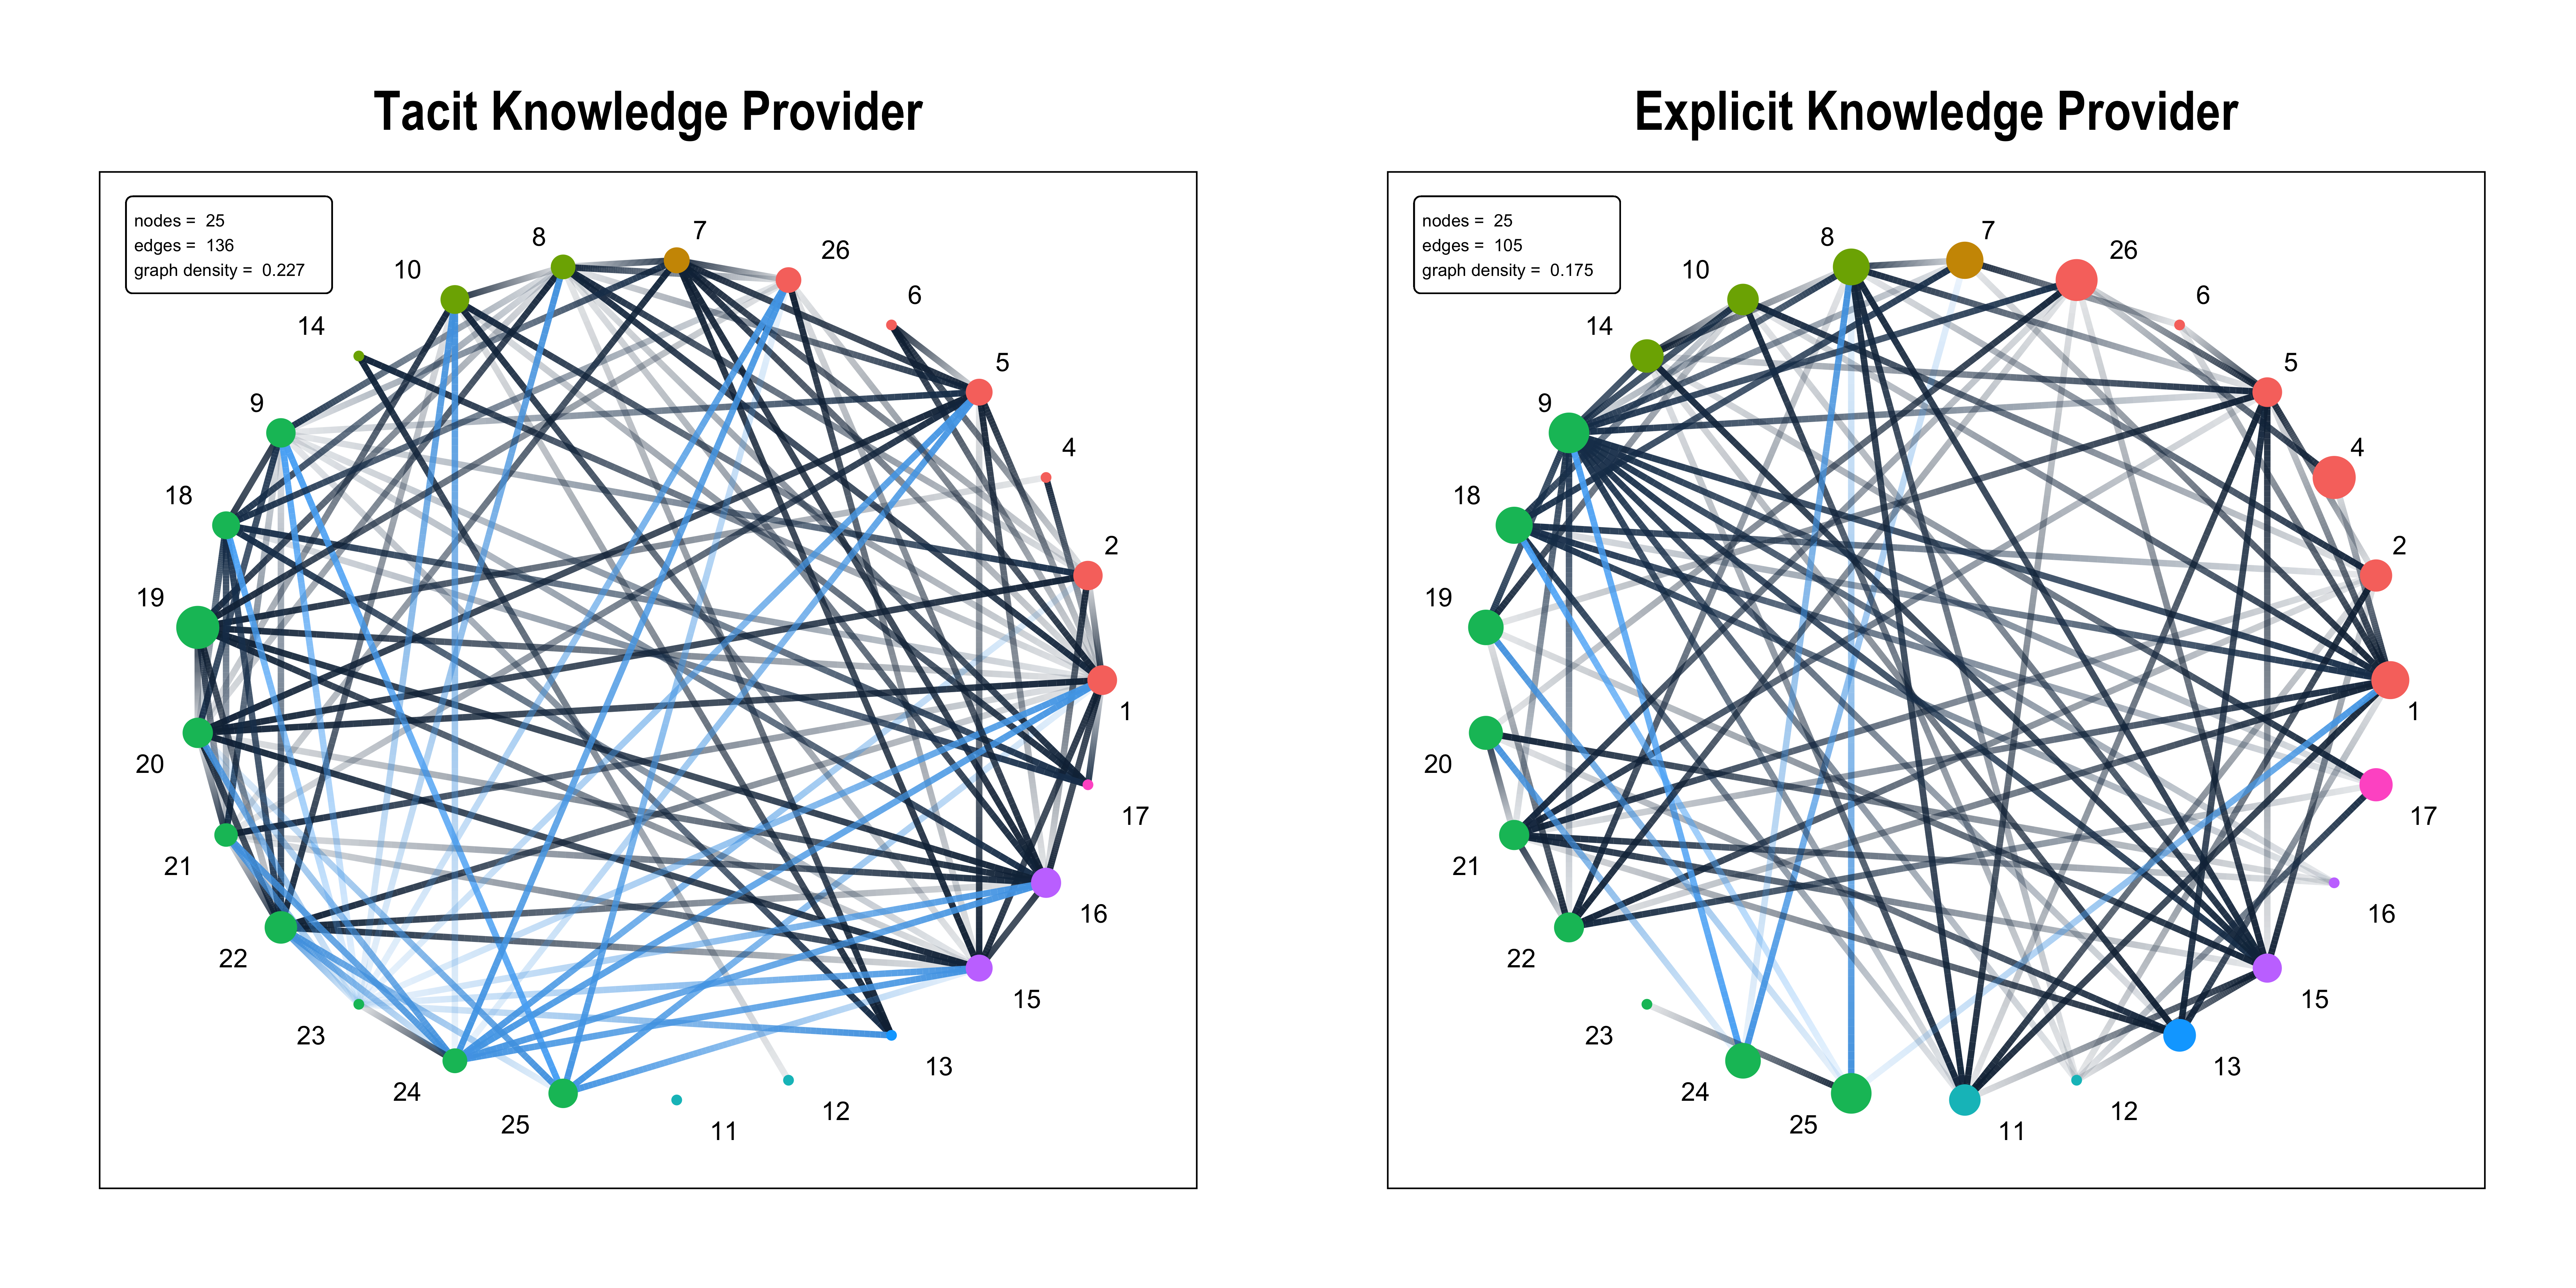
\includegraphics[width=1\linewidth]{Images/networks_case_2.png}
\caption[Knowledge networks for Case 2]{Knowledge networks for Case 2 (see text for an explanation of the different graphical representations).}
\label{fig:network_case_2} 
\end{sidewaysfigure}

\begin{sidewaysfigure}[hbt!]
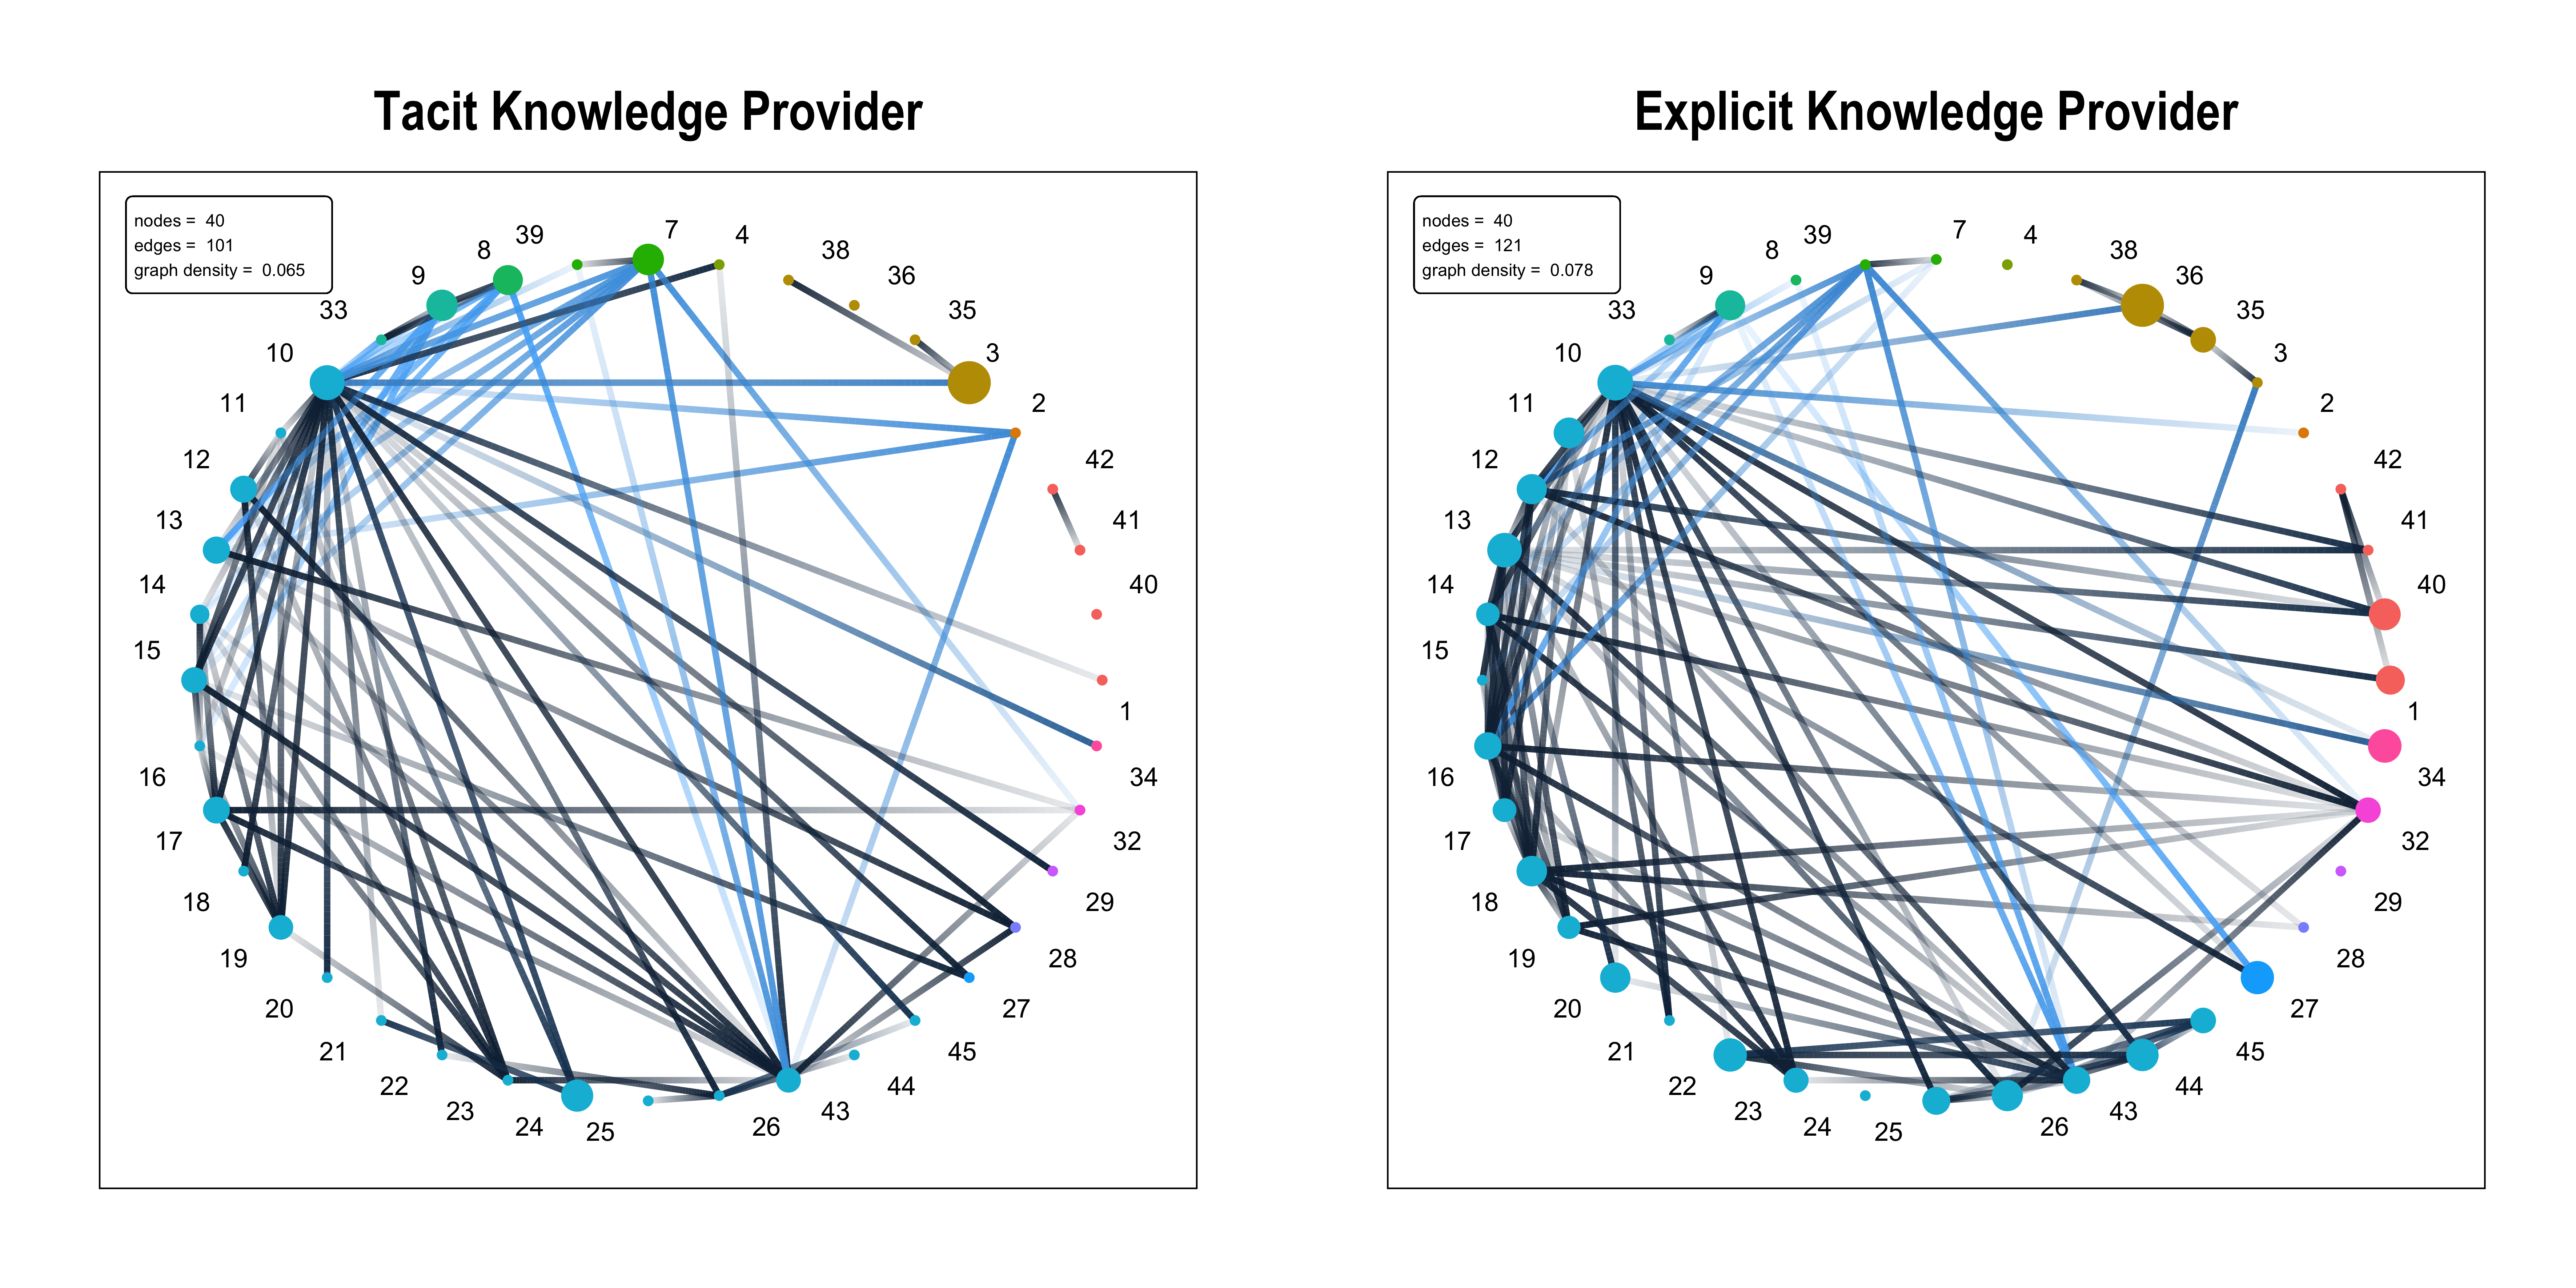
\includegraphics[width=1\linewidth]{Images/networks_case_3.png}
\caption[Knowledge networks for Case 3]{Knowledge networks for Case 3 (see text for an explanation of the different graphical representations).}. 
\label{fig:network_case_3} 
\end{sidewaysfigure}

\subsection{Broker roles}

Brokers are well placed to facilitate the flow of knowledge across organisational boundaries. By examining broker roles, one can assess knowledge diffusion in open innovation partnerships. Figure \ref{fig:gf_brokerage} presents a breakdown of \citeauthor{gould1989structures}'s \citeyearpar{gould1989structures} broker roles by knowledge type in each case (refer to Table \ref{tab:ergm_params} for an explanation of these roles).  \medskip

The mix of broker roles reveals something about knowledge sharing behaviour in each case. Looking at Case 1, the liaison broker role is dominant in the explicit knowledge provider network, indicating that participants are happy to pass on explicit knowledge from one partner to another partner. Some participants operate in a representative broker role, suggesting they are open to sharing their organisation's explicit knowledge with third-parties. The representative broker role is dominant in the tacit knowledge provider network, indicating that participants are open to sharing their organisational know-how and expertise with third-parties. As for Case 2, the liaison role dominates both the explicit and tacit knowledge provider networks. Participants in Case 2 appear willing to pass on all types of knowledge from one partner to another partner, a good sign of collaboration. The internal coordinator role dominates the explicit knowledge provider network in Case 3. Given that almost half the participants in Case 3 work for the same organisation, this is not surprising. The tacit knowledge provider network does not have a dominant broker role. Very few participants operate as itinerant brokers in any of the cases. Note that Figure \ref{fig:gf_brokerage} presents raw broker counts. The statistical significance of the different broker roles receives more attention in Chapter \ref{chp:ergm_result}. \medskip

\begin{figure}[hbt!]
\centering
\includegraphics[width = \linewidth]{Images/gf_brokerage.png}
\caption[Breakdown of broker roles]{Breakdown of \citet{gould1989structures} broker roles. Note $w_I$ = internal coordinator role, $b_O$ = liaison role, $b_{OI}$ = gatekeeper role, $b_{IO}$ = representative role, and $w_O$ = itinerant broker role.}
\label{fig:gf_brokerage}
\end{figure}

\section{Chapter summary}

Case 1 is an example of incremental inbound open innovation. Most of the knowledge exchanged in Case 1 is explicit. However, Case 1 was at an early stage when surveyed. Relationships vital for tacit knowledge exchange were still developing. One can categorise Case 2 as an example of coupled open innovation. Realising a farm system based on voluntary cow traffic is a radical innovation. Tacit knowledge features prominently in Case 2, even though many participants have to collaborate over great distances. This case was in its final stages and participants knew each other reasonably well, which may explain the relatively dense tacit knowledge provider network. Case 3 is an example of outbound open innovation. Using a combination of miniaturised electronic tags and cloud-based data analytics to coordinate honeybee research globally is considered radical innovation. As with Case 2, participants in Case 3 have to collaborate across vast distances. \medskip

The cases are very different in terms of open innovation archetype, the stage at which they are, demographic makeup, and brokerage patterns. One must be careful not to over-generalise the findings from each case. How the unique characteristics of each case shape tacit knowledge sharing will become more apparent in the following chapters. The next chapter (Chapter \ref{chp:ergm_result}) presents the results from the exponential graph modelling. It drills much deeper into the data presented in this chapter. The modelling results will highlight the statistical significance of exogenous factors influencing tacit knowledge sharing in the three open innovation partnerships. 

\chapter{Modelling results} \label{chp:ergm_result}
\section{Introduction}

This chapter introduces the three open innovation cases recruited for this study. We begin with an overview of each case before comparing these in terms of the number of participants, their demographic and psychological attributes, spatial proximity to one another, knowledge sharing ties, and broker roles. All three cases are quite different, and by the end of this chapter, the reader ought to have a good understanding of each. Without this understanding, it will be harder for the reader to make sense of the results from the exponential random graph modelling and analysis of semi-structured interviews presented in Chapters 6 and 7, respectively. \medskip

\begin{sidewaystable}[p]
\centering
\resizebox{0.9\textwidth}{!}{%	
\begin{threeparttable}
\footnotesize
\setlength{\tabcolsep}{6pt}
\renewcommand{\arraystretch}{1}
\caption[Distinguishing  features of the three open innovation cases]{Distinguishing features of the three open innovation cases.}
\label{tab:cases}
\begin{tabular}{@{}cllccccc@{}}
\toprule
Case & \multicolumn{1}{c}{Description} & \multicolumn{1}{c}{Challenge} & \makecell[tc]{Type of \\Open \\Innovation} & Stage & \makecell[tc]{Partner \\organisations} & \makecell[tc]{Identified \\participants} & 
\makecell[tc]{Actual \\participants}\\ \midrule
1 & Cold-chain innovation & \makecell[tl]{Extend shelf-life of green \\leaf vegetables} & Inbound & Early & 7 & 18 & 18\\
2 & Farm system innovation & \makecell[tl]{Implement a robotic \\dairy based on voluntary \\cow traffic} & Coupled & Closing & 8 & 25 & 25 \\
3 & \makecell[tl]{Global honeybee \\research partnership} & \makecell[tl]{Develop a cloud-based data \\analysis system to track \\honeybee movements in and \\out of hives} & Outbound & Very early & 15 & 45 & 40 \\ \bottomrule
\end{tabular}%
\end{threeparttable}
%
}
\end{sidewaystable}

\section{Case overviews}

The distinguishing features of each case are listed in Table \ref{tab:cases}. We are dealing with a small number of individual participants in each case. Two of the cases were at an early stage of execution, while the third was in its closing stage at the time of data collection. Note that partner names have been altered in the case overviews to protect their identity and the geographic markets in which they operate. 

\begin{sidewaysfigure}
\centering
\includegraphics[width = \textwidth]{Images/innovation_types.png}
\caption{Different types of innovation. After \citet{keeley2013ten}.}
\label{fig:innov_type}
\end{sidewaysfigure}

\subsection{Case 1: Cold-chain innovation}

Case 1 revolves around a family-owned business that grows and supplies a range of green leafy vegetable products to caterers, restaurants, local greengrocers, and supermarket chains. Products are supplied either in bulk or in pre-packaged bags sold by the carton. Pre-packaged bags are supplied either as their own branded product or as a supermarket private-label product. The business operates in a region that enjoys a temperate climate, enabling them to grow a greater variety of green leafy vegetables all year round. The business competes with a handful of other firms for supply contracts with national supermarket chains. It views itself as a progressive enterprise that combines innovation, expertise, and a good work ethic, to provide the highest quality fresh produce to its customers. \medskip

\subsubsection{Innovation challenge}

Green leafy vegetable products have a shelf-life of eight days post-production. To maximise product shelf-life, Turner Farms has to deliver products by refrigerated trucks to customers in different parts of the country within two to three days of harvesting. Maintaining uniform air temperatures between 1\si{\degree}C and 4\si{\degree}C in tightly-packed trucks is challenging. Refrigerated air tends to flows around the outside of a load, not through the load, resulting in an uneven temperature distribution that can lead to spoilage. Supermarkets do random checks to check for potential spoilage. Checks involve pushing a temperature probe into a pre-packaged bag or carton. The entire consignment gets rejected if the temperature exceeds a certain threshold. Rejections currently cost the family-owned business between \$100,000 and \$200,000 a year. The business has initiated a program to improve on-farm product handling and packaging practices to reduce spoilage and improve the shelf-life of their products. The general manager responsible for product processing and delivery is driving the cold chain initiative. His goal is to ensure the family-owned business is at the forefront of best-practice. \medskip

The business has excellent working relations with its freight forwarders, all of whom are keen to help it improve on-farm product handling and packaging practices. The freight forwarders do not want to suffer penalties for rejected consignments. It is not always clear if rejections are a result of poor on-farm practices or because of poor temperature control during transit. Working together and sharing practical knowledge is in everybody's best interest. The family-owned business is using advanced wireless micro-sensor technology supplied by a foreign-based firm to gain insight into air temperature variation inside loaded trucks. The foreign-based firm specialises in monitoring the condition of perishable goods through the supply chain. They develop, manufacture, and sell miniaturised wireless sensor devices that can monitor the condition inside individual food packages. Each device can record time and temperature continuously for up to 30 days. Data can be retrieved from each device using wireless data readers up to 100m away, uploaded to a central database, and queried in a variety of ways. The foreign-based firm is helping the family-owned business develop an independent monitoring system to identify problem shipments before they reach their destination. \medskip

The family-owned business has also enlisted the local university to model temperature distributions inside refrigerated trucks using the data provided by the wireless sensor devices. The university recently established a research group to investigate how sensor technology and data analytics can be combined to solve practical problems in perishable goods supply chains. The family-owned business hopes the modelling done by this new research group will lead to better load configurations and packaging material to improve product performance. \medskip

The cold chain initiative is an example of inbound open innovation. Because the aim is to improve on-farm product handling and packaging practices to extend product shelf-life, this case may be considered an example of process and product performance innovation (Figure \ref{fig:innov_type}). 

\subsubsection{Progress to date}

Case 1 was still at an early stage at the time of data collection. Some temperature data had already been collected using the wireless micro-sensor technology provided by the foreign-based firm. Preliminary modelling of air temperature distributions had been completed. A web-based data viewer had been implemented, allowing the family-owned business to monitor product temperature in different parts of the refrigerated truck compartment during transit. \medskip

\subsection{Case 2: Farm system innovation}

Solo Enterprises is a multinational firm specialising in state-of-the-art dairy technology. They have developed the autonomous milk harvester in partnership with Organa Research. The autonomous milk harvester can handle herd sizes of 300 to 800 cows and automates most milking tasks. Apart from creating the potential for significant productivity gains, the autonomous milk harvester does away with the need to have a twice-a-day milking routine, allowing greater flexibility in how a dairy farm operates. Solo Enterprises is piloting its autonomous milk harvester in three countries to see how it performs under different conditions. 

\subsubsection{Innovation challenge}

One pilot is operating on a farm owned by Luke Skywalker. The autonomous milk harvester is suited to either batch milking, voluntary milking, or a combination of both. Batch milking involves bringing the cows in groups to the dairy throughout the day. During milking, the operator can leave the dairy and do other tasks. With voluntary milking, cows walk to the dairy on their own, so there is a steady flow of cows moving through the dairy throughout the day and night. Solo Enterprises, together with its local agent, Chewbacca Dairy Services, and diary researchers from  Organa Research, Jedi Institute, and Obi-Wan Research Centre is helping Luke Skywalker set up a farm system that can handle voluntary milking involving 600 cows. Luke Skywalker hopes this will deliver a more profitable and socially acceptable method of dairy farming.  \medskip

The farm has separate grazing areas with automatic gates that control the movement of cows. Each grazing area opens at a different time over a 24-hour cycle. Cows must pass through drafting gates at the milking area to reach the next fresh pasture break. Adapting the autonomous milk harvester to handle large herds is not without challenges. Optimising the movement of cows through the gates requires a combination of good stockmanship, effective pasture management, and intelligent farm design. Too much pasture encourages cows to linger in the grazing area, resulting in a drop in milking frequency and milk production. On the other hand, too little pasture not only affects cow condition but also leads to an increase in milking frequency, resulting in congestion at the dairy. All this impacts negatively on the operational efficiency of the autonomous milk harvester and ultimately on milk production. 

This project is about intelligent farm design that can accommodate cows' preferred behaviours rather than forcing them into anything. Understanding the complex interplay between cow behaviour, pasture management, feeding regimes, and robot technology has required significant sharing of know-how and expertise. The project is an excellent example of coupled open innovation with Solo Enterprises, Organi Research, and Luke Skywalker working closely together to revolutionise dairy farming (through process, product performance and product system innovation - Figure \ref{fig:innov_type}).  

\subsubsection{Progress to date}

The farm system innovation project was wrapping up at the time of data collection. After five years of ongoing refinement, the innovative farm system that allowed voluntary milking was able to handle a herd of 600 dairy cows. However, the economic benefits of such a system had yet to be assessed. 

\subsection{Case 3: Global honeybee research partnership}

For reasons not fully understood, honeybee colonies around the world are collapsing at an alarming rate. Unchecked, this may lead to food shortages as many crops rely on honeybees for pollination. Research into colony collapse disorder has tended to be piecemeal without a great deal of urgency. Despite the fragmented nature of research into colony collapse disorder, most researchers agree that a key research objective is to gain a deeper understanding of environmental factors that influence honeybee activity. 

\subsubsection{Innovation challenge}

Matrix Laboratories is a multidisciplinary government research agency. They recently developed a novel approach for tracking honeybee movements. Miniaturised electronic tags are attached to honeybees. Sensors register when bees leave and return to the hive. This information is uploaded to a central data repository in near real-time. By massively scaling data collection efforts worldwide, it should be possible to isolate interesting patterns of honeybee movement using sophisticated computer algorithms developed for big data analysis. Finding correlations between patterns of honeybee movement with other environmental information (e.g. local climate variables, traces of pesticides, the co-occurrence of bee predators, or presence of parasites) may shed new light on what is driving colony collapse disorder. However, this does require worldwide coordination of honeybee research. \medskip 

Matrix Laboratories has invited technology providers and honeybee researchers from across the world to work together in a global partnership for coordinated honeybee research. Various technology providers and research institutions across the world have agreed to work together to help coordinate data collection efforts. Matrix Laboratories has been supplying sensor kits to bee researchers to enable them to collect and communicate data to the central data repository. Many bee researchers consider the use of nanosensor technology and big data analysis to be quite revolutionary.
 \medskip

Because Matrix Laboratories is providing its know-how and technology to third-parties, this case is an example of outbound open innovation that is trying to deliver network, structure, process, and service innovations (Figure \ref{fig:innov_type}). It does have the potential to become an example of coupled open innovation should third-parties eventually contribute to the big data analysis. What sets this case apart from the other two cases is the lack of a strong commercial focus. 

\subsubsection{Progress to date}

The global partnership for coordinated honeybee research was in its infancy at the time of data collection. Recruitment of new partners was still ongoing. Existing partners were continuing with their bee research independently of others. Knowledge sharing was limited to issues surrounding the deployment and operation of the miniaturised electronic tag technology. How best to exploit the data collected from across the world was yet to be resolved.  

\section{Case comparison}

\subsection{Participation rates}

A breakdown of the number of partners, number of individual participants, survey response rates, and the number of people interviewed in each case is presented in Table \ref{tab:participation}. Cases 1 and 2 achieved a 100\% survey response rate. Case 3 achieved a 89\% response rate. Of the five participants in Case 3 who declined to participate, two refused outright while the remaining three did not respond at all. The refusals highlighted emerging tensions within the partnership and meant that only 13 of the 15 identified partners were studied. Equipment failure resulted in one interview in Case 3 not being recorded for qualitative analysis. Another interview in Case 3 was cancelled because of foreign language difficulties. Nonetheless, with such high participation rates, one can interpret results with confidence. \medskip

\begin{table}[p]
\centering
\resizebox{\textwidth}{!}{%	
\begin{threeparttable}
\footnotesize
\setlength{\tabcolsep}{6pt}
\renewcommand{\arraystretch}{1}
\caption[Participation rates in each case]{Participation rates in each case.}
\label{tab:participation}
\begin{tabular}{@{}ccccccc@{}}
\toprule
Case & \makecell[tc]{Partner \\organisations} & \makecell[tc]{Individual \\participants} & \makecell[tc]{Survey \\responses} & \makecell[tc]{Response \\rate} & \makecell[tc]{Completed \\interviews} & \makecell[tc]{Interview \\coverage} \\ \midrule
1 & 7 & 18 & 18 & 100\% & 6 & 33\% \\
2 & 8 & 25 & 25 & 100\% & 8 & 32\% \\
3 & 15 & 45 & 40 & 89\% & 8 & 22.5\% \\ \bottomrule
\end{tabular}%
\end{threeparttable}
%
}
\end{table}

\subsection{Demographics}

Figure \ref{fig:demographics} presents key demographic features of each case. It shows how the age, work experience, and job tenure and educational backgrounds of participants vary in each case. The mean age of participants is quite similar across all three cases (the average age ranges between 44 and 45 years). In terms of work experience, Case 1 has the lowest average at 9.2 years, compared to an average of 14.9 years and 13.9 years for Cases 2 and 3, respectively. Case 2 has the highest average job tenure (13.4 years) versus an average of 8.4 years and 9.1 years for Cases 1 and 3, respectively. Though participants in Case 1 are slightly older, they have less experience than the participants in the other two cases. Interestingly, Case 2 has younger but more experienced participants compared to Cases 1 and 3. All the cases have participants with education levels ranging from high school (secondary) level to doctoral level. The educational background of participants in Case 1 is quite diverse, including management and commerce, engineering and related studies, mixed field programmes, agriculture and environmental studies, natural and physical sciences, and education. People with educational backgrounds in agriculture, environmental and related studies dominate Case 2. Case 3 stands out as having the most educated participants (of the 40 participants who responded to the survey, 29 have doctorates). Agricultural, environmental and related studies, and natural and physical sciences are the dominant educational fields in Case 3. \medskip

\begin{figure}
\centering
\begin{subfigure}[b]{0.7\textwidth}
\includegraphics[width=1\linewidth]{Images/age_demographics.png}
\caption{Age, work experience, and tenure.}
%\label{fig:age} 
\end{subfigure}

\begin{subfigure}[b]{0.7\textwidth}
\includegraphics[width=1\linewidth]{Images/ed_level.png}
\caption{Education level}
%\label{fig:ed_level}
\end{subfigure}

\begin{subfigure}[b]{0.7\textwidth}
\includegraphics[width=1\linewidth]{Images/ed_field.png}
\caption{Education field.}
%\label{fig:ed_field}
\end{subfigure}

\caption[Demographic information for each case]{Demographic information for the three open innovation cases.}
\label{fig:demographics}
\end{figure}


\subsection{Psychological attributes}

Figure \ref{fig:psycho} shows the range of different psychological attributes in each case (three of the \enquote{Big Five} personality traits, work motivation, job-related and creative self-efficacy, and identification with workgroup/employer/open innovation partnership). 


\begin{landscape}
\begin{figure*}
\centering
\begin{subfigure}[b]{0.7\textwidth}
\centering
\includegraphics[width=\textwidth]{Images/personality_case.png}
\caption[]%
{{\small Personality traits.}}    
\label{fig:personality}
\end{subfigure}
\hfill
\begin{subfigure}[b]{0.7\textwidth}  
\centering 
\includegraphics[width=\textwidth]{Images/work_motivation_case.png}
\caption[]%
{{\small Work motivation.}}    
\label{fig:motivation}
\end{subfigure}
\vskip\baselineskip
\begin{subfigure}[b]{0.7\textwidth}   
\centering 
\includegraphics[width=\textwidth]{Images/efficacy_case.png}
\caption[]%
{{\small Self-efficacy.}}    
\label{fig:efficacy}
\end{subfigure}
\hfill
\begin{subfigure}[b]{0.7\textwidth}   
\centering 
\includegraphics[width=\textwidth]{Images/identification_case.png}
\caption[]%
{{\small Social identity.}}    
\label{fig:identification}
\end{subfigure}
\caption[Psychological attributes of case participants]
{\small {Psychological attributes of case participants.}} 
\label{fig:psycho}
\end{figure*}
\end{landscape}

\subsection{Geographic proximity}

The geographic spread of participants has implications for tacit knowledge sharing, which generally happens through face-to-face interactions. Participants who are not nearby have fewer opportunities to exchange tacit knowledge with one another. All three cases involve participants based in other countries. Figure \ref{fig:spherical} depicts matrices that show the spherical distance between participants in each case (based on reported workplace postcodes). Case 1 has participants local to each other, in another part of Australia, and one based on another continent. Participants in Case 2 are more spread out. While some participants are local, others are located much further afield, either in another part of the country or another country or continent altogether. Participants in Case 3 are also spread out, with some located on separate continents.  \medskip

\begin{figure}[h!]
\centering
\includegraphics[width = 0.5\linewidth]{Images/proximity.pdf}
\caption[Geographical separation between participants]{Geographical separation between participants.}
\label{fig:spherical}
\end{figure}

\subsection{Network diagrams}

Figures \ref{fig:network_case_1} to \ref{fig:network_case_3} depict the tacit and explicit knowledge provision ties between participants within each case. Nodes are coloured by partner affiliation and sized according to their Everett-Valente brokerage score, where larger nodes have greater access to diverse knowledge. The direction of knowledge flow is indicated by edge shading (flows from light to dark). Edge colours reflect the geographical separation between nodes (lighter colours indicate greater separation). \medskip

Each case has a few highly central actors, some of whom are particularly dominant. The graph densities indicate that the bulk of the knowledge provided in Case 1 is explicit. There is more of an even balance in Case 2, where tacit knowledge provision edges out explicit knowledge provision. Though Case 3 is also more balanced, the density of the explicit knowledge network is slightly higher than that for the tacit knowledge provision network. The graph densities appear to reflect the maturity of each open innovation partnership - the more mature cases tend to have higher graph densities. Edge colours indicate the distance between connected nodes. Lighter colours mean greater separation between nodes. What is notable is the geographic separation between nodes exchanging tacit knowledge. It indicates some participants make a considerable effort to meet face-to-face despite working far apart. \medskip

\begin{sidewaysfigure}
\includegraphics[width=1\linewidth]{Images/networks_case_1.png}
\caption[Knowledge networks for Case 1]{Knowledge networks for Case 1 (see text for an explanation of the different graphical representations).}
\label{fig:network_case_1} 
\end{sidewaysfigure}

\begin{sidewaysfigure}
\includegraphics[width=1\linewidth]{Images/networks_case_2.png}
\caption[Knowledge networks for Case 2]{Knowledge networks for Case 2 (see text for an explanation of the different graphical representations).}
\label{fig:network_case_2} 
\end{sidewaysfigure}

\begin{sidewaysfigure}
\includegraphics[width=1\linewidth]{Images/networks_case_3.png}
\caption[Knowledge networks for Case 3]{Knowledge networks for Case 3 (see text for an explanation of the different graphical representations).}. 
\label{fig:network_case_3} 
\end{sidewaysfigure}

\subsection{Broker roles}

Brokers are well placed to control the flow of knowledge across organisational boundaries. By examining broker roles, one can assess knowledge diffusion in open innovation partnerships. Figure \ref{fig:gf_brokerage} presents a breakdown of \citet{gould1989structures} broker roles by knowledge type in each case (refer to Table \ref{tab:ergm_params} for an explanation of these roles).  \medskip

The mix of broker roles reveals something about knowledge sharing behaviour in each case. Looking at Case 1, the liaison broker role is dominant in the explicit knowledge provider network, indicating participants are happy to pass on explicit knowledge to other partner organisations. Some participants operate in a representative broker role, suggesting they are open to sharing their organisation's explicit knowledge with third-parties. The representative broker role is dominant in the tacit knowledge provider network, indicating that participants are open to sharing their organisational know-how and expertise with third-parties. As to Case 2, the liaison role dominates both the explicit and tacit knowledge provider networks. Participants in Case 2 appear willing to pass on all types of knowledge to third-parties, a good sign of collaboration. The internal coordinator role dominates the explicit knowledge provider network in Case 3. Given that almost half the participants in Case 3 work for the same organisation, this is not surprising. The tacit knowledge provider network does not have a dominant broker role. Very few participants operate as itinerant brokers in any of the cases. \medskip

\begin{figure}
\centering
\includegraphics[width = \linewidth]{Images/gf_brokerage.png}
\caption[Breakdown of broker roles]{Breakdown of \citet{gould1989structures} broker roles. Note $w_I$ = internal coordinator role, $b_O$ = liaison role, $b_{OI}$ = gatekeeper role, $b_{IO}$ = representative role, and $w_O$ = itinerant broker role.}
\label{fig:gf_brokerage}
\end{figure}

\section{Summary}

Each case is quite different. Case 1 is an example of inbound incremental open innovation. Most of the knowledge exchanged in Case 1 is explicit. One can categorise Case 2 is an example of coupled open innovation. Realising a farm system based on voluntary cow traffic is a radical innovation. Case 2 is heavily dependent on tacit knowledge. Many of the participants collaborate over great distances. Case 3 is an example of outbound open innovation. Using a combination of miniaturised electronic tags and big data analytics to coordinate honeybee research on a global basis may be considered radical innovation. As with Case 2, participants in Case 3 have to collaborate across vast distances. \medskip

The three cases were at a different stage of execution at the time of data collection. Cases 1 and 2 were at an early stage, while Case 2 was in its final stage. The average age of participants is quite similar across all three cases. All three cases have participants from diverse educational backgrounds. Case 3 stands out as having the most educated participants. The liaison broker role dominates Cases 1 and 2, a sign of good inter-organisational collaboration. The coordinator broker role dominates Case 3, which is not surprising, given almost half the participants belong to the same organisation. \medskip

The next chapter presents the results from the exponential graph modelling. These should shed light on the psycho-social factors underpinning tacit knowledge sharing in the three open innovation partnerships. 
%
\chapter{Qualitative results} \label{chp:qual_analysis}
\section{Introduction}

Chapter 5 described each of the three cases and contrasted these in terms of their maturity, type of open innovation, demographics, and knowledge provider ties. It revealed the three cases are quite different in terms of the type of open innovation being carried out, how far each had travelled on their open innovation journey, the geographic spread of participants, and the nature of tacit and explicit knowledge exchanges. \medskip

This chapter presents the results of the exponential random graph modelling. The models aim to show which network configurations explain the global structure of observed networks. Recall that network configurations represent underlying social processes or mechanisms. The propositions presented in Chapters 2 and 3 refer to specific social processes or mechanisms pertinent to tacit knowledge sharing in open innovation. Two sets of modelling were done. One set tested propositions about the role of motivation, trust, and power in tacit and explicit knowledge exchanges, while the other set examined the significance of different broker roles in each case. Readers need to be reminded that the online survey asked respondents to name others who provided them with useful and relevant knowledge. As explained in section on data pre-processing in Chapter 4 (Section 4.5.2.5), ties were reversed to depict named knowledge providers as senders of knowledge. \medskip

From a critical realist perspective, the exponential random graph modelling addresses the observed or experienced reality i.e. knowledge sharing events in each case. \medskip

\begin{sidewaystable}[p]
\centering
\resizebox{0.9\textwidth}{!}{%	
\begin{threeparttable}
\footnotesize
\setlength{\tabcolsep}{6pt}
\renewcommand{\arraystretch}{1}
\caption[Parameter estimates for the first set of ERGMs]{ERGM parameter estimates for models exploring motivation, trust and power in tacit and explicit knowledge provider networks. Refer to Table \ref{tab:ergm_params} for an explanation of network parameters.}
\label{tab:ergm_1}
\begin{tabular}{@{}lrrcrrcrr@{}}
\toprule
& \multicolumn{2}{c}{Case 1} &  & \multicolumn{2}{c}{Case 2} &  & \multicolumn{2}{c}{Case 3} \\ \cmidrule(lr){2-3} \cmidrule(lr){5-6} \cmidrule(l){8-9} \multicolumn{1}{c}{} & \multicolumn{1}{c}{Tacit} & \multicolumn{1}{c}{Explicit} & \multicolumn{1}{c}{} & \multicolumn{1}{c}{Tacit} & \multicolumn{1}{c}	{Explicit} & \multicolumn{1}{c}{} & \multicolumn{1}{c}{Tacit} & \multicolumn{1}{c}{Explicit} \\
\cmidrule(lr){2-3} \cmidrule(lr){5-6} \cmidrule(l){8-9} 
\textbf{Purely structural effects (endogenous)} & \multicolumn{1}{l}{} & \multicolumn{1}{l}{} &  & \multicolumn{1}{l}{} & \multicolumn{1}{l}{} &  & \multicolumn{1}{l}{} & \multicolumn{1}{l}{} \\
Arc (edge) & -16.13 (4.39)* & 9.41 (7.03)\phantom{*} &  & -4.59 (1.4)* & -3.73 (1.94)\phantom{*} &  & -7.33 (1.47)* & -2.41 (1.21)\phantom{*} \\
Reciprocity (mutuality) & -1.76 (1.29)\phantom{*} & -2.04 (1.19)\phantom{*} &  & -0.3 (0.65)\phantom{*} & -0.16 (0.93)\phantom{*} &  & -0.45 (0.62)\phantom{*} & -0.75 (0.46)\phantom{*} \\
TwoPath (simple connectivity) & -2.63 (1.60)\phantom{*} & -0.25 (0.24)\phantom{*} &  & -0.01 (0.03)\phantom{*} & 0.08 (0.07)\phantom{*} &  & -0.24 (0.13)\phantom{*} & -0.26 (0.13)* \\
AinS (popularity spread) & -0.87 (0.73)\phantom{*} & 1.82 (0.65)* &  & 0.02 (0.42)\phantom{*} & 0.67 (0.38)\phantom{*} &  & 0.57 (0.34)\phantom{*} & 0.45 (0.29)\phantom{*} \\
AoutS (activity spread) & 0.21 (0.57)\phantom{*} & -5.96 (2.79)* &  & 0.71 (0.40)\phantom{*} & -0.74 (0.80)\phantom{*} &  & 0.89 (0.37)* & 0.36 (0.31)\phantom{*} \\
AT-T (path closure) & 1.93 (0.73)* & 0.50 (0.37)\phantom{*} &  & 0.73 (0.23)* & 0.14 (0.20)\phantom{*} &  & 0.49 (0.26)\phantom{*} & 0.49 (0.25)\phantom{*} \\
A2P-T (multiple connectivity) & 2.58 (1.61)\phantom{*} & 0.37 (0.28)\phantom{*} &  & -0.22 (0.06)* & -0.06 (0.1)\phantom{*} &  & 0.35 (0.13)* & 0.36 (0.14)* \\ \\
\textbf{Actor-relation effects (exogenous)} & \multicolumn{1}{l}{} & \multicolumn{1}{l}{} &  & \multicolumn{1}{l}{} & \multicolumn{1}{l}{} &  & \multicolumn{1}{l}{} & \multicolumn{1}{l}{} \\
Age (difference) & 0.03 (0.04)\phantom{*} & -0.01 (0.02)\phantom{*} &  & 0.00 (0.01)\phantom{*} & 0.00 (0.01)\phantom{*} &  & -0.01 (0.02)\phantom{*} & -0.04 (0.01)* \\
Education level (difference) & -0.34 (0.23)\phantom{*} & 0.18 (0.13)\phantom{*} &  & 0.08 (0.07)\phantom{*} & -0.07 (0.08)\phantom{*} &  & -0.12 (0.11)\phantom{*} & -0.12 (0.11)\phantom{*} \\
Work experience (sender) & 0.00 (0.05)\phantom{*} & -0.12 (0.08)\phantom{*} &  & 0.02 (0.01)* & 0.02 (0.02)\phantom{*} &  & -0.02 (0.02)\phantom{*} & -0.05 (0.02)* \\
Job tenure (sender) & 0.06 (0.06)\phantom{*} & 0.18 (0.09)* &  & 0.00 (0.01)\phantom{*} & -0.01 (0.02)\phantom{*} &  & 0.04 (0.02)\phantom{*} & 0.07 (0.03)* \\
Openness (sender) & 1.19 (2.29)\phantom{*} & -3.92 (3.85)\phantom{*} &  & -0.35 (0.47)\phantom{*} & 0.13 (0.92)\phantom{*} &  & 0.06 (0.63)\phantom{*} & -0.46 (0.68)\phantom{*} \\
Openness (receiver) & 6.19 (2.58)* & -0.66 (1.29)\phantom{*} &  & -0.18 (0.67)\phantom{*} & 0.2 (0.69)\phantom{*} &  & -1.08 (0.64)\phantom{*} & 0.61 (0.59)\phantom{*} \\
Controlled motivation (sender) & -0.89 (1.88)\phantom{*} & -12.22 (4.84)* &  & 0.56 (0.68)\phantom{*} & 2.16 (1.34)\phantom{*} &  & 2.84 (1.01)* & 1.25 (0.85)\phantom{*} \\
Controlled motivation (receiver) & -2.44 (2.90)\phantom{*} & 1.61 (1.42)\phantom{*} &  & -1.53 (0.84)\phantom{*} & -1.23 (0.93)\phantom{*} &  & -2.69 (0.94)* & 0.67 (0.71)\phantom{*} \\
Autonomous motivation (sender) & 1.80 (2.12)\phantom{*} & -0.67 (2.32)\phantom{*} &  & 0.21 (0.52)\phantom{*} & -1.93 (1.11)\phantom{*} &  & -0.24 (0.88)\phantom{*} & -1.08 (0.7)\phantom{*} \\
Autonomous motivation (receiver) & 9.35 (3.03)* & -1.22 (1.12)\phantom{*} &  & 1.53 (0.75)* & 1.61 (0.90)\phantom{*} &  & 3.62 (1.12)* & -0.15 (0.69)\phantom{*} \\
Identification with group (sender) & 0.13 (1.13)\phantom{*} & -0.36 (1.54)\phantom{*} &  & 0.00 (0.33)\phantom{*} & 1.77 (0.79)* &  & -1.19 (0.48)* & -0.1 (0.42)\phantom{*} \\
Identification with group (receiver) & 2.05 (1.62)\phantom{*} & -0.91 (0.77)\phantom{*} &  & 0.02 (0.47)\phantom{*} & -0.08 (0.38)\phantom{*} &  & -0.08 (0.42)\phantom{*} & -0.11 (0.39)\phantom{*} \\
Employer (match) & 0.07 (0.86)\phantom{*} & 2.36 (0.89)* &  & 0.77 (0.32)* & 0.64 (1.05)\phantom{*} &  & 0.61 (0.35)\phantom{*} & 0.46 (0.31)\phantom{*} \\
Employer (mismatch reciprocity) & -8.74 (22.83)\phantom{*} & 3.79 (1.32)* &  & 0.71 (0.68)\phantom{*} & 0.48 (0.26)\phantom{*} &  & 1.92 (0.83)* & -0.42 (1.21)\phantom{*} \\ \\
\textbf{Dyadic covariate effects (exogenous)} & \multicolumn{1}{l}{} & \multicolumn{1}{l}{} &  & \multicolumn{1}{l}{} & \multicolumn{1}{l}{} &  & \multicolumn{1}{l}{} & \multicolumn{1}{l}{} \\
Cognition-based tust & 2.75 (0.79)* & 2.53 (0.56)* &  & 0.78 (0.21)* & 0.96 (0.40)* &  & 1.47 (0.33)* & 0.34 (0.28)\phantom{*} \\
Reporting hierarchy & 0.47 (0.81)\phantom{*} & 0.31 (0.68)\phantom{*} &  & -1.02 (0.48)* & -0.01 (0.05)\phantom{*} &  & 0.62 (0.50)\phantom{*} & 0.84 (0.4)* \\
Geographic proximity & -0.26 (0.13)* & 0.08 (0.09)\phantom{*} &  & 0.00 (0.04)\phantom{*} & 0.00 (0.00)\phantom{*} &  & -0.08 (0.05)\phantom{*} & -0.22 (0.05)* \\ \bottomrule
\end{tabular}

\begin{tablenotes}
\footnotesize
\item[a] Estimates are significant (*) when the absolute value of the parameter estimate is more than twice the magnitude of the estimated standard error.
\item[b] Goodness of fit scores for non-explicitly modelled statistics were less than 2 in all models, a, and less than 0.1 for all explicitly modelled effects, indicating the models provide adequate fit to most aspects of the social structure.

\end{tablenotes}

\end{threeparttable}
%
}
\end{sidewaystable}

\section{Models exploring motivation, trust and power}

The first set of models examined how autonomous motivation, cognition-based trust, and reporting hierarchy shape tacit and explicit knowledge sharing ties in each case. \medskip

Parameters used in the first set of models included controlled and autonomous sender/receiver effects (to determine to what extent the two types of motivation predict knowledge sharing) and cognition-based trust and reporting hierarchy dyadic covariate effects (to check to what extent knowledge sharing ties align with cognition-based trust ties and reporting hierarchy ties). Other parameters controlled for network structure (reciprocity, simple and multiple connectivity, popularity and activity spread, and transitive closure), homophily (age and education level difference, employer match), personality (openness to experience sender/receiver), social identity (identification with group sender/receiver), reciprocal exchanges across organisational boundaries (employer mismatch reciprocity), and geographic proximity (log of kilometre distance). Results for each case are presented side-by-side in Table \ref{tab:ergm_1}. \medskip

Apart from modelling each case separately, each case's networks were combined and modelled as one big network. Combining the tacit and explicit knowledge provider networks allows one to see which model parameters are significant across all three cases. Table \ref{tab:ergm_2} presents the results of the combined network analysis.

\subsection{Case 1: Cold-chain innovation}

Looking at the results for Case 1, parameter estimates for the tacit knowledge provider network show significant and positive effects for path closure (AT-T = 1.93), openness to experience (receiver = 6.19), autonomous motivation (receiver = 9.35), and cognition-based trust (dyadic covariate = 2.75). These effects suggest participants prefer to share their tacit knowledge with others they have strong ties with. The significant and positive receiver effects reflect a strong learning orientation, i.e. participants who are open to experience and autonomously motivated are more likely to seek out tacit knowledge. The significant and negative effect observed for geographic proximity (dyadic covariate = -0.26) indicates that tacit knowledge is more likely to be exchanged with others who are nearby.  \medskip

As to the explicit knowledge provider network, parameter estimates show significant and positive effects for popularity spread (AinS = 1.82), job tenure (sender = 0.18), employer (match = 2.36 and mismatch reciprocity = 3.79), and cognition-based trust (dyadic covariate = 2.53). In other words, participants are likely to direct explicit knowledge to a few actors they trust. Explicit knowledge tends to be provided by participants who have been in the job for some time. There is also a tendency to exchange explicit knowledge with others from the same organisation. That there is also a significant two-way exchange of explicit knowledge across organisational boundaries is a sign of good collaboration. The significant and negative effect for activity spread suggests explicit knowledge is being provided evenly by many participants, not by a few active individuals. Moreover, participants are not feeling pressured to provide explicit knowledge, judging from the significant and negative controlled motivation (sender) effect. Formal structure is not significant in the explicit knowledge provider network. This suggests that structure is not interfering with or inhibiting agency that much ( \medskip 

\subsection{Case 2: Farm system innovation}

Modelling of the tacit knowledge provider network yields significant and positive effects for path closure (AT-T = 0.73), work experience (sender = 0.02), autonomous motivation (receiver = 1.53), and cognition-based trust (dyadic covariate = 0.78). The effects for path closure and cognition-based trust indicate participants prefer to share their tacit knowledge with others they trust. Recipients of tacit knowledge also tend to be autonomously motivated. This suggests they have a strong learning orientation. There are significant and negative effects for both multiple connectivity (A2P = -0.22) and reporting hierarchy (dyadic covariate = -1.02). The combination of a significant and positive effect for path closure and a significant and negative effect for multiple connectivity is a sign of good collaboration. Participants are sufficiently well-connected that brokerage is no longer required. The significant and negative effect for reporting hierarchy indicates that tacit knowledge sharing happens mostly through informal structures. Geographic proximity is not a significant factor in the tacit knowledge provider network. \medskip

With respect to the explicit knowledge provider network, the estimates only show significant and positive effects for identification with group (sender = 1.77) and cognition-based trust (dyadic covariate = 0.96). Explicit knowledge is more likely to be provided to trusted others and those they identify strongly with. 

\subsection{Case 3: Global partnership for honeybee research}

Estimates for the tacit knowledge provider network show significant and positive effects for activity spread (AoutS = 0.89), multiple connectivity (A2P = 0.35), controlled motivation (sender = 2.81), autonomous motivation (receiver = 3.62), employer (mismatch reciprocity = 1.92), and cognition-based trust (dyadic covariate = 1.47). The significant and positive effect for activity spread suggests tacit knowledge is being provided by a relatively small number of participants. Participants are also more likely to share their tacit knowledge with others they trust. The significant and positive effect for multiple connectivity is an indicator of substantial brokerage. As with the other cases, recipients of tacit knowledge tend to be autonomously motivated. The significant and positive effect for controlled motivation (sender) suggests, contrary to expectations, that many participants feel obliged to share their tacit knowledge. There is a significant two-way exchange of tacit knowledge across organisational boundaries, judging by the significant and positive effect for employer (mismatch reciprocity). \medskip

In terms of the explicit knowledge provider network, the estimates show significant and positive effects for multiple connectivity (A2P = 0.36), job tenure (sender = 0.07), and reporting hierarchy (dyadic covariate = 0.84). In other words, much of the explicit knowledge flowing through the network is coming from participants who have been in their job for some time. Explicit knowledge also tends to flow up the reporting hierarchy. The estimates show significant and negative effects for simple connectivity (TwoPath = -0.26), age (difference = -0.04), work experience (sender = -0.05), and geographic proximity (dyadic covariate = -0.22). These indicate that received explicit knowledge is not passed on, age homophily is not a factor in explicit knowledge exchanges, and that more experienced participants are less likely to share explicit knowledge with others. Explicit knowledge is also more likely to be exchanged with nearby participants. 

\subsection{Analysis of the combined networks}

\begin{table}[]
\centering
\resizebox{0.9\textwidth}{!}{	
\begin{threeparttable}
\footnotesize
\setlength{\tabcolsep}{6pt}
\renewcommand{\arraystretch}{1}
\caption{ERGM parameter estimates for the combined tacit and explicit knowledge provider networks.}
\label{tab:ergm_2}
\begin{tabular}{@{}lrlr@{}}
\toprule
 & \multicolumn{3}{c}{Cases 1 + 2 + 3} \\ \cmidrule(l){2-4} 
 & \multicolumn{1}{c}{Tacit} &  & \multicolumn{1}{c}{Explicit} \\ \cmidrule(lr){2-2} \cmidrule(l){4-4} 
\textbf{Purely structural effects (endogenous)} &  &  &  \\
Arc (edge) & -4.66 (0.71)* &  & -2.95 (0.83)* \\
Reciprocity (mutuality) & -0.37 (0.39)\phantom{*} &  & -0.51 (0.37)\phantom{*} \\
TwoPath (simple connectivity) & -0.05 (0.04)\phantom{*} &  & -0.09 (0.06)\phantom{*} \\
AinS (popularity spread) & 0.01 (0.18)\phantom{*} &  & 0.63 (0.19)* \\
AoutS (activity spread) & 0.63 (0.18)* &  & 0.05 (0.21)\phantom{*} \\
AT-T (path closure) & 0.84 (0.17)* &  & 0.56 (0.13)* \\
A2P-T (multiple connectivity) & 0.01 (0.05)\phantom{*} &  & 0.09 (0.08)\phantom{*} \\
&  &  &  \\
\textbf{Actor-relation effects (exogenous)} &  &  &  \\
Age (difference) & -0.01 (0.01)\phantom{*} &  & -0.01 (0.01)\phantom{*} \\
Education level (difference) & 0.08 (0.04)* &  & 0.03 (0.04)\phantom{*} \\
Work experience (sender) & 0.00 (0.01)\phantom{*} &  & -0.01 (0.01)\phantom{*} \\
Job tenure (sender) & 0.00 (0.01)\phantom{*} &  & 0.01 (0.01)\phantom{*} \\
Openness (sender) & -0.53 (0.34)\phantom{*} &  & -0.33 (0.41)\phantom{*} \\
Openness (receiver) & -0.31 (0.39)\phantom{*} &  & 0.20 (0.32)\phantom{*} \\
Controlled motivation (sender) & 0.55 (0.57)\phantom{*} &  & 0.56 (0.62)\phantom{*} \\
Controlled motivation (receiver) & -0.76 (0.64)\phantom{*} &  & -0.32 (0.48)\phantom{*} \\
Autonomous motivation (sender) & -0.62 (0.39)\phantom{*} &  & -1.29 (0.44)* \\
Autonomous motivation (receiver) & 1.71 (0.54)* &  & 0.12 (0.39)\phantom{*} \\
Identification with group (sender) & 0.08 (0.23)\phantom{*} &  & 0.14 (0.27)\phantom{*} \\
Identification with group (receiver) & -0.32 (0.25)\phantom{*} &  & 0.25 (0.22)\phantom{*} \\
Employer (match) & 0.47 (0.16)* &  & 0.49 (0.16)* \\
Employer (mismatch reciprocity) & 0.77 (0.46)\phantom{*} &  & 1.07 (0.45)* \\
 &  &  &  \\
\textbf{Dyadic covariate effects (exogenous)} &  &  &  \\
Cognition-based trust & 1.26 (0.16)* &  & 0.89 (0.16)* \\
Reporting hierarchy & 0.30 (0.24)\phantom{*} &  & 0.82 (0.22)* \\
Geographic proximity & 0.00 (0.02)\phantom{*} &  & -0.07 (0.02)* \\ \bottomrule
\end{tabular}
\begin{tablenotes}
\footnotesize
\item[a] Estimates are significant (*) when the absolute value of the parameter estimate is more than twice the magnitude of the estimated standard error.
\item[b] Goodness of fit scores were less than 2 for more than 97.85\% of the non-explicitly modelled statistics, indicating the models provide adequate fit to most aspects of the knowledge exchange structure.
%\item[c] Given each partnership had a different number of participants (18, 25, and 40 participants in Cases 1, 2, and 3 respectively) and each partnership's maturity when surveyed, one must not read too much into these estimates.
\end{tablenotes}
\end{threeparttable}
}
\end{table}

Parameter estimates for the combined tacit knowledge network show that across all three cases, there is a significant and positive effect for activity spread and path closure (0.63 and 0.84, respectively). One can infer from this that knowledgeable people are happy to share their know-how with others in their group. The significant and positive effect for age difference (0.08) indicates that people are more likely to share knowledge with others of a similar age (across all three cases, there is age homophily effect). As with each case, the significant and positive autonomous motivation (receiver) effect (1.71) suggests most tacit knowledge recipients are autonomously motivated. The significant and positive employer (match) effect (0.47) indicates that people are inclined to share their tacit knowledge with others employed in the same organisation. People also tend to share their know-how with others they deem trustworthy (significant and positive cognition-based trust dyadic covariate effect = 1.26). \medskip

In contrast, parameter estimates for the combined explicit knowledge provider network show a significant and positive effect for popularity spread (0.63), indicating that across the three cases, explicit knowledge tends to flow to more central actors. Moreover, the significant and positive dyadic covariate effect for reporting hierarchy (0.82) suggests these central actors occupy senior positions. The significant and positive path closure effect (0.56) indicates that explicit knowledge sharing mostly occurs within well-connected groups. Interestingly, the significant and negative autonomous motivation (sender) effect (-1.29) suggests that across the three cases, autonomously motivated people are less likely to share explicit knowledge. Explicit knowledge tends to be shared with others employed by the same organisation (significant and positive employer (match) effect = 0.49). However, the significant and positive employer (mismatch reciprocity) effect (1.07) indicates that explicit knowledge exchanges among open innovation partners tends to be reciprocal. People are also inclined to share explicit knowledge with people they trust (significant and positive dyadic cognition-based trust covariate effect = 0.89) and who are nearby (significant and negative geographic proximity dyadic covariate effect = -0.07).  

\section{Models examining broker roles}

The second set of models examining the significance of broker roles in each case used fewer parameters than the first set, just path closure and the five broker roles. Path closure was included to highlight the tension between network closure and brokerage. Results from the second set of modelling are presented in Table \ref{tab:ergm_3}. These must be considered in light of the broker role counts presented in Figure \ref{fig:gf_brokerage} and the results from the first set of models. Despite including only the five broker roles plus an edge and/or path closure effect, the models assessing the significance of broker roles are able explain most of the observed network configurations. It appears one can characterise open innovation partnerships in terms of path closure and broker roles alone. \medskip 

\begin{sidewaystable}[p]
\centering
\resizebox{0.9\textwidth}{!}{%	
\begin{threeparttable}
\footnotesize
\setlength{\tabcolsep}{6pt}
\renewcommand{\arraystretch}{1}
\caption[Parameter estimates for the second set of ERGMs]{ERGM parameter estimates for models assessing broker roles. Refer to Table \ref{tab:ergm_params} for an explanation of network parameters.}
\label{tab:ergm_3}
\begin{tabular}{@{}lrrlrrlrr@{}}
\toprule
\multicolumn{1}{c}{} & \multicolumn{2}{c}{Case 1} & \multicolumn{1}{c}{} & \multicolumn{2}{c}{Case 2} & \multicolumn{1}{c}{} & \multicolumn{2}{c}{Case 3} \\ \cmidrule(lr){2-3} \cmidrule(lr){5-6} \cmidrule(l){8-9} 
\multicolumn{1}{c}{} & \multicolumn{1}{c}{Tacit} & \multicolumn{1}{c}{Explicit} & \multicolumn{1}{c}{} & \multicolumn{1}{c}{Tacit} & \multicolumn{1}{c}{Explicit} & \multicolumn{1}{c}{} & \multicolumn{1}{c}{Tacit} & \multicolumn{1}{c}{Explicit} \\ \cmidrule(lr){2-3} \cmidrule(lr){5-6} \cmidrule(l){8-9} 
\textbf{Purely structural effects (endogenous)} & \multicolumn{1}{l}{} & \multicolumn{1}{l}{} &  & \multicolumn{1}{l}{} & \multicolumn{1}{l}{} &  & \multicolumn{1}{l}{} & \multicolumn{1}{l}{} \\
Arc (edge) & -2.56 (0.23)* & -2.47 (0.29)* &  & -2.52 (0.31)* & -2.34 (0.31)* &  & -3.13 (0.12)* & -3.09 (0.15)* \\
ATA-T (path closure) & 0.73 (0.34)* & 0.85 (0.14)* &  & 1.06 (0.12)* & 0.57 (0.12)* &  & \makecell[c]{---} & 0.81 (0.11)* \\ \\
\textbf{Actor-brokerage effects (exogenous)} & \multicolumn{1}{l}{} & \multicolumn{1}{l}{} &  & \multicolumn{1}{l}{} & \multicolumn{1}{l}{} &  & \multicolumn{1}{l}{} & \multicolumn{1}{l}{} \\
$w_O$ (liaison) & -0.39 (0.19)\phantom{*} & -0.11 (0.08)\phantom{*} &  & -0.22 (0.06)* & -0.04 (0.06)\phantom{*} &  & 0.04 (0.06)\phantom{*} & -0.2 (0.09)* \\
$w_I$ (coordinator) & -0.15 (0.46)\phantom{*} & -0.1 (0.29)\phantom{*} &  & -0.05 (0.19)\phantom{*} & -0.09 (0.19)\phantom{*} &  & 0.04 (0.06)\phantom{*} & -0.01 (0.04)\phantom{*} \\
$b_{OI}$ (gatekeeper) & -0.55 (0.99)\phantom{*} & 0.07 (0.12)\phantom{*} &  & -0.17 (0.11)* & -0.02 (0.11)\phantom{*} &  & 0.32 (0.05)* & 0.06 (0.05)\phantom{*} \\
$b_{IO}$ (representative) & 0.42 (0.56)* & -0.07 (0.14)\phantom{*} &  & -0.19 (0.1)* & 0.01 (0.1)\phantom{*} &  & 0.33 (0.03)* & 0.05 (0.06)\phantom{*} \\
$b_O$ (itinerant broker) & -0.63 (0.46)\phantom{*} & -0.62 (0.34)\phantom{*} &  & -0.15 (0.11)\phantom{*} & -0.07 (0.11)\phantom{*} &  & -1.54 (0.48)* & -0.42 (0.23)\phantom{*} \\
 \bottomrule
\end{tabular}
\begin{tablenotes}
\footnotesize
\item[a] Estimates are significant (*) when the absolute value of the parameter estimate is more than twice the magnitude of the estimated standard error.
\item[b] Path closure was not modelled in the Case 3 tacit knowledge network. Inclusion of this parameter resulted in a degenerate model. Despite this, the goodness-of-fit in this particular model was excellent (t-ratios $<2$ for 97\% of the non-explicitly modelled statistics).
\item[c] Goodness of fit scores were less than 2 for 98.3\% of the non-explicitly modelled statistics, and less than 0.1 for all explicitly modelled parameters, indicating the models provide adequate fit to most aspects of the social structure.

\end{tablenotes}

\end{threeparttable}
%
}
\end{sidewaystable}

\subsection{Case 1: Cold-chain innovation}

The parameter estimates presented in Table \ref{tab:ergm_1} indicate brokerage does not feature strongly in either the tacit and explicit knowledge networks.  Looking at the broker role counts presented in Figure \ref{fig:gf_brokerage}, the representative role dominates the broker role counts for the tacit knowledge network. The parameter estimates presented in Table \ref{tab:ergm_2} confirm that the representative role is significant in the tacit knowledge network ($b_{IO}$ = 0.42). It appears participants are happy to pass on internal tacit knowledge to others working for different organisations. Though the liaison role dominates the broker role counts in the explicit knowledge network, the parameter estimates indicate this role is not significant. \medskip

Whereas the models exploring autonomous motivation, cognition-based trust, and reporting hierarchy show a significant and positive effect for path closure in the tacit knowledge network only, the more simple models examining broker roles show a significant and positive effect for path closure in both the tacit and explicit knowledge networks (AT-T = 0.73 and 0.85, respectively). Path closure was included to highlight the tension between network closure and brokerage. The significant and positive effect for path closure indicates network closure is more dominant than brokerage in both networks. 

\subsection{Case 2: Farm system innovation}

The parameter estimates presented in Table \ref{tab:ergm_1} show that there is significantly less brokerage and significantly more clustering in the tacit knowledge network. This combination is a sign of excellent collaboration. Given this case was winding up at the time of data collection, this is not surprising. Brokers are unlikely to feature in well-established partnerships. Although the liaison role domineers broker role counts in both the tacit and explicit knowledge networks, the modelling of broker roles shows this role is under-represented in the tacit knowledge network ($w_0$ = -0.22) and not significant in the explicit knowledge network. The modelling also reveals that the gatekeeper and representative roles are significantly under-represented in the tacit knowledge network ($b_{IO}$ = -0.17, $b_{OI}$ = -0.19). 

\subsection{Case 3: Global partnership for honeybee research}

The parameter estimates presented in Table \ref{tab:ergm_1} suggest brokerage is significant in both the tacit and explicit knowledge networks. Considering this case was at a very early stage at the time of data collection, this is not unexpected. The absence of significant and positive effects for path closure in both networks suggests brokerage is the dominant network process. However, the parameter estimates presented in Table \ref{tab:ergm_2} are contradictory. These show a significant and positive effect for path closure in the explicit knowledge network (AT-T = 0.81). Unfortunately, path closure could not be modelled in the tacit knowledge network. Inclusion of this parameter resulted in a degenerate model. The significant and positive effect for path closure in the explicit knowledge network does indicate path closure is the more dominant network process. \medskip 

Looking at the broker role counts presented in Figure \ref{fig:gf_brokerage}, the itinerant broker role hardly features in either the tacit or explicit knowledge networks. Other roles are evenly spread in the tacit knowledge network, while the coordinator role dominates the explicit knowledge network, the modelling of broker roles show a significant and positive effect for both the gatekeeper and representative role in the tacit knowledge network ($b_{IO}$ = 0.32, $b_{OI}$ = 0.33). The modelling confirms that the itinerant broker role is significantly under-represented in the tacit knowledge network ($b_O$ = -1.54). Apart from the significant and negative effect for the liaison role ($w_O$ = -0.2), there are no significant broker role effects in the explicit knowledge network. \medskip  

\section{Summary}

Though each open innovation partnership is different, some network effects are common to two or more cases. Concerning the first set of models, the tacit knowledge provider networks exhibit significant path closure in Case 1 and Case 2. Path closure indicates that know-how features strongly in group practice. Tacit knowledge brokerage is significantly under-represented in Case 2 and significantly over-represented in Case 3 (. The opposite effects reflect the maturity of each partnership. Case 2 is quite mature with well-established groups, unlike Case 3, which is still in its formative stages. \medskip

All three cases have a significant autonomous motivation receiver effect in their tacit knowledge provider networks, indicating that learning features prominently in all three cases. Cognition-based trust is a significant dyadic covariate in all but one of the knowledge provider networks (it was not significant in the Case 3 explicit knowledge provider network). Participants are more likely to share their know-how and know-what with others they trust. \medskip

Concerning the second set of models assessing broker roles, path closure was significant in all but one of the knowledge provider networks (it was not possible to model path closure in the Case 3 tacit knowledge provider network). All three tacit knowledge provider networks had significant representative broker role effects. More specifically, Case 1 and 3 had a positive effect, unlike Case 2, which had a negative effect. Significant negative and positive gatekeeper role effects feature in Case 2 and Case 3 tacit knowledge provider networks, respectively. The representative and gatekeeper broker roles appear to be less critical in established tacit knowledge networks. \medskip

From a critical realist perspective, the exponential random graph modelling accounts for the observed or experienced reality. The next chapter presents the results from the qualitative analysis, which should shed light on contextual factors that influenced knowledge sharing (what happens in actual practice).
%
\chapter{Cross-case analysis} \label{chp:cross_case}
\section{Introduction}

From a critical realist perspective, the ERGM results presented in Chapter 6 reflect observed reality. We are dealing with knowledge of what is perceived to be happening \citep{bhaskar2013realist}. Whereas ERGMs are very useful for measuring patterns of perceived social interaction, they do not capture the broader context in which this social interaction occurs. This chapter presents the results from the qualitative analysis of the semi-structured interviews and should shed light on the unmeasured or actual reality, i.e. knowledge of what happens. \medskip

This study employs the agency model proposed by \citet{loyal2001agency} to evaluate the propositions developed in Chapters 2 and 3. The propositions suggest that individuals exchange tacit knowledge to satisfy an innate need for self-determination and because of social expectations or norms. Tempering the decision to share or seek tacit knowledge are external factors such as the presence of boundaries (e.g. organisational, disciplinary, or cultural boundaries), rules of engagement (e.g. contractual arrangements, appropriability regimes), trust (i.e. interpersonal and inter-organisational trust), and power relations (e.g.power-over versus power-to). Skilled brokerage is seen to play a crucial role in helping individuals overcome boundaries, build trust, and manage power relations. The qualitative analysis aims to test the validity of the propositions. \medskip

Unlike the ERGM analysis, which employs deductive logic to test propositions about social interactions, the qualitative analysis uses first- and second-cycle coding to unpack the psychosocial mechanisms that shape tacit knowledge sharing relations in open innovation partnerships. First-cycle coding employs inductive logic to expand a set of provisional codes derived from the propositions into sub-codes that unpack how different social mechanisms operate in practice (see Table \ref{tab:provcode} for the list of the provisional codes). Second-cycle coding uses the logic of retroduction to group the sub-codes into categorical codes. The categorical codes refer to the main components of the \citet{loyal2001agency}'s agency model. \medskip

To get a better sense of the participants interviewed and the weight of their opinions or views, this chapter begins by introducing the interviewees in terms of their role in their respective open innovation partnership, self-reported personal information, and position in their respective knowledge-sharing networks. The chapter then presents the results of the first- and second-cycle coding for each case before concluding with a summary of the leading social mechanisms at play in each partnership.

\begin{table}[]
\centering
\caption[Provisional codes]{Provisional codes derived from theoretical propositions.}
\label{tab:provcode}
%\renewcommand{\arraystretch}{1.2}
\resizebox{0.9\textwidth}{!}{%	
\begin{tabular}{l p{0.4\linewidth}}
\toprule
\multicolumn{1}{c}{Proposition} & \multicolumn{1}{c}{Provisional codes} \\ \midrule
\multirow{2}{*}{\begin{minipage}{0.7\linewidth}
\begin{enumerate}
    \item[1a] Open innovation requires practitioners to connect across real and perceived boundaries to apply their know-how in novel ways.
\end{enumerate}
\end{minipage}} & Real and perceived boundaries \\
 & Doing something novel \\ \\ 
\multirow{2}{*}{\begin{minipage}{0.7\linewidth}
\begin{enumerate}
    \item[1b] Reducing cognitive distance between open innovation partners requires significant social interaction to support learning and the application of knowledge in practice.
\end{enumerate}
\end{minipage}} & Learning \\ 
& Applying knowledge in practice \\ \\ \\
\multirow{2}{*}{\begin{minipage}{0.7\linewidth}
\begin{enumerate}
    \item[2a] Successful open innovation requires a combination of skilled brokerage and network closure.
\end{enumerate}
\end{minipage}} & Brokering exchanges \\
& Collaborating \\ \\ 
\multirow{2}{*}{\begin{minipage}{0.7\linewidth}
\begin{enumerate}
    \item[3a] Formal structures inhibit tacit knowledge exchange in open innovation partnerships.
\end{enumerate}
\end{minipage}} & Rules of engagement \\
& Power structures \\ \\
\multirow{3}{*}{\begin{minipage}{0.7\linewidth}
\begin{enumerate}
    \item[3b] Individual needs dispositions and internalised social norms moderate a person's willingness to seek out or share tacit knowledge.
\end{enumerate}
\end{minipage}} & Satisfying innate needs \\
& Expressing a particular worldview \\
& Identifying with a distinct group \\ \\
\multirow{1}{*}{\begin{minipage}{0.7\linewidth}
\begin{enumerate}
    \item[4a] Reciprocity and closure in tacit knowledge exchange networks indicate high levels of trust in open innovation partnerships.
\end{enumerate}
\end{minipage}} & Trust relations \\ \\  \\
 \multirow{2}{*}{\begin{minipage}{0.7\linewidth}
 \begin{enumerate}
    \item[4b] Who people choose to empower with their know-how depends on how much they trust the receiver to use their know-how in mutually beneficial ways.
\end{enumerate} 
 \end{minipage}}
& Empowering others \\
& Selective revealing \\  \\ \bottomrule
\end{tabular}
}
\end{table}

\section{Participant information}

One aim of the qualitative analysis was to interview a cross-section of participants in terms of their partner affiliation and knowledge network centrality (i.e. central and peripheral actors in the knowledge provider networks). Unfortunately, some targeted participants were either not available or unwilling to be interviewed. Despite not being able to interview all the targeted people, participants who were eventually interviewed revealed much about the social dynamics in each partnership. The interviews covered 33\% of Case 1 participants, 32\% of Case 2 participants, and 17.5\% of Case 3 participants. Most of the participants interviewed reside in Australia. Of the 21 interviews conducted, 13 were face-to-face and the rest done via video-link. Two participants who live abroad were interviewed face-to-face while visiting Australia. \medskip

Table \ref{tab:interviewees} provides a breakdown of the participants interviewed in each case. Interviews ranged from 25 to 106 minutes in duration. Longer interviews tend to bias the qualitative analysis (such interviews are assigned more codes). The longer interviews usually involved participants with higher network centrality. Their privileged network position meant they were well-placed to provide useful information about knowledge exchanges. \medskip

\begin{sidewaystable}[p]
\centering
\caption[Details about each interview]{Details about each interview.}
\label{tab:interviewees}
\resizebox{\textwidth}{!}{%       
\begin{threeparttable}
\begin{tabular}{crrcrc l ccccccccc}
\toprule

& \specialcell[t]{Network\\Id} &
\specialcell[t]{Employer} &
\specialcell[t]{Date of\\interview} &
\specialcell[t]{Duration\\(MM:SS)} &
\specialcell[t]{Interview\\mode} &
\multicolumn{1}{c}{Role} &
\specialcell[t]{Gender} &
\specialcell[t]{Age} &
\specialcell[t]{Education\\level} &
\specialcell[t]{Relevant\\experience\\(years)} &
\specialcell[t]{Job tenure\\(years)} &
\specialcell[t]{Openness} &
\specialcell[t]{Network\\centrality} &
\specialcell[t]{Country} \\ 
\midrule
\multirow{6}{*}{\rotatebox[origin=c]{90}{Case 1} \rotatebox[origin=c]{90}{($n = 18$)}} 
& 1/1 & 1/1 & 18.12.2015 & 79:04 & F2F & General Manager & M & 54 & 6 & 9 & 4 & 0.44 & 31 & AU \\
& 3/1 & 1/1 & 26.04.2016 & 33:34 & F2F & Transport Manager & M & 51 & 2 & 10 & 19 & 0.61 & 18 & AU \\
& 8/1 & 2/1 & 11.03.2016 & 81:01 & F2F & Company Director & M & 62 & 3 & 12 & 12 & 0.78 & 12 & AU \\
& 10/1 & 3/1 & 07.03.2016 & 58:46 & F2F & Director International Sales & M & 44 & 7 & 16 & 9 & 0.72 & 2 & USA \\
& 15/1 & 7/1 & 25.02.2016 & 66:29 & F2F & Research Engineer & M & 51 & 7 & 25 & 1 & 0.72 & 11 & AU \\
& 16/1 & 7/1 & 07.09.2016 & 43:35 & F2F & Research Group Leader & M & 53 & 8 & 16 & 1 & 0.50 & 9 & AU \\ 
\midrule
\multirow{8}{*}{\rotatebox[origin=c]{90}{Case 2} \rotatebox[origin=c]{90}{($n = 25$)}} 
& 1/2 & 1/2 & 01.03.2016 & 59:21 & F2F & Dairy Farmer & M & 28 & 6 & 7 & 7 & 0.44 & 39 & AU \\
& 8/2 & 2/2 & 18.03.2016 & 70:02 & VL & Research Project Leader & F & 41 & 8 & 14 & 10 & 0.50 & 28 & AU \\
& 9/2 & 3/2 & 20.03.2016 & 106:10 & F2F & Farm Systems Manager & M & 46 & 6 & 18 & 8 & 0.78 & 40 & NZ \\
& 10/2 & 4/2 & 18.03.2016 & 48:44 & VL & Technical Specialist & M & 32 & 8 & 10 & 2 & 0.61 & 18 & AU \\
& 11/2 & 5/2 & 04.03.2016 & 66:04 & F2F & Pasture Specialist & M & 58 & 6 & 25 & 8 & 0.78 & 11 & AU \\
& 15/2 & 7/2 & 03.11.2016 & 76:13 & F2F & Company Director & M & 50 & 4 & 25 & 19 & 0.50 & 34 & AU \\
& 18/2 & 3/2 & 16.02.2016 & 69:02 & VL & Executive Oversight & M & 68 & 5 & 35 & 5 & 0.44 & 26 & NZ \\ 
& 23/2 & 3/2 & 11.03.2016 & 24:53 & VL & Technical Specialist & M & 44 & 3 & 25 & 20 & 0.67 & 15 & SE \\ 
\midrule
\multirow{7}{*}{\rotatebox[origin=c]{90}{Case 3} \rotatebox[origin=c]{90}{($n = 40$)}} 
& 9/3 & 9/3 & 14.12.2016 & 61:35 & VL & Research Scientist & M & 50 & 8 & 26 & 26 & 0.61 & 18 & BR \\
& 10/3 & 10/3 & 16.03.2016 & 89:26 & F2F & Research Leader & M & 45 & 8 & 8 & 3 & 0.78 & 70 & AU \\
& 13/3 & 10/3 & 13.05.2016 & 35:42 & F2F & Project Coordinator & F & 41 & 8 & 4 & 4 & 0.72 & 35 & AU \\
& 16/3 & 10/3 & 12.09.2016 & 73:23 & F2F & Technical Specialist & M & 47 & 7 & 16 & 9 & 0.89 & 23 & AU \\ 
& 22/3 & 10/3 & 19.09.2016 & 47:48 & VL & Executive Oversight & M & 61 & 8 & 32 & 32 & 0.53 & 10 & AU \\ 
& 39/3 & 7/3 & 09.09.2016 & 27:14 & VL & Technical Specialist & M & 30 & 7 & 4 & 2 & 0.61 & 10 & MX \\
& 41/3 & 1/3 & 07.10.2016 & 32:36 & VL & Technical Specialist & M & 24 & 6 & 5 & 4 & 0.78 & 3 & NZ \\
\bottomrule
\end{tabular}
\begin{tablenotes}
% \footnotesize
\item[i] $n$ refers to the number of respondents to the online survey.
\item[ii] Education level is based on the Australian Standard Classification for Education, ranging from 2 (secondary education) to 8 (doctoral qualification).
\item[iii] F2F refers to face-to-face interviews, whereas VL refers to \texttt{Skype}\texttrademark\ interviews. 
\item[iv] Network centrality refers to number of incoming and outgoing social ties in the combined (tacit and explicit) knowledge network.
\end{tablenotes}
\end{threeparttable}
}
\end{sidewaystable}


\begin{table}[]
\centering
\caption[Breakdown of sentiment]{Breakdown of sentiment by interviewee. Participants in Case 1 are generally quite positive, unlike the other two cases, where the less positive sentiment is an indicator of some tension in these cases.}
\begin{subtable}{1\textwidth}
\centering
\resizebox{\textwidth}{!}{%   
\begin{tabular}{r *{4}{c}}
\toprule
\multicolumn{1}{c}{}
Network id & Very negative & Moderately negative & Moderately positive & Very positive \\ \midrule
1/1 & \gradientcell{24}{0}{50}{lime}{red}{90} & \gradientcell{26}{0}{50}{lime}{red}{90} & \gradientcell{46}{0}{50}{lime}{red}{90} & \gradientcell{13}{0}{50}{lime}{red}{90} \\
3/1 & \gradientcell{2}{0}{50}{lime}{red}{90} & \gradientcell{4}{0}{50}{lime}{red}{90} & \gradientcell{19}{0}{50}{lime}{red}{90} & \gradientcell{14}{0}{50}{lime}{red}{90} \\
8/1 & \gradientcell{16}{0}{50}{lime}{red}{90} & \gradientcell{23}{0}{50}{lime}{red}{90} & \gradientcell{37}{0}{50}{lime}{red}{90} & \gradientcell{12}{0}{50}{lime}{red}{90} \\
10/1 & \gradientcell{14}{0}{50}{lime}{red}{90} & \gradientcell{13}{0}{50}{lime}{red}{90} & \gradientcell{45}{0}{50}{lime}{red}{90} & \gradientcell{22}{0}{50}{lime}{red}{90} \\
15/1 & \gradientcell{11}{0}{50}{lime}{red}{90} & \gradientcell{18}{0}{50}{lime}{red}{90} & \gradientcell{35}{0}{50}{lime}{red}{90} & \gradientcell{10}{0}{50}{lime}{red}{90} \\
16/1 & \gradientcell{6}{0}{50}{lime}{red}{90} & \gradientcell{8}{0}{50}{lime}{red}{90} & \gradientcell{28}{0}{50}{lime}{red}{90} & \gradientcell{9}{0}{50}{lime}{red}{90} \\ \bottomrule
\end{tabular}
}%
\bigskip
\caption{Case 1}
\label{tab:sentiment_case_1}
\end{subtable}

\bigskip
\begin{subtable}{1\textwidth}
\centering
\resizebox{\textwidth}{!}{%   
\begin{tabular}{r *{4}{c}}
\toprule
\multicolumn{1}{c}{}
Network id & Very negative & Moderately negative & Moderately positive & Very positive \\ \midrule
1/2 & \gradientcell{16}{0}{80}{lime}{red}{90} & \gradientcell{28}{0}{80}{lime}{red}{90} & \gradientcell{27}{0}{80}{lime}{red}{90} & \gradientcell{17}{0}{80}{lime}{red}{90} \\
8/2 & \gradientcell{11}{0}{80}{lime}{red}{90} & \gradientcell{17}{0}{80}{lime}{red}{90} & \gradientcell{33}{0}{80}{lime}{red}{90} & \gradientcell{23}{0}{80}{lime}{red}{90} \\
9/2 & \gradientcell{30}{0}{80}{lime}{red}{90} & \gradientcell{27}{0}{80}{lime}{red}{90} & \gradientcell{72}{0}{80}{lime}{red}{90} & \gradientcell{18}{0}{80}{lime}{red}{90} \\
10/2 & \gradientcell{6}{0}{80}{lime}{red}{90} & \gradientcell{6}{0}{80}{lime}{red}{90} & \gradientcell{42}{0}{80}{lime}{red}{90} & \gradientcell{11}{0}{80}{lime}{red}{90} \\
11/2 & \gradientcell{23}{0}{80}{lime}{red}{90} & \gradientcell{22}{0}{80}{lime}{red}{90} & \gradientcell{44}{0}{80}{lime}{red}{90} & \gradientcell{22}{0}{80}{lime}{red}{90} \\
15/2 & \gradientcell{25}{0}{80}{lime}{red}{90} & \gradientcell{39}{0}{80}{lime}{red}{90} & \gradientcell{41}{0}{80}{lime}{red}{90} & \gradientcell{22}{0}{80}{lime}{red}{90} \\
18/2 & \gradientcell{8}{0}{80}{lime}{red}{90} & \gradientcell{8}{0}{80}{lime}{red}{90} & \gradientcell{42}{0}{80}{lime}{red}{90} & \gradientcell{15}{0}{80}{lime}{red}{90} \\
23/2 & \gradientcell{2}{0}{80}{lime}{red}{90} & \gradientcell{3}{0}{80}{lime}{red}{90} & \gradientcell{10}{0}{80}{lime}{red}{90} & \gradientcell{5}{0}{80}{lime}{red}{90} \\ \bottomrule
\end{tabular}
}%
\bigskip
\caption{Case 2}
\label{tab:sentiment_case_2}
\end{subtable}

\bigskip
\begin{subtable}{1\textwidth}
\centering
\resizebox{\textwidth}{!}{%   
\begin{tabular}{r *{4}{c}}
\toprule
\multicolumn{1}{c}{}
Network id & Very negative & Moderately negative & Moderately positive & Very positive \\ \midrule
9/3 & \gradientcell{2}{0}{70}{lime}{red}{90} & \gradientcell{6}{0}{70}{lime}{red}{90} & \gradientcell{12}{0}{70}{lime}{red}{90} & \gradientcell{5}{0}{70}{lime}{red}{90} \\
10/3 & \gradientcell{15}{0}{70}{lime}{red}{90} & \gradientcell{24}{0}{70}{lime}{red}{90} & \gradientcell{66}{0}{70}{lime}{red}{90} & \gradientcell{28}{0}{70}{lime}{red}{90} \\
13/3 & \gradientcell{7}{0}{70}{lime}{red}{90} & \gradientcell{11}{0}{70}{lime}{red}{90} & \gradientcell{21}{0}{70}{lime}{red}{90} & \gradientcell{5}{0}{70}{lime}{red}{90} \\
16/3 & \gradientcell{14}{0}{70}{lime}{red}{90} & \gradientcell{19}{0}{70}{lime}{red}{90} & \gradientcell{47}{0}{70}{lime}{red}{90} & \gradientcell{22}{0}{70}{lime}{red}{90} \\
22/3 & \gradientcell{13}{0}{70}{lime}{red}{90} & \gradientcell{12}{0}{70}{lime}{red}{90} & \gradientcell{23}{0}{70}{lime}{red}{90} & \gradientcell{15}{0}{70}{lime}{red}{90} \\
39/3 & \gradientcell{1}{0}{70}{lime}{red}{90} & \gradientcell{4}{0}{70}{lime}{red}{90} & \gradientcell{2}{0}{70}{lime}{red}{90} & \gradientcell{2}{0}{70}{lime}{red}{90} \\
41/3 & \gradientcell{5}{0}{70}{lime}{red}{90} & \gradientcell{4}{0}{70}{lime}{red}{90} & \gradientcell{11}{0}{70}{lime}{red}{90} & \gradientcell{7}{0}{70}{lime}{red}{90} \\ \bottomrule
\end{tabular}
}%
\bigskip
\caption{Case 3}
\label{tab:sentiment_case_3}
\end{subtable}
\end{table}

\begin{figure}
\centering
\begin{subfigure}[b]{0.7\textwidth}
\includegraphics[width=1\linewidth]{Images/bigram_c1.pdf}
\caption{Case 1}
\label{fig:bigram_case_1} 
\end{subfigure}
\bigskip
\begin{subfigure}[b]{0.7\textwidth}
\includegraphics[width=1\linewidth]{Images/bigram_c2.pdf}
\caption{Case 2}
\label{fig:bigram_case_2}
\end{subfigure}
\bigskip
\begin{subfigure}[b]{0.7\textwidth}
\includegraphics[width=1\linewidth]{Images/bigram_c3.pdf}
\caption{Case 3}
\label{fig:bigram_case_3}
\end{subfigure}
\caption[Bigram word-clouds from interviews]{Bigram word-clouds highlighting what interviewees from each case mainly spoke about.}
\label{fig:bigrams}
\end{figure}


\section{Case 1}

\subsection{Semi-structured interviews}

Six people were interviewed face-to-face in Case 1 (Table \ref{tab:interviewees}). Due to scheduling conflicts, it took nine months to complete all the interviews. The length of the interviews ranged between 34 and 81 minutes (the average interview duration was 60 minutes). Table \ref{tab:sentiment_case_1} shows the overall sentiment expressed by interviewees from Case 1. Most of them were positive about the open innovation partnership. Figure \ref{fig:bigram_case_1} highlights what the interviewees mainly spoke about. Topics that stand out include \enquote{cold air}, \enquote{cold/supply chain}, \enquote{shelf-life}, and \enquote{freight companies}.

\subsection{Recap of network analysis}

The tacit knowledge provider network is quite sparse, suggesting that tacit knowledge is not important in Case 1. The ERGM results indicate people are more likely to share tacit knowledge with others in their immediate social group. Receivers of tacit knowledge tend to be trusted, open to experience, and autonomously motivated. Geography is a limiting factor for tacit knowledge exchanges. Explicit knowledge mostly flows to a few central actors who are likely to be from the same organisation. Providers of explicit knowledge tend to have been in their jobs for some time. \medskip

The modelling of broker roles shows that the representative broker role dominates tacit knowledge exchanges. Explicit knowledge exchanges are more likely to involve liaison brokers (Table \ref{tab:ergm_3}). Whereas the modelling assesses whether broker roles are under or over-represented for all possible two-path configurations, the raw broker counts presented in Figure \ref{fig:gf_c1} allow one to assess dominant brokers in the network. For example, Participant 1/1 stands out as the dominant broker, acting primarily in a liaison and gatekeeper role in the explicit knowledge network and a lesser extent in a representative and internal coordinator role in the tacit knowledge network. Responses to semi-structured interview questions help us understand how Participant 1/1 influenced knowledge flows in both networks.  

\begin{figure}
\centering
\includegraphics[width = \textwidth]{Images/gf_case1.pdf}
\caption[Breakdown of broker roles by participant in Case 1]{Breakdown of broker roles by participant in Case 1. Note $w_I$ = internal coordinator role, $b_O$ = liaison role, $b_{OI}$ = gatekeeper role, $b_{IO}$ = representative role, and $w_O$ = itinerant broker role. Participant 1/1 stands out as a dominant broker.}
\label{fig:gf_c1}
\end{figure}

\subsection{Coding results}

Table \ref{tab:case_1_codes} lists the most referenced codes in each category for Case 1. Innate needs and subjective norms did not feature strongly in responses to interview questions. Nonetheless, the desire to perform interesting and meaningful work was an important motivator. However, the sharing of know-how appears to be tempered by participants with a narrow outlook, who resist change, or consider themselves intellectually superior to others. Key mechanisms and structures moderating tacit knowledge exchanges include the need to have good relations to facilitate open and honest discussions, swift trust, difficulty accessing knowledgeable people and poor communication. Actions revolved around broadening understanding to improve practices, tapping external expertise, and brokering (or restricting) knowledge exchanges. 

\begin{sidewaystable}
\centering
\caption{Top codes in each category: Case 1.}
\label{tab:case_1_codes}
\begin{tabular}{lllc}
\toprule
Category code & Provisional code & Detailed code & References \\ 
\midrule
Innate needs & Motivational forces & Desire to do meaningful work &   5 \\
Subjective norms & Expressing a particular worldview & Maintaining a narrow perspective &   6 \\ 
Subjective norms & Expressing a particular worldview & Superior attitude &   4 \\ 
Subjective norms & Expressing a particular worldview & Resisting change &   3 \\ 
Mechanisms \& structures & Trust relations & Having good relations &  10 \\ 
Mechanisms \& structures & Trust relations & Having open and honest discussions &  10 \\ 
Mechanisms \& structures & Trust relations & Swift trust &   9 \\ 
Mechanisms \& structures & Boundaries & Engaging with busy people &   9 \\ 
Mechanisms \& structures & Boundaries & Poor communication &   8 \\ 
Action & Applying knowledge in practice & Improving practices &  30 \\ 
Action & Brokering exchanges & Liaison brokerage &  17 \\ 
Action & Learning & Broaden understanding &  16 \\ 
Action & Learning & Tapping external expertise &  15 \\ 
Action & Brokering exchanges & Gate-keeping &  11 \\ 
\bottomrule
\end{tabular}
\end{sidewaystable}

\subsubsection{Innate needs}

Although the social network analysis suggests receivers of tacit knowledge tend to be autonomously motivated people, the need for competence, autonomy, or social connectedness did not feature strongly in the responses to interview questions. Only the university participants stated they were motivated by a desire to do meaningful and exciting work:

\begin{quote}
\small
\enquote{being seen to be involved in [a particular region] with a major producer out there doing things, hopefully producing something that is meaningful.} \\
\rightline{\rm --- Participant 15/1}
\end{quote}

\begin{quote}
\small
\enquote{I think for any researcher, if you think the work that you do will actually be utilised and you can see evidence of it, well that’s a pretty big kick.} \\
\rightline{\rm --- Participant 16/1}
\end{quote}

\subsubsection{Subjective norms}

The interviews reveal doubts about the absorptive capacity of the refrigerated transport companies. A couple of the interviewees did not believe the freight companies would be able to grasp scientific ideas:

\begin{quote}
\small
\enquote{I don't think they ever look at it scientifically, I think they just look at it very broadly, and that's as far as they go.} \\
\rightline{\rm --- Participant 1/1}
\end{quote}

\begin{quote}
\small
\enquote{if you were talking to [the freight company] yeah, you don't want to start talking about thermal masses and all that sort of stuff.} \\
\rightline{\rm --- Participant 15/1}
\end{quote}

Not wanting to explain things in any great detail denied the freight companies the opportunity to learn more about thermodynamics, which is disappointing given the owner of the main freight company had a strong desire to learn about and implement good cold chain practices:

\begin{quote}
\small
\enquote{ I've always been very, very conscious, and maybe fanatical about having facilities that can keep product cold ... so with that you learn about air flow, and cold air and what's best and what’s not best, and you take advice from people who make the fridges, and who make the vans, and who talk about insulation ... for the last 22 or 23 years of my life I've [been a student of] refrigerated transport.} \\
\rightline{\rm --- Participant 8/1}
\end{quote}

\begin{quote}
\small
\enquote{the guy who we spoke to was the owner [of the freight company] - he was really interested. So I think what happened was that there was an interest level that was really driving it more than anything else.} \\
\rightline{\rm --- Participant 16/1}
\end{quote}

The big supermarket customers are quite prescriptive in how they work with their suppliers. The general manager driving the cold chain initiative was afraid that his supermarket customers would not be receptive to any suggested changes to the way orders are handled:

\begin{quote}
\small
\enquote{I go back to my customer and say, \enquote{Hey, I really need you to order your product in a much more... in a much better way} ... if they just say to us, \enquote{No, look, this is how we do things, we’re not going to help you there}, I’m screwed.} \\
\rightline{\rm --- Participant 1/1}
\end{quote}

Supermarkets consider food safety to be much more important than extending the shelf-life of fresh produce. Reducing contamination risk dictates how products are packaged, even if this means fresh produce cannot be adequately chilled:

\begin{quote}
\small
\enquote{[the product] is in a bag that's not conducive to letting the air get into, or the product to remain cold. Then it gets put into a carton. That is a complete box that’s sealed. It used to have holes in it, and then [the one big supermarket customer] says you can't have holes, because people can contaminate it. So if you want my honest answer, right there, right then, you're wasting your time having refrigeration. Because the air's not going to [chill the product], the air's only keeping the carton cold.} \\
\rightline{\rm --- Participant 8/1}
\end{quote}

\subsubsection{Mechanisms & structures}

Being able to have open discussions, accessing busy people, and selective communication are the main social mechanisms affecting knowledge exchanges in Case 1. The social network analysis highlights the importance of cognition-based trust for tacit knowledge sharing. One indicator of trust is the ability to have open and honest discussions. Not only do open and honest discussions help build trust, trust also enables open and honest discussions:

\begin{quote}
\small
\enquote{I think that over time you can build up trust, and then you can share your knowledge and different things like that.} \\
\rightline{\rm --- Participant 3/1}
\end{quote}

\begin{quote}
\small
\enquote{the amount of information shared is less if I do not trust the person and trust, in my opinion, can be built up over time.} \\
\rightline{\rm --- Participant 10/1}
\end{quote}

One of the university researchers made an interesting point about the relationship between explicit and tacit knowledge sharing:

\begin{quote}
\small
\enquote{explicit knowledge sharing comes after you've built the relationships that enable tacit knowledge [exchange].} \\
\rightline{\rm --- Participant 15/1}
\end{quote}

The manager of freight logistics at the green leafy vegetable grower made an interesting point about sharing of tacit knowledge:

\begin{quote}
\small
\enquote{Whereas I might think it's very important for someone to share this knowledge so we can actually look at improving different things, but they may not think it's that important.} \\
\rightline{\rm --- Participant 3/1}
\end{quote}

Participants may withhold tacit knowledge because they do not consider their know-how is worth sharing. They discount the value of their knowledge. According to the owner of the main freight company, trust allows one to engage in difficult conversations that help surface problems and bring these into sharper focus. He believes it is easier to resolve problems this way:   

\begin{quote}
\small
\enquote{We can have those conversations, because you need to, it's healthy to be able to debate the issue ... The fact that we have tension, and that we create tension, is because we trust each other ... because tension is created by a cock up, if you want to put it that way. So what's the best way to fix that problem? Be innovative, or fix it.} \\
\rightline{\rm --- Participant 8/1}
\end{quote}

Swift trust did feature in this open innovation partnership. The general manager driving the cold chain initiative did not know the university researchers well but assumed they were competent and knew what they were doing:

\begin{quote}
\small
\enquote{when [the head of the university team] came along and introduced me to his team, I do form an opinion on who I'm working with by ... you know, and I spend a bit of time talking to them and that sort of stuff. So, but I suppose, too, part of the whole, you know part of this whole collaboration thing with the university is that I suppose you have to trust the people that you’re going to work with ... I'm trusting them that they know what they're doing and why they're doing it, and what they're going to be able to get out of it at the end of it.} \\
\rightline{\rm --- Participant 1/1}
\end{quote}
 
One of the biggest obstacles to knowledge sharing was finding time to engage with busy people. The university researchers initially struggled to gain access to people with relevant know-how in the green leafy vegetable operation:   

\begin{quote}
\small
\enquote{initially, trying to get contact with [the green leafy vegetable grower] was challenging at times, as you'd understand when you're trying to do research with a company because they've got operational imperatives that they need to manage and they have day-to-day crises that they need to manage.} \\
\rightline{\rm --- Participant 16/1}
\end{quote}

However, as relationships developed and research credibility was established, it became easier for the university researchers to connect with personnel at the green leafy vegetable operation:

\begin{quote}
\small
\enquote{what I really noticed was as we started to go through the process and building up credibility, [the green leafy vegetable grower] could see there were potential outcomes here, then they were ringing us more.} \\
\rightline{\rm --- Participant 16/1}
\end{quote}

Interestingly, the general manager felt his organisation suffered from a silo mentality that affected the sharing of knowledge and/or ideas: 

\begin{quote}
\small
\enquote{there’s this silo mentality in the business that we need to break, and I think once you've broken that then you'll... then there will be a lot more idea sharing, and a lot more new things that we want to do and want to try out.} \\
\rightline{\rm --- Participant 1/1}
\end{quote}

The general manager has not been very open himself, being somewhat selective with his communication. His transport manager, for example, expresses some frustration at not being kept in the loop about the results of experimental trials:

\begin{quote}
\small
\enquote{I haven't honestly seen a real lot of the results from the different university trials and things like that. So from my point of view it probably hasn't been as open as what it could be ... I'm not quite sure why the knowledge hasn't been passed down, or whether it's been passed to other people and not to me. I don't know.} \\
\rightline{\rm --- Participant 3/1}
\end{quote}

Given the transport manager is a central actor in both the tacit and explicit knowledge provider networks (Figure \ref{fig:network_case_1}), it does seem odd to leave him out of the communication loop. The experimental trials do relate to the transport manager's area of responsibility. Not keeping him abreast of developments has caused some resentment and may explain why he was not particularly forthcoming in his interview (his interview was the shortest, taking just 34 minutes to complete). \medskip

\subsubsection{Actions}

How people apply knowledge in practice, broker connections, or engage in learning are the actions that stand out in Case 1. The cold-chain initiative is all about prolonging the shelf life of green leafy vegetables through improved cold chain practices:

\begin{quote}
\small
\enquote{it'll allow us to ... work on better methods to transport our product, and get to a point where we know that when we send our product that we've packed it and palletised it, and loaded it into the vans in the best possible manner, which will give us the best possible outcome throughout the journey.} \\
\rightline{\rm --- Participant 1/1}
\end{quote}

The freight company owner was pleased the green leafy vegetable grower was tapping into their refrigerated transport expertise:

\begin{quote}
\small
\enquote{the fact that they’re actually talking to a service provider about what's best practice for them, based on our knowledge.} \\
\rightline{\rm --- Participant 8/1}
\end{quote}

One example of this are the new loading docks. The freight company advised the grower on how best to set up their loading docks: 

\begin{quote}
\small
\enquote{so we go down to their facility, have a look around, there's your floor. There's your slope. This is where you should put your docks. You need 37 metres for a normal truck to be able to back. And then you need to have a little bit more in case the driver who gets the foot, we step it out. These timing docks with the air bags and the ramp is fine. You need it to be 1.2 metres high, because that’s an average height of your van. So you need to dig this out, or put concrete or gravel down. No, no, you need to do concrete, because you've got the trucks that need to be secure. You can't have them sinking, you'll be filling in potholes all the time. You'll need to spend money on concrete. You need to do this, you need to do that. You need to have doors that go up and down. You need to have doors that can open, allow the vans to open. So that when you put your four or five pallets in, you can close the doors and keep the temperature in the van.} \\
\rightline{\rm --- Participant 8/1}
\end{quote}

The general manager facilitated interaction between the university and other parts of his organisation (operating in a liaison broker role):

\begin{quote}
\small
\enquote{And I also put them in touch with people on the processing side and the farm side, so they could, if they wanted to ask any further questions they could. Especially for processing, one of the key things is around product shelf-life, and you know what impacts product shelf-life. So we've got a couple of people here who do data shelf life testing, and they have a fairly strong view on what impacts shelf-life, you know, and after all like our product gets washed and dried, and then put in a bag, so you've got this like micro-environment there, and nobody really knows what happens in there, and I felt that they needed to understand that.} \\
\rightline{\rm --- Participant 1/1}
\end{quote}

He also saw himself as an interpreter, helping the freight companies understand understand the experiments the university researchers were attempting: 

\begin{quote}
\small
\enquote{I believe I'm pretty good at doing is just explaining something that is slightly more complicated in a much simpler fashion, so and relate it to more day to day stuff. So the way I interact with the [university] guys when they're here, and the way I interact with the freight companies, and the people that work there, completely different.} \\
\rightline{\rm --- Participant 1/1}
\end{quote}

However, the general manager was also a gatekeeper, not allowing university researchers to directly engage freight providers. He argued that allowing the university researchers too much independence would be quite disruptive: 

\begin{quote}
\small
\enquote{I said to the [university] that if they need to spend some time with [the freight company] and use some of their equipment, that I'm the person who paves the way for them to go there and do it, rather than them doing it, because I'm the one who sort of spoke to the service providers and we’re all in agreement that there's something in it for all of us. So, but it's really it just needs one person to co-ordinate it, because if I had three or four people ringing up [the freight company] saying \enquote{Oh, we want to do this, we want to do that}”, it would be quite messy.} \\
\rightline{\rm --- Participant 1/1}
\end{quote}

\begin{quote}
\small
\enquote{But in terms of [the general manager], obviously [he] is the person that you go to pretty much.} \\
\rightline{\rm --- Participant 15/1}
\end{quote}

Although the general manager does not want the university researchers to complicate his relationships with his freight forwarders, his motive for limiting access to the freight companies may be more about protecting his employer's commercial interests:

\begin{quote}
\small
\enquote{we've said to Eric about doing a presentation to the two different trucking companies, and he said he'll let us know when he wants to do that. Because there’s a lot of commercial confidence and information there ...} \\
\rightline{\rm --- Participant 16/1}
\end{quote}

Despite the gatekeeping and doubts about the absorptive capacity of the freight companies, most participants were open to learning. The freight company owner was keen understand what the university researchers have discovered and make the necessary changes:

\begin{quote}
\small
\enquote{I'd love to know what actually happens when it gets made or packed, and what actually happens when it comes out as a report. We're big enough to stand up and say, OK, what problems have we got here, and how can we fix those up.} \\
\rightline{\rm --- Participant 8/1}
\end{quote}

The wireless temperature sensor provider and university researchers appreciated being exposed to the green leafy vegetables grower's operation. This exposure helped them better understand existing practices:

\begin{quote}
\small
\enquote{What I enjoy, at least about my job and this collaboration is that the company, including [the general manger], is letting me into an in-depth process so we can truly tailor a solution to them.} \\
\rightline{\rm --- Participant 10/1}
\end{quote}

\begin{quote}
\small
\enquote{The best part of it was when they took us for the tour. So going through all their operations from start to finish. That helped to provide the context and the realism for us. So we could actually see what was happening and their rationale for doing certain things.} \\
\rightline{\rm --- Participant 16/1}
\end{quote}

The general manager recognises his organisation does not have the capacity to conduct basic research. He embraced inbound open innovation as a way to improve his organisation's cold chain practices. Open innovation allows him to bring external expertise to bear on his innovation challenge:

\begin{quote}
\small
\enquote{The amount of effort that's needed to – and knowledge as well – the amount of effort and time required is something that our business does not have the time for, nor the manpower. And also, you know, the scientific knowledge, we don't have that either, so for me it's really important to collaborate with someone who has the means of looking at the problem, setting out experiments, and conduct experiments, to be able to identify what the, you know what the key factors are that might affect product temperature during transit.} \\
\rightline{\rm --- Participant 1/1}
\end{quote}

\subsubsection{Synopsis}

Although the network analysis shows that the tacit knowledge network is sparse, we know from the survey results that most participants report a high level of autonomous motivation. The network analysis shows that autonomously motivated people are more likely to seek out tacit knowledge, but geography is a limiting factor. The qualitative analysis reveals that openness varies, and participants do not enjoy equal access to critical information and know-how. Trust and beliefs about the absorptive capacity of others appear to be the main factors affecting the level of openness. The refrigerated freight companies have valuable know-how borne from many years of experience. Not allowing the university researchers to work directly with the freight companies limited tacit knowledge exchanges, which might explain why the tacit knowledge network is so sparse. Failure to engage more directly with the freight companies and selective communications are two things that may contribute to sub-optimal open innovation outcomes.

\section{Case 2}

\subsection{Semi-structured interviews}

Eight people were interviewed over 10 months in Case 2. Interviews lasted between 25 minutes and 106 minutes (the average interview duration was 65 minutes). Looking at the overall sentiment expressed by interviewees (Table \ref{tab:sentiment_case_2}), apart from the dairy farmer (Participant 1/2) and the local agent for the milking technology company (Participant 15/2), interviewees were mostly positive about the open innovation partnership. The main representative for the milking technology company (Participant 9/2) stands out as the most positive interviewee, which may partly explain why he was so effective at managing tensions difficult relationships in the partnership. Figure \ref{fig:bigram_case_3} highlights what the interviewees mainly spoke about. Topics that stand out include \enquote{cow traffic}, \enquote{commercial farm}, \enquote{animal/cow behaviour}, \enquote{automatic/automated milking}, \enquote{dairy farmers}, and \enquote{cutting edge}.

\subsection{Recap of the network analysis}

Figure \ref{fig:network_case_2} indicates tacit knowledge plays a key role in Case 2. We also see evidence of strong collaboration in the ERGM analysis (Table \ref{tab:ergm_1}). Participants with substantial work experience are the primary sources of tacit knowledge. As with Case 1, receivers of tacit knowledge tend to be autonomously motivated and thus predisposed to learning. While tacit knowledge tends to circulate more among work colleagues, it is less likely to be shared with supervisors. Participants are more likely to share both their tacit and explicit knowledge with trusted others. \medskip

Figure \ref{fig:gf_c2} shows the breakdown of broker roles in Case 2. The liaison broker role dominates both the explicit and tacit knowledge networks. What is particularly interesting is that broker roles are spread across many participants, which may be interpreted as a sign of strong collaboration. Although the liaison broker role is dominant, the modelling of the tacit knowledge network shows that for all possible broker configurations, the liaison, gatekeeper, and representative roles are significantly under-represented (Table \ref{tab:ergm_2}). This under-representation is consistent with the significant and negative multiple connectivity (alternating two-path) effect seen in the other modelling results.

\begin{figure}
\centering
\includegraphics[width = \textwidth]{Images/gf_case2.pdf}
\caption[Breakdown of broker roles by participant in Case 2]{Breakdown of broker roles by participant in Case 2. Note $w_I$ = internal coordinator role, $b_O$ = liaison role, $b_{OI}$ = gatekeeper role, $b_{IO}$ = representative role, and $w_O$ = itinerant broker role.}
\label{fig:gf_c2}
\end{figure}

\subsection{Coding results}

The most used codes in Case 2 refer to trust relations (importance of being open and maintaining good relationships), boundaries (physical distance, foreign cultures, dealing with change), knowledge brokering (representative brokerage), learning (deepen understanding, tapping external know-how), collaborating (breaking new ground, working towards a common goal, showing commitment), and applying knowledge in practice (learn by doing, reflection). Of these, the code \enquote{learn by doing} stands out and goes a long way to explain why tacit knowledge features so strongly in Case 2. As we did with Case 1, we examine the more frequently used codes in context of \citet{loyal2001agency}'s agency model.

\begin{sidewaystable}
\centering
\caption{Top codes in each category: Case 2.}
\label{tab:case_2_codes}
\begin{tabular}{lllc}
\toprule
Category code & Provisional code & Detailed code & References \\ 
\midrule
Innate needs & Motivational forces & Quest for self-efficacy &   5 \\ 
Innate needs & Motivational forces & Desire to do meaningful work &   3 \\
Mechanisms \& structures & Trust relations & Having good relations &  16 \\ 
Mechanisms \& structures & Boundaries & Navigating change &  14 \\ 
Mechanisms \& structures & Trust relations & Having open and honest discussions &  13 \\ 
Mechanisms \& structures & Boundaries & The tyranny of distance &  13 \\ 
Mechanisms \& structures & Boundaries & Dealing with foreign cultures &  12 \\
Action & Learning & Learn by doing &  26 \\ 
Action & Collaborating & Being absolutely committed &  19 \\ 
Action & Doing something novel & Breaking new ground &  19 \\ 
Action & Doing something novel & Profiting from innovation &  17 \\ 
Action & Applying knowledge in practice & Reflecting on what can work &  15 \\ 
\bottomrule
\end{tabular}
\end{sidewaystable}

\subsubsection{Innate needs}

Innate needs did not feature strongly in the responses to interview questions. Both the dairy farmer and the owner of the dealership responsible for installing and servicing the robotic milking technology stated that they really enjoyed working at the cutting edge of technology:

\begin{quote}
\small
\enquote{I enjoy probably from three different angles, I enjoy being on the cutting edge of dairy systems or dairy technology and being at the coalface in terms of developing and driving and creating new systems.} \\
\rightline{\rm --- Participant 1/2}
\end{quote}

\begin{quote}
\small
\enquote{you can call it an ego trip whatever you like, to get involved in something that's cutting edge. And that's what's maintained the motivation.} \\
\rightline{\rm --- Participant 15/2}
\end{quote}

The partnership benefited enormously from the diary farmer's ambition to succeed, which is under-scored by his centrality in the tacit knowledge provider network (Figure \ref{fig:network_case_2}). Some interviewees thought the dairy farmer tied too hard to make things work to prove something either to himself or his industry peers:

\begin{quote}
\small
\enquote{[Name of the dairy farmer] had to prove a point to the industry that the technology could do what we said it was doing.  So he was almost proving, it wasn't for him, it was for the industry, to try and make this a success.} \\
\rightline{\rm --- Participant 9/2}
\end{quote}

\begin{quote}
\small
\enquote{he took it so personally, that if something didn't work it was failure, to his own detriment.} \\
\rightline{\rm --- Participant 15/2}
\end{quote}
 
The dairy farmer may have been driven to satisfy an innate need for competence. While some may think he was too emotionally invested, others saw his determination to succeed as crucial to the success of the venture:

\begin{quote}
\small
\enquote{And I think they recognised that the [dairy farmer was] willing to put the effort in and having seen the effort that went in I wouldn't think there would be too many farms that would be willing to work as hard as [the dairy farmer] did in getting that machine up and running.} \\
\rightline{\rm --- Participant 11/2}
\end{quote}

\subsubsection{Subjective norms}

Subjective norms did not feature strongly in the responses to interview questions. One senior manager from the milking technology provider did remark some of his engineers suffer from \enquote{not-invented-here} syndrome:

\begin{quote}
\small
\enquote{There is a little occasionally not invented here syndrome, so ... which you get from engineers, they think they have the perfect solution and yet there’s an alternative solution outside. So even we have to challenge them at times to think outside the box.} \\
\rightline{\rm --- Participant 18/2}
\end{quote}

However, this never came up as an issue with the other interviewees. No conclusive statements can be made about subjective norms in Case 2. 

\subsubsection{Mechanisms and structures}

Maintaining good relations, physical separation, reconciling different worldviews, and foreign cultures were the key mechanisms and structures affecting knowledge exchanges in Case 2. Investing in relationships was considered vital by some interviewees. Participants tended to be more open and honest with others they had good relations with:

\begin{quote}
\small
\enquote{I don't know that this comes under the trust category, but one thing that influenced a lot of the discussions, often subconsciously was that we were all very mindful that we had relationships that we needed to maintain.} \\
\rightline{\rm --- Participant 8/2}
\end{quote}

\begin{quote}
\small
\enquote{there appears to be strong relationships in this collaboration and I think that's part of all of it because we know each other so well the trust level is very high for the information that's shared.} \\
\rightline{\rm --- Participant 11/2}
\end{quote}

High levels of trust allowed participants to freely exchange ideas and engage in learning: 

\begin{quote}
\small
\enquote{You knew that when you put an idea on the table, people were, you were comfortable with people pulling that idea apart, and people having different opinions, and that’s what it really was all about.} \\
\rightline{\rm --- Participant 8/2}
\end{quote}

\begin{quote}
\small
\enquote{I think it was a really open honest discussion to learn together and capture those learnings. So still today this morning I was participating in another meeting to try to put those learnings together. So I think there was a lot of honest discussions. Each one had their agenda to a certain point, but in those common themes it was about honest discussions to come up with solutions.} \\
\rightline{\rm --- Participant 10/2}
\end{quote}

\begin{quote}
\small
\enquote{I've never been involved with anything like that before where people would openly discuss ideas. And yeah, you'd probably take it for granted as well, same deal; but when you sit back and reflect, there was lots of different skill sets there and people were generally good at sharing their knowledge.} \\
\rightline{\rm --- Participant 15/2}
\end{quote}

The milking technology provider chose to trial their robotic milking technology in a distant country. Doing so was a calculated decision to allow them to experiment with new technology away from the prying eyes of competitors:

\begin{quote}
\small
\enquote{And we agreed some terms of putting an installation in [a relatively remote location], [a relatively remote location] for reasonably obvious reasons from a [technology provider] perspective internationally it was a nice place to do it, it's out of the way, if you mess up it's reasonably easy to handle.} \\
\rightline{\rm --- Participant 18/2}
\end{quote}

Doing a trial in a distant country did create some problems. Resolving technical issues with engineers based in a completely different time-zone was a frustrating experience for the dairy farmer and his local dealer:

\begin{quote}
\small
\enquote{A good example is because we're different time zones and we milk 24 hours a day then if we have a problem in the middle of the day at our place it's the middle of the night in [the Scandinavian country where the robotics engineers are based] and in the very early years we were given phone numbers to people to communicate because it's cutting edge and nobody could deal with it locally.} \\
\rightline{\rm --- Participant 1/2}
\end{quote}

\begin{quote}
\small
\enquote{but it's not much fun the time difference, when you have got an issue, it always happened on a Friday night or a Saturday night, it's just Murphy. So, to actually get a hold of people on the other side of the world that you need to get hold of, that was a challenge at times. To get that expertise and knowledge that you require.} \\
\rightline{\rm --- Participant 15/2}
\end{quote}

Apart from the frustration of having to work across different time-zones, physical separation was not a significant barrier to tacit knowledge sharing (Table \ref{tab:ergm_1}). The milking technology was willing to send robotics engineers across the world to witness things on the dairy farm firsthand:

\begin{quote}
\small
\enquote{often we'd say \enquote{listen you've got to send these engineers down here} because we're experiencing things that are creating fatigue in the system and wear and tear that we don't see anywhere else with the older technology we have so we really need to get on top of it.} \\
\rightline{\rm --- Participant 9/2}
\end{quote}

Linguistic barriers did cause some issues. Both the Scandinavian and Australian participants would say things to each other in English that were often interpreted too literally instead of figuratively (people from different cultures could not comprehend particular turns of phrases). Misinterpreting what is said makes the already difficult task of communicating tacit knowledge that much harder:

\begin{quote}
\small
\enquote{Well talking to a [Scandinavian] person, they may speak pretty good English, they don't understand Australian real well, and probably vice versa. So them actually interpreting what you were saying, whether it was from a technical aspect or whatever. That can be frustrating at times. So you might have been telling them something and they would think it was completely opposite.} \\
\rightline{\rm --- Participant 15/2}
\end{quote}

\begin{quote}
\small
\enquote{I've had to step in on a number of occasions [when dealing with the main head-office] and it's probably the cultural side and sitting down with the likes of [the diary farmer and his father] and trying to explain to them what is a .. when [a Scandinavian person] says yes, they actually mean no.} \\
\rightline{\rm --- Participant 18/2}
\end{quote}

\begin{quote}
\small
\enquote{I will say that a word that people like to use is \enquote{no worries}, but even if you hear that word it might not be that there is no worries.  There are something behind that word that meaning that you have to learn how to read that when you get that answer.} \\
\rightline{\rm --- Participant 24/2}
\end{quote}

Implementing a very novel farm system to support voluntary milking required people to see things in a  different light. The dairy farmer had to change his approach to cow nutrition because how you move cows through the system is done by managing their grazing habits. He was used to using supplements, which did not lend itself to voluntary milking. He had to adjust his way of thinking:

\begin{quote}
\small
\enquote{My focus is always on trying to maximise the use of pasture and so when I first went there I'm confronted with a farm that's feeding enormous amounts of supplements and has paddocks that are vastly under-utilised and I found that difficult because I want more cows to eat more grass whereas he was more concerned about maintaining a higher production ... [the dairy farmer's] philosophy compared to mine is a boundary and we had to work around it and I think we did that quite successfully.} \\
\rightline{\rm --- Participant 11/2}
\end{quote}

The engineers from the milking technology company were not used to pasture-based farm systems. They were more familiar with the practice of housing rather docile dairy cows in barns, which influenced how they designed their technology. Dairy cows in pasture-based systems behave quite differently. Their milking robots struggled to cope with unfamiliar cow behaviour and it took a while for the engineers to adapt to a different reality:

\begin{quote}
\small
\enquote{I would also have to provide animal farm system knowledge back to the technical guys because they had no idea. To them a cow is four legs and four teats and I've got to put a robot, get a robot to cup those cows.  So I'd have to give them a bit of behaviour knowledge and say, tell them why cows weren't coming at certain times of the day because cows do what cows do.} \\
\rightline{\rm --- Participant 9/2}
\end{quote}

\begin{quote}
\small
\enquote{one main thing is that batch milking is the way we are doing it overseas, to say, or Europe and down under we’re trying to voluntary cow traffic.} \\
\rightline{\rm --- Participant 24/2}
\end{quote}

\begin{quote}
\small
\enquote{I can remember one bloke coming over, and he'd spent a day just looking for cows, and why would you put them out on the grass because they don't do that over there. So they were just fascinated about how we were trying to get the system to run: why would you do that, why wouldn't you just put them in a shed and house them?} \\
\rightline{\rm --- Participant 15/2}
\end{quote}

\subsubsection{Actions}

Actions that stand out include learning from experience, showing commitment, breaking new ground, working towards a common goal, striving for a profitable outcome and reflecting on what does or does not work. Learning featured strongly in this case. It was achieved by experimenting with different approaches to see what does or does not work:

\begin{quote}
\small
\enquote{I know they tried different things. At one stage they had a forage crop that they were trying to get the cows to eat, and the cows just stopped trafficking to the crop, because they didn't like it, because it had become too mature. So there were hurdles along the way like that, that we all learned a lot from.} \\
\rightline{\rm --- Participant 8/2}
\end{quote}

Much of the learning was forced onto participants. To make things work participants had no choice but to learn things on the fly:

\begin{quote}
\small
\enquote{We were thrown into a herd management software and given zero formal training from [the technology provider]. All of that was self-taught and if it hadn't been a 24 year old Gen Y'er I doubt that person would have coped unless they were an absolute computer boffin. It is a very IT sensitive type of technology. There was an awful lot of self-teaching.} \\
\rightline{\rm --- Participant 1/2}
\end{quote}

\begin{quote}
\small
\enquote{I saw [being a partner] as an opportunity to fast track our learning, and I reckon in two years we got ten years' worth of experience. Now you can't put a value on that. But since then, we've done three other robot farms, just conventional robots, and we've had no problems because of that knowledge base that we've gained.} \\
\rightline{\rm --- Participant 15/2}
\end{quote}

One thing that stands out in Case 2 is the level of commitment and passion shown by all the partners. Everyone was strongly committed to delivering a successful outcome:

\begin{quote}
\small
\enquote{I don't think a lot of the [partners] understood at a farm level how much time was consumed in actually making this work at a practical level. A lot of the [milking technology company employees] could log off and go home where we were left to run and manage it and for three years I was doing close to 100 hours a week. It's a colossal commitment.} \\
\rightline{\rm --- Participant 1/2}
\end{quote}

\begin{quote}
\small
\enquote{It just showed the level of passion that people had, that they didn't just turn up for the meeting because that's what they were paid to do or whatever. They actually really cared.} \\
\rightline{\rm --- Participant 8/2}
\end{quote}

\begin{quote}
\small
\enquote{if you say to [the dairy farmer] \enquote{Can you do this?} he'll do it. Sometimes \enquote{Can I have it tomorrow?} it might come the next day but it's – he'll get it done for you. And he’s fantastic like that.  I mean [the lead dairy researcher is] also great like that.} \\
\rightline{\rm --- Participant 9/2}
\end{quote}

\begin{quote}
\small
\enquote{And I think they recognised that the [the dairy farmer was] willing to put the effort in and having seen the effort that went in I wouldn't think there would be too many farms that would be willing to work as hard as [the dairy farmer] did in getting that machine up and running.} \\
\rightline{\rm --- Participant 11/2}
\end{quote}

While nobody doubts the level of commitment shown by the farmer, the milking technology provider also showed commitment by investing a lot more capital in their commercial pilot than what they had originally had planned to do:

\begin{quote}
\small
\enquote{But a lot of it at the end of the day was [the milking technology provider] had to step up with capital and I think at the end of the day there was a lot more capital that went into this than what [the provider] was ever expecting.} \\
\rightline{\rm --- Participant 9/2}
\end{quote}

Although the dairy farmer appears to have been motivated to satisfy an innate need for competence, much of the commitment can be attributed to a shared desire to revolutionise the dairy industry. The dairy farmer felt that traditional dairy farming was a difficult and lonely profession. He wanted to do something to make dairy farming more appealing and fulfilling:

\begin{quote}
\small
\enquote{I think in our situation, innovation is trying to find a better, more profitable, more socially acceptable method of dairy farming.} \\
\rightline{\rm --- Participant 1/2}
\end{quote}

The dairy researchers enjoyed seeing their ideas finally realised in a commercial dairy operation:

\begin{quote}
\small
\enquote{for me it was a nice way to finish up what had been a fairly long process of co-development and testing, and working with a prototype and to actually see it being implemented on farm, it was a very rewarding thing.} \\
\rightline{\rm --- Participant 8/2}
\end{quote}

\begin{quote}
\small
\enquote{I like the fact that this has never been done anywhere in the world, and we were doing ground proving knowledge that had never done before, and asking questions and finding solutions for problems that nobody had faced before. So it was quite stimulating from that point of view.} \\
\rightline{\rm --- Participant 10/2}
\end{quote}

For the milking technology provider, the goal was to prove a farming system that would help them sustain their competitive advantage. 

\begin{quote}
\small
\enquote{So if we get this technology along with grazing systems and maybe not voluntary cow traffic there, but certainly with a grazing capability, then we set ourselves up to be stepping ahead of our competitors in this particular area.  We are still number one around the world as far as the market position, although there are lots of what we call \enquote{grey competitors} which are smaller local players and when you had, shall we call it, conventional milking which twenty years ago was, shall we say, reasonably advanced as we brought more electronics into the farming operation, everybody quickly catches up and for them to compete with us on a different platform means that they have to really step up from an engineering perspective to be able to compete.} \\
\rightline{\rm --- Participant 18/2}
\end{quote}


















 





\subsubsection{Synopsis}



\subsection{Case 3}

\subsubsection{Semi-structured interviews}

Of the 40 people who participated in Case 3, only seven were interviewed (Table \ref{tab:interview}. The plan was to interview double this number of people, but resentment stemming from unmet or unrealistic expectations, telecommunication problems, and foreign language issues frustrated efforts. Three of the seven interviews were face-to-face. Interviews took between 30 and 90 minutes to complete (the average interview duration was 53 minutes). \medskip

Table \ref{tab:sentiment_case_3} shows the overall sentiment expressed by interviewees in their responses to questions. Although two interviewees came across quite positive (Participants 10/3 and 16/3), the overall sentiment is less positive than the other two cases. Figure \ref{fig:bigram_case_3} highlights what interviewees mainly spoke about. Topics that stand out include \enquote{global initiative}, \enquote{honey bee[s]}, \enquote{bee health}, \enquote{stingless bees}, and \enquote{data format}.

\subsubsection{Recap of network analysis}

Results from the social network analysis show that explicit knowledge provider ties outnumber tacit knowledge provider ties (Figure \ref{fig:network_case_3}). As this case is about providing an innovative web-based data analysis platform, we expect explicit knowledge to feature strongly. However, working with different bee species does require much know-how or tacit knowledge. \medskip

The ERGM results show that a small number of central actors provide most of the tacit knowledge. Many tacit and explicit knowledge providers also operate as brokers. Contrary to expectations, tacit knowledge providers tend to be extrinsically motivated (previous studies show a strong relationship between intrinsic motivation and tacit knowledge sharing). As with the other two cases, receivers of tacit knowledge tend to be autonomously motivated. Providers of tacit knowledge do not identify strongly with their workgroup. We also see evidence of mutual sharing of tacit knowledge across organisational boundaries, a sign of good collaboration. Participants tend to share their know-how with others they trust. There is evidence of age homophily in the explicit knowledge provider network (people tend to share explicit knowledge with others of a similar age). More experienced people are less likely to share explicit knowledge. Explicit knowledge tends to be directed to superiors and is more likely to be shared with others in close proximity. \medskip

Brokerage features strongly in Case 3. Because this open innovation partnership was at a very early stage at data collection, participants were still getting to know each other. We expect brokers would be essential to help establish the partnership. The ERGM analysis of broker roles shows that the gatekeeper and representative roles are over-represented, and the itinerant broker role is under-represented in the tacit knowledge provider network. The liaison broker role is under-represented in the explicit knowledge provider network (Table \ref{tab:ergm_3}). Looking at the raw broker counts presented in Figure \ref{fig:gf_c3}, Participant 10/3 dominates all but the itinerant broker roles. Participant 10/3 is the most central actor in both the explicit and tacit knowledge networks.

\begin{figure}
\centering
\includegraphics[width = \textwidth]{Images/gf_case3.pdf}
\caption[Breakdown of broker roles by participant in Case 3]{Breakdown of broker roles by participant in Case 3. Note $w_I$ = internal coordinator role, $b_O$ = liaison role, $b_{OI}$ = gatekeeper role, $b_{IO}$ = representative role, and $w_O$ = itinerant broker role. As with the other two cases, the itinerant broker role hardly features. Participant 10/3 stands out as a dominant broker, especially in the tacit knowledge network.}
\label{fig:gf_c3}
\end{figure}

\subsection{Coding results}

Table \ref{tab:case_3_codes} lists the most referenced codes in each category for Case 3. As with the other cases, \enquote{innate needs} and \enquote{subjective norms} did not feature strongly in responses to interview questions. Unrealistic expectations, poor communication, cultural boundaries, funding constraints, and organisational boundaries are the main social mechanisms and/or structures moderating knowledge exchanges. Actions revolve around people acting in their self-interest, a strong desire to codify knowledge, working towards a common goal, and engaging in reflective practice. \medskip

\begin{sidewaystable}
\centering
\caption{Top codes in each category: Case 3.}
\label{tab:case_3_codes}
\begin{tabular}{lllc}
\toprule
Category code & Provisional code & Detailed code & References \\ 
\midrule
Innate needs & Motivational forces & Quest for self-efficacy &   3 \\ 
Subjective norms & Expressing a particular worldview & Maintaining a narrow perspective &   5 \\ 
Mechanisms \& structures & Boundaries & Poor communication &  19 \\ 
Mechanisms \& structures & Boundaries & Dealing with foreign cultures &  12 \\ 
Mechanisms \& structures & Boundaries & Limited resources &   7 \\ 
Mechanisms \& structures & Boundaries & Organisational boundaries &   7 \\ 
Mechanisms \& structures & Trust relations & Having open and honest discussions &   6 \\ 
Action & Collaborating & Managing expectations &  28 \\ 
Action & Collaborating & Acting in self-interest &  27 \\ 
Action & Learning & Codifying knowledge &  10 \\ 
Action & Collaborating & Working towards a common goal &   9 \\ 
Action & Applying knowledge in practice & Reflecting on what can work &   8 \\ 
\bottomrule
\end{tabular}
\end{sidewaystable}

\subsubsection{Innate needs}

As with the other two cases, the network analysis shows receivers of tacit knowledge tend to be autonomously motivated. For some interviewees, the quest for self-efficacy was a big personal motivator. Being involved in this partnership presented them with an opportunity to master new technology: 

\begin{quote}
\small
\enquote{I love to learn new things and this is the good thing from the project for sure.} \\
\rightline{\rm --- Participant 9/3}
\end{quote}

\begin{quote}
\small
\enquote{After a very long breakaway from computer systems engineering I'm back working with embedded systems. So this is actually beneficial because it's a change in pace away from just pure software engineering and web applications, and it diversifies and expands my skill-set.} \\
\rightline{\rm --- Participant 16/3}
\end{quote}

\begin{quote}
\small
\enquote{With this project I have a more intimate contact with a different kind of technology and the [importance] for me is that I can adapt [the] technology in my ... for my [research interest].} \\
\rightline{\rm --- Participant 39/3}
\end{quote}

\subsubsection{Subjective norms}

A couple of the interviewees believe that scientists are either too focused on their area of expertise or risk-averse. They think scientists feel pressure to compete with others in their field. They are reluctant to take risks as their ability to attract funding depends on their track record of delivering successful research outcomes:

\begin{quote}
\small
\enquote{Scientists are competing for small discoveries, and trying to publish a paper that shows a small conclusion about a specific topic. And doing that of course, they end up losing the big picture of what they can achieve if they join forces. And I think this is what is missing.} \\
\rightline{\rm --- Participant 10/3}
\end{quote}

\begin{quote}
\small
\enquote{We largely see in science these days small incremental improvements and that's largely because the corporate and scientific community in the western societies now has become very risk averse. So people are ... their funding is tied to success, so they're reluctant to take big risks to think outside the box to try something completely different, and so they just do little incremental improvements on what's already known.} \\
\rightline{\rm --- Participant 16/3}
\end{quote}

 These statements point to some tension within the partnership. It seems the partnership was struggling to gain traction because not all the participating scientists were willing to try something radically different or expand their scope of research.

\subsubsection{Social mechanisms \& structures}

The main social mechanisms affecting knowledge flows included poor communication, language barriers, limited funding, organisational boundaries, and trust issues. Although the network analysis indicates geography was a factor for explicit knowledge exchanges, it seems geography was a major factor affecting communication. The reliance on email communication was considered an issue:

\begin{quote}
\small
\enquote{Communication also, it's one of the, it brings a lot of boundaries as well, because we are so inefficient in the way we write, email is not necessarily the best tool for us to exchange information, so we need to talk, and that changes completely, because visual communication helps so much. You need to be aware that emails can be misunderstood, there are many other aspects. And there are the acquired aspects of the barrier. Somebody's not talking, but the body language is telling you so much, or the science tells you a lot, the person just went quiet, what's going on? So there is something going on there.} \\
\rightline{\rm --- Participant 10/3}
\end{quote}

The partnership relied on a \enquote{hub-and-spoke} management model. All communication was directed through the national research agency. This mean that partners were not really aware of what others were doing:

\begin{quote}
\small
\enquote{it appears that the group here at [the national research agency] are acting as a central hub.  So it’s basically a hub and spoke model, or a star model – however you want to describe it – we're the hub, and each collaborator is a node at the end of a spoke.  And there is ... between Mexico and Brazil I think there might be some cross-communication, but largely information comes back to us and then gets disseminated out to people who might need it.  So it's ... we've become like the centralised information broker.} \\
\rightline{\rm --- Participant 16/3}
\end{quote}

\begin{quote}
\small
\enquote{I don't know that any of it is deliberate, it's just that everybody's got particular instructions of what they're meant to be doing, and some of them aren't aware of the background, or aren't aware of who else was operating in the space. And so, yeah, there was just some unusual things that have been happening.} \\
\rightline{\rm --- Participant 22/3}
\end{quote}

For a hub-and-spoke model to work well requires the hub to be very effective at disseminating information. Unfortunately, the national research agency was not always an effective communicator. Failing to follow-up on email communication was an issue:

\begin{quote}
\small
\enquote{Between the two of our groups, when we have an issue we send an email, maybe it gets a reply, maybe it doesn't. And when [the national research agency] needs something they send an email, maybe it gets a reply, maybe it doesn't. There's  no ongoing conversation really happening.} \\
\rightline{\rm --- Participant 41/3}
\end{quote}

Language was also a significant barrier to effective communication. Not all the participants felt comfortable conversing in English and were less open as a consequence:

\begin{quote}
\small
\enquote{For sure, for sure it is because all Portuguese-speaking people are involved and not everyone here has good English and they are afraid, they want to but they don't know how to expose and even to understand the other opinions and contributions from English-speaking people.} \\
\rightline{\rm --- Participant 9/3}
\end{quote}

Support for the global partnership was patchy within the national research agency. Although the initiative generated much media attention for the agency, it was reluctant to support ongoing efforts. The team driving the initiative ran out of funding to progress things: 

\begin{quote}
\small
\enquote{Well we haven't got a budget anymore.  We haven't got any money, so it makes it very difficult to progress relationships with kits, give ... apart from the fact they're not developed yet. But even if they were we haven't got any money, so we have no operational money left.} \\
\rightline{\rm --- Participant 13/3}
\end{quote}

The agency is expected to source a significant portion of its revenue through externally-funded contacts. One senior manager questioned why anybody would want to invest in this global initiative:

\begin{quote}
\small
\enquote{if the [global partnership] is going to grow to the scale that [the main protagonist] has ambition for, there's got to be significant flows of cash somewhere, or resources. And so you've got to be able to interest someone to want to invest and they're either going to be a ... do it for philanthropic purposes or they're going to want to see a commercial return.} \\
\rightline{\rm --- Participant 22/3}
\end{quote}
 
Those responsible for business development within the agency did not seem particularly motivated to secure additional funding for this initiative. Perhaps this is because they are rewarded for landing big external contacts and did not see much chance of securing substantial funding:

\begin{quote}
\small
\enquote{I don't understand why [the agency business unit] were even involved, and their business development person, and two years, talked a lot but did nothing. And now they've gone and we were meant to be assigned another one, and I haven't seen any progress out of that.} \\
\rightline{\rm --- Participant 13/3}
\end{quote}
 
The lack of funding meant that progress was frustratingly slow. Unmet expectations gave rise to resentment that ultimately hampered knowledge sharing between partners: 

\begin{quote}
\small
\enquote{I think there could be a lot more progress, but I think relationships and finance, and all of that is hampering any progress. I think if there was more progress there would be more knowledge sharing, but everyone's still just trying to get off the ground.} \\
\rightline{\rm --- Participant 13/3}
\end{quote}

\subsubsection{Actions}

Failure to manage expectations, people acting out of self-interest, efforts to codify knowledge, trying to get people to work towards a common goal, and reflecting on what works are key actions that influenced the way the global partnership operated. The partnership was launched with great fanfare and attracted global media attention. Unfortunately, the technology for tracking bee movements in and out of hives was still being developed. Partners signed on to the initiative expecting the technology to work out the box. Teething problems caused some participants to become disillusioned:

\begin{quote}
\small
\enquote{I'm a little worried because I went for this one year ago and we didn't have so far an example of the final thing working. We just say [to our principals] the equipment [is capable] but we need something ready, working, at the final stage, as soon as possible.} \\
\rightline{\rm --- Participant 9/3}
\end{quote}

\begin{quote}
\small
\enquote{I think the promise always was that the sensors and the technology was all well developed and straightforward and all you needed was to pick up the sensors and apply them to your bees and do a bit of programming and everything would work.} \\
\rightline{\rm --- Participant 22/3}
\end{quote}

It appears many of the participants did not fully appreciate the technical challenge of building a cloud-based data management system with limited resources:

\begin{quote}
\small
\enquote{I think that there's a perception amongst the scientists that the technical stuff should just be simple because it's not science, right? It's just engineering and anyone can do that and crank the handle, and they don't really understand the challenges involved in building the technical solution that they're looking for.} \\
\rightline{\rm --- Participant 16/3}
\end{quote}

Expectations may have been more realistic had there been more effective communication. The hub-and-spoke model did not allow partners to easily share their experience of getting the technology to work. Disappointment in the technology gave rise to concern about possible reputational damage to the national research agency. This concern may explain why internal support for the global partnership did not eventuate:

\begin{quote}
\small
\enquote{I was getting concerned about our international profile and whether we were going to be ... I was just worried about all these groups overseas who might know honey bees but don't know technology too much and whether they're going to be pissed off by the [agency] product.} \\
\rightline{\rm --- Participant 22/3}
\end{quote}

Even though some partners were disappointed the technology did not meet expectations, they did not have to pay for technology starter kits and were motivated to join the partnership to further their own research interests:

\begin{quote}
\small
\enquote{It came from scientists around the world and from bee keepers, asking to have access to the technology that we have developed at [the national research agency]. They became aware of that because of a media campaign we have done, and a result of that huge exposure from the media, they became aware of the research, and they started looking at how can they work with us, because they have a number of questions they would like to answer using this technology.} \\
\rightline{\rm --- Participant 10/3}
\end{quote}

\begin{quote}
\small
\enquote{I guess we benefit in the sense that we get access to technology that would have been very difficult to access earlier and I guess that's true of anybody who’s partnering with [the national research agency]. It's very hard to get, even just to buy the RFID chips, it's quite difficult, if you're buying less than one million of them. So it works from a logistics sense to have everybody working together on that front. And then [the agency] obviously benefits in the sense that it gets the data from everybody who's working in the [partnership].} \\
\rightline{\rm --- Participant 41/3}
\end{quote}
 
One of the goals of the partnership was to develop a standardised data repository. Everybody would provide or access data in a standard format. Because scientists wanted to collect data to answer specific research questions, agreeing to a standardised way of collecting and managing data proved quite challenging. Each partner wanted a custom set up that suited their way of thinking, which was at odds with the idea of performing big data analytics on a common data set. Unlike the other two cases, there was no proper commitment to a common objective:

\begin{quote}
\small
\enquote{The original idea was that everyone would do the same experiments using the same protocols with the same equipment so that everything would be standardised and we could do comparative analysis. It became apparent very quickly that that wasn't going to be the way things worked, because each partner has strong opinions on what science they would like to do.} \\
\rightline{\rm --- Participant 16/3}
\end{quote}

Partners were also reluctant to share their data with others, fearing that others would publish their results before them. Essentially, the partners were wary of each other and not particularly open or trusting:

\begin{quote}
\small
\enquote{And so there's some reluctance to share data because someone might just take your data and publish it before you. And I guess that's a trust issue, and that takes time for them to decide that that's not going to happen in this case.} \\
\rightline{\rm --- Participant 16/3}
\end{quote}

To facilitate the sharing of know-how, the team driving the global partnership set up a project wiki to allow participants to capture their learnings. The idea was that partners would update the wiki, but it seems not everyone bought into this idea. One of the team members driving the initiative wrote up most of the experimental setups used by partners. Partners kept their know-how confined to their group or preferred to describe experimental setups in their publications:

\begin{quote}
\small
\enquote{I'm a person who likes to formalise and document stuff, and the reason behind that is if I can formalise and document stuff, then that becomes a resource for those people and I can make that available to them and they can have a look at it any time that they want ... so I've done all the experimental set up documentation, this experiment was run from this date to this date, it used these pieces of equipment, they were configured in this way, they were placed in these locations, those sorts of things.} \\
\rightline{\rm --- Participant 16/3}
\end{quote}

\begin{quote}
\small
\enquote{If you really have something that could help other people in the future we try to describe the protocols in publications.} \\
\rightline{\rm --- Participant 9/3}
\end{quote}

\begin{quote}
\small
\enquote{Generally [knowledge sharing is] practised within our group that any work that we do, we keep details and instructions so somebody else could do it. And so that helps quite a lot with sharing the ... sharing knowledge within our group.} \\
\rightline{\rm --- Participant 41/3}
\end{quote}

At the end of the day, the person who championed the wiki realised its was not the most effective tool for knowledge sharing. He felt it did not facilitate open discussion or idea generation and was keen to try something different:

\begin{quote}
\small
\enquote{I'm of the opinion that the current wiki approach is not conducive to knowledge sharing ... it's not conducive to knowledge sharing, it’s too static and it's ... you've got discrete little bundles of knowledge that are spread across multiple pages within the wiki: it doesn't facilitate discussion. I guess we could set it up to run a forum which is one of my suggestions, I think there should be an open forum between the collaborators where they feel ... where they don't feel intimidated to ask any questions.} \\
\rightline{\rm --- Participant 41/3}
\end{quote}

The senior manager was critical of the leadership of the global partnership. He thought the team driving the initiative had not succeeded in setting out a common vision that everybody could aspire to:

\begin{quote}
\small
\enquote{if we're going to have something that we want to call a \enquote{global initiative}, we'd have to ensure that everybody is on-board with a common vision from the start, and I think we have to seriously look at the leadership skills of those that we expect to lead. So I think we could do better there.} \\
\rightline{\rm --- Participant 22/3}
\end{quote}

Despite the tension stemming from unmet expectations, poor communication, vested interests, and issues around leadership, a lot of learning took place. Partners were exposed to new technology and had to figure out how to tag various bee species in more efficient ways. The team building the data repository gained insight into what bee researchers were most interested in, which helped improve the overall system design:

\begin{quote}
\small
\enquote{It could be the entomologists, or the other scientists, can be the people developing the hardware, it's the same approach with either, it's like well we've discussed this, we know that we need to do this. In order to do that I need the following information because I need this kind of detail, and I'll provide answers, and then from there I'll go OK, given that, well then there’s a whole range of implicit assumptions in that which are these, these, these, and these. Are they correct?  These are the correct assumptions or is there something I've missed here. Essentially, I'm trying to elicit detail without forcing them to sit down and list it all out explicitly.} \\
\rightline{\rm --- Participant 16/3}
\end{quote}

\subsection{Synopis}

Case 3 was struggling to get off the ground. Despite being launched with great fanfare and attracting interest from bee researchers worldwide, it was not well resourced. The hub-and-spoke management model meant the national research agency operated as a significant gatekeeper. Not only did this limit tacit knowledge exchanges, but it also did not help build trust among partners. Disseminating information via email and the wiki proved to be problematic. Language barriers did not help communication either. Partners put their research interests ahead of the global partnership. They were quick to take advantage of gaining access to free technology were also quick to complain it did not work out the box. Organisational politics also got in the way, judging from the patchy support within the national research agency. Nonetheless, participants did learn how to use the new technology and probably developed a greater appreciation of the technical difficulty of setting up a centralised data repository. The team behind the global partnership were probably a bit naive. They should have spent more time developing a shared vision for the global partnership and thought more about the social challenges of running a global open innovation partnership.

\section{Summary}


Table \ref{tab:filtered_codes} highlights subtle but important differences between the qualitative codes for Cases 1 to 3.

\begin{landscape}
\footnotesize
\singlespacing

\begin{longtable}[c]{lllrrr}
\caption[Breakdown of codes by case]{Breakdown of code references by case. Codes referenced two or less times in a case are discounted in our analysis. The breakdown of codes allows one to compare and contrast cases.\label{tab:filtered_codes}} \\
\toprule
Category code & Provisional code & Detailed code & Case 1 & Case 2 & Case 3 \\
\endfirsthead

\multicolumn{6}{c}{Table \ref{tab:filtered_codes} continued from previous page.}\\
\toprule
Category code & Provisional code & Detailed code & Case 1 & Case 2 & Case 3 \\
\midrule
\endhead

\bottomrule \\
\endfoot

\bottomrule
\endlastfoot

\midrule
Action & Applying knowledge in practice & Dealing with complexity & 10 & 3 & 7 \\ 
Action & Applying knowledge in practice & Importance of face-to-face interactions & 9 & $\leq$ 2 & 5 \\ 
Action & Applying knowledge in practice & Improving practices & 30 & 6 & $\leq$ 2 \\ 
Action & Applying knowledge in practice & Integrated thinking & $\leq$ 2 & 4 & 3 \\ 
Action & Applying knowledge in practice & Reflecting on what can work & 3 & 15 & 8 \\ 
Action & Applying knowledge in practice & Relying on tacit knowledge & $\leq$ 2 & $\leq$ 2 & 5 \\ 
Action & Applying knowledge in practice & Using data to guide decisions & 9 & $\leq$ 2 & $\leq$ 2 \\ 
Action & Applying knowledge in practice & Working in different contexts & $\leq$ 2 & 3 & 7 \\ 
Action & Brokering exchanges & Company representative & $\leq$ 2 & 14 & $\leq$ 2 \\ 
Action & Brokering exchanges & Excluding others & $\leq$ 2 & $\leq$ 2 & 6 \\ 
Action & Brokering exchanges & Gatekeeping & 11 & $\leq$ 2 & 4 \\ 
Action & Brokering exchanges & Liaison brokerage & 17 & $\leq$ 2 & $\leq$ 2 \\ 
Action & Collaborating & Acting in self-interest & 4 & $\leq$ 2 & 27 \\ 
Action & Collaborating & Being absolutely commited & $\leq$ 2 & 19 & $\leq$ 2 \\ 
Action & Collaborating & Embracing multidisciplinarity & 3 & 3 & 4 \\ 
Action & Collaborating & Ensuring everyone benefits & $\leq$ 2 & $\leq$ 2 & 5 \\ 
Action & Collaborating & Managing expectations & $\leq$ 2 & 5 & 28 \\ 
Action & Collaborating & Supporting others & 3 & $\leq$ 2 & 4 \\ 
Action & Collaborating & Tension drives innovation & $\leq$ 2 & 3 & $\leq$ 2 \\ 
Action & Collaborating & Understanding customers & 3 & $\leq$ 2 & $\leq$ 2 \\ 
Action & Collaborating & Working in isolation & $\leq$ 2 & $\leq$ 2 & 6 \\ 
Action & Collaborating & Working towards a common goal & 8 & 15 & 9 \\ 
Action & Doing something novel & Breaking new ground & $\leq$ 2 & 19 & 8 \\ 
Action & Doing something novel & Mainstreaming innovation & $\leq$ 2 & 3 & $\leq$ 2 \\ 
Action & Doing something novel & Profiting from innovation & 5 & 17 & $\leq$ 2 \\ 
Action & Doing something novel & Rising to the challenge & $\leq$ 2 & 8 & $\leq$ 2 \\ 
Action & Doing something novel & Working together in a novel way & $\leq$ 2 & $\leq$ 2 & 4 \\ 
Action & Empowering others & Empowering customers & 4 & $\leq$ 2 & $\leq$ 2 \\ 
Action & Empowering others & Negotiating from a position of strength & 3 & $\leq$ 2 & $\leq$ 2 \\ 
Action & Empowering others & Sharing knowledge with others & $\leq$ 2 & 8 & $\leq$ 2 \\ 
Action & Learning & Broaden understanding & 16 & 4 & 6 \\ 
Action & Learning & Codifying knowledge & $\leq$ 2 & $\leq$ 2 & 10 \\ 
Action & Learning & Learn by doing & $\leq$ 2 & 26 & 8 \\ 
Action & Learning & Tapping external expertise & 15 & 13 & 8 \\ 
Innate needs & Motivational forces & Desire to do meaningful work & 5 & 3 & $\leq$ 2 \\ 
Innate needs & Motivational forces & Quest for self-efficacy & $\leq$ 2 & 5 & 3 \\ 
Mechanisms \& structures & Boundaries & Dealing with foreign cultures & $\leq$ 2 & 12 & 12 \\ 
Mechanisms \& structures & Boundaries & Disciplinary boundaries & $\leq$ 2 & 3 & 4 \\ 
Mechanisms \& structures & Boundaries & Engaging with busy people & 9 & $\leq$ 2 & 3 \\ 
Mechanisms \& structures & Boundaries & Limited resources & 3 & $\leq$ 2 & 7 \\ 
Mechanisms \& structures & Boundaries & Navigating change & 4 & 14 & $\leq$ 2 \\ 
Mechanisms \& structures & Boundaries & Organisational boundaries & 4 & 3 & 7 \\ 
Mechanisms \& structures & Boundaries & Poor communication & 8 & 3 & 19 \\ 
Mechanisms \& structures & Boundaries & Rigid thinking & $\leq$ 2 & $\leq$ 2 & 3 \\ 
Mechanisms \& structures & Boundaries & The tyranny of distance & 3 & 13 & 6 \\ 
Mechanisms \& structures & Boundaries & Working with different personalities & $\leq$ 2 & $\leq$ 2 & 4 \\ 
Mechanisms \& structures & Power structures & Dealing with large organisations & 8 & 9 & $\leq$ 2 \\ 
Mechanisms \& structures & Protecting knowledge & Enaging in subversive behaviour & $\leq$ 2 & 3 & $\leq$ 2 \\ 
Mechanisms \& structures & Protecting knowledge & Protecting intellectual property & 5 & 9 & 3 \\ 
Mechanisms \& structures & Protecting knowledge & Witholding information & 3 & $\leq$ 2 & $\leq$ 2 \\ 
Mechanisms \& structures & Trust relations & Being seen as credible or authorative & $\leq$ 2 & 8 & $\leq$ 2 \\ 
Mechanisms \& structures & Trust relations & Breaking trust & $\leq$ 2 & 3 & 5 \\ 
Mechanisms \& structures & Trust relations & Developing trust & 4 & $\leq$ 2 & $\leq$ 2 \\ 
Mechanisms \& structures & Trust relations & Having good relations & 10 & 16 & $\leq$ 2 \\ 
Mechanisms \& structures & Trust relations & Having open and honest discussions & 10 & 13 & 6 \\ 
Mechanisms \& structures & Trust relations & Shared experience & $\leq$ 2 & 5 & 3 \\ 
Mechanisms \& structures & Trust relations & Showing commitment & $\leq$ 2 & 5 & $\leq$ 2 \\ 
Mechanisms \& structures & Trust relations & Swift trust & 9 & $\leq$ 2 & $\leq$ 2 \\ 
Subjective norms & Expressing a particular worldview & Maintaining a narrow perspective & 6 & $\leq$ 2 & 5 \\ 
Subjective norms & Expressing a particular worldview & Resisting change & 3 & $\leq$ 2 & $\leq$ 2 \\ 
Subjective norms & Expressing a particular worldview & Superior attitude & 4 & $\leq$ 2 & $\leq$ 2 \\ 
\end{longtable}
\end{landscape}

In all cases, the most central person in the network tended to be the most positive interviewee. 

The next chapter uses the logic of retrodiction to pull the quantitative and qualitative results from all three cases together. This involves updating or refining the initial set of seven propositions, i.e. transforming these into more general statements about potential mechanisms for tacit knowledge sharing in open innovation. These more general statements represent the real (knowledge of what and why things are) from a critical realist perspective.

%
\chapter{Conclusion} \label{chp:conclusions}

\section{Introduction}

This chapter synthesises the main findings of this thesis, highlights critical research contributions, draws attention to some study limitations, and offers suggestions for future research. It emphasises the importance of tacit knowledge for open innovation and explains how a network and agentic perspective can provide valuable insights into tacit knowledge sharing behaviour.  

\section{Thesis summary}

A growing number of companies are turning to open innovation to stay competitive \citep{stanko2017under}. Open innovation is formally defined as \textquote{a distributed innovation process involving the purposive management of knowledge flows across organisational boundaries using pecuniary and non-pecuniary mechanisms in line with the firm's business model} \citep[][pg.~17]{chesbrough2014explicating}. Tacit knowledge refers to the knowledge, skills, and abilities an individual gains through experience that is difficult to put into words or otherwise communicate \citep{kreutz2014catalyzing}. Such knowledge is strongly implicated in innovation as it guides the learning and thought processes that produce novel ideas \citep{leonard1998role,lam2000tacit}. Despite the importance of tacit knowledge for innovation, it has received scant attention in the open innovation literature. \medskip

Open innovation implies extensive inter-organisational relationships to access new external knowledge and exploit novel ideas \citep{chiaroni2011open}. A deeper understanding of open innovation processes requires a network rather than a firm-level perspective \citep{fichter2009innovation,martinez2014analysis,yun2016network}. This thesis treats an open innovation partnership as a temporary knowledge network deliberately set up to achieve a specific innovation outcome \citep{turner2003natureoftheproject,perez2013temporary,terhorst2018tacit}. It aims to answer the following research question: What does social network analysis reveal about the drivers of tacit knowledge sharing in open innovation partnerships? Open innovation entails helping others develop the ability to apply knowing and knowledge in new and different contexts. Absorptive and desorptive capacity feature prominently in open innovation. Answering this research question should inform effective strategies for bringing know-how and know-what together. \medskip

Sharing know-how is primarily an act of volition or free will \citep{polanyi1966tacit,hubrich2015embodiment,zhang2016critical}. Hence, this thesis assumes human agency lies at the heart of tacit knowledge exchange \citep{phelps2012knowledge}. Finding the right balance between formal and informal structures is a challenge in open innovation. Too much formal structure may inhibit human agency or individual willingness to share tacit knowledge or contribute ideas. Conversely, too little formal structure can make goals less clear, leading to unsatisfactory open innovation outcomes \citep{davis2010agency,nunes2020managing}. The academic literature suggests that human agents are primarily motivated to acquire tacit knowledge to satisfy an innate need for competence and gain sufficient power to maintain or enhance their autonomy, influence agendas, and enact change \citep{white1959motivation,bandura1977self,deci1989self}. External factors that affect tacit knowledge exchanges include subjective and behavioural norms, real or perceived boundaries, rules of engagement, and trust and power relations \citep{parsons1937structure,loyal2001agency}. The literature also suggests brokers have a crucial role in helping individuals overcome boundaries, build trust, and manage power relations \citep{obstfeld2014brokerage,quintane2016brokers}. \medskip

This thesis used a combination of statistical models for social networks and semi-structured interviews to investigate tacit knowledge network structures in three open innovation case studies. It used a critical realist approach to interpret quantitative and qualitative results \citep{bhaskar2013realist}. Most mixed-method studies embrace a pragmatic approach, where the goal is to obtain beneficial results, even though this involves alternating between paradigms \citep{creswell2011designing}. The stratified ontology of critical realism allows for the legitimate combination of qualitative and quantitative methods \citep{giddings2006mixed,mcevoy2006critical,mcavoy2018critical}. A critical realist approach is particularly well suited to a multiple case study approach where different contexts are in play \citep{welch2011theorising}. \medskip

The statistical social network analysis addressed observed or empirical reality. In contrast, the semi-structured interviews addressed unobserved or actual reality (the reality that shapes the emergence and functioning of knowledge provider networks). The statistical network analysis used exponential random graph models (ERGMs) to infer social processes in each case study's tacit and explicit knowledge provider networks \citep{robins2007introduction,lusher2013exponential}. At the same time, the qualitative analysis of semi-structured interviews allowed a more profound exploration of the mechanisms and structures affecting tacit knowledge sharing. Applying the critical realist logic of retroduction and retrodiction to integrate the quantitative and qualitative results provided a more complete, expansive and diverse picture of the social mechanisms and structures affecting tacit knowledge sharing \citep{zachariadis2013methodological,mcavoy2018critical}. \medskip

One set of ERGMs examined the role of motivation, trust, and power in tacit and explicit knowledge provider networks. Another set of ERGMs looked at broker roles in both the tacit and explicit knowledge provider networks. Results from the first set of ERGMs underscored the importance of tacit knowledge in open innovation. Path closure in a social network reflects a human tendency to form groups. Two of the partnerships had a significant path closure effect in their tacit knowledge networks. No such effect is evident in the explicit knowledge networks. In other words, tacit knowledge features strongly in localised social group work. A significant receiver effect for autonomous motivation in each partnership's tacit knowledge network indicates that autonomous motivation is a reliable predictor of learning intent or knowledge-seeking behaviour. The second set of ERGM results indicate that path closure and broker roles can account for virtually all observed structural network configurations. Analysis of semi-structured interviews indicates that tacit knowledge is often under-valued, negatively impacting problem-solving and innovation. Moreover, the qualitative analysis indicates that brokers can profoundly affect the application of knowledge in practice. Tension was evident in Case 3 dominated by one individual. Trust features strongly in most decisions to share tacit knowledge. Perceived acts of self-interest erode trust and contribute to partner tension. Generally, people are less likely to disclose their tacit knowledge in low-trust situations. \medskip

This thesis confirms that tacit knowledge can reside in various internal and external communities of practice and that brokers are crucial for connecting these different communities. Individuals appear to be primarily motivated to share or seek out tacit knowledge to improve their level of self-efficacy and self-determination. However, the thesis also found that close-minded individuals or individuals who consider themselves superior are less likely to connect with external communities of practice. The ability to tap external communities of practice is affected by several mechanisms, including actual or perceived boundaries and power and trust relations. This thesis also demonstrates that individuals are more likely to share their tacit knowledge if this delivers some personal benefit \citep{liu2021more}. It found that successful open innovation requires partners to invest in relationships to facilitate open and honest discussions vital for practical problem-solving and innovation.

\section{Research contribution}

\subsection{Theoretical contribution}

Very little attention has been given to the role of tacit knowledge sharing in the open innovation literature. This is surprising given tacit knowledge guides the thinking that leads to novel ideas \citep{brown1997art,leonard1998role,lam2000tacit}. Tacit knowledge also provides important context for making sense of explicit knowledge, especially if such knowledge is highly specialised or complex \citep{von1994sticky,szulanski1996exploring,szulanski2016overcoming}. Neglecting the tacit dimension of inter-organisational knowledge exchanges may result in sub-optimal, or even worse, failed open innovation outcomes. This thesis draws attention to some of the key social mechanisms that affect tacit knowledge sharing in open innovation. It uses \citeauthor{loyal2001agency}'s \citeyearpar{loyal2001agency} agency model to explore how the causal powers of individuals and social structures interact to affect tacit knowledge sharing in open innovation. \medskip

The model was framed in terms of self-determination theory \citep{deci1985conceptualizations}, the theory of planned behaviour \citep{ajzen1985intentions}, social exchange theory \citep{homans1961social,blau1964exchange}, rational choice theory \citep{parsons1937structure,coleman1990foundations}, and structuration theory \citep{giddens1984constitution}. Results from the ERGM analysis show that self-determination theory can explain tacit knowledge seeking behaviour in all three cases. The theory of planned behaviour implies that knowledge sharing and seeking behaviour is dependent on individual attitudes and subjective norms \citep{gagne2009model}. Analysis of semi-structured interviews reveals that attitudes and subjective norms impact tacit knowledge sharing and seeking behaviour in positive and negative ways. Participants who were deeply committed to partnership goals were more likely to exchange know-how. Those with a superior attitude or who were close-minded were less likely to exchange know-how. According to social exchange theory, a person does another a favour with a general expectation of some future non-binding return \citep{homans1961social}. However, this thesis did not find strong evidence of reciprocity in any of the tacit knowledge provider networks. This result was surprising, given partners came from different backgrounds and had much to offer in terms their own know-how and expertise. Perhaps this reflects a difference in relative absorptive capacity, where individuals seeking tacit knowledge are less able to reciprocate \citep{lane1998relative}. \medskip

One important discovery was the fact it is possible to explain the micro-structure of tacit and explicit knowledge provider networks by simply modelling path closure and broker roles. ERGM parameter estimates are usually seen to represent an average social process operating across the entire graph. The ERGM analysis of broker roles suggests that such generalisation misses important nuance. Broker roles represent distinct triadic structures distinguished by group membership and are likely to be subsuming other more general triadic structures \citep{gould1989structures}. Modelling of broker roles may provide a more nuanced and precise explanation of the structure of inter-organisational knowledge networks. 

\subsection{Methodological contribution}

The author is unaware of any other ERGM study that has applied a critical realist approach. ERGMs can distinguish between ties formed due to actor attributes (e.g. their level of autonomous motivation) or whether an actor's centrality is the result of being embedded within other purely structural network structures (e.g. broker position) \citep{lusher2020advances}. However, we also need qualitative data to gain a complete understanding of contextual factors affecting the formation of social structures \citep{welch2011theorising,bellotti2014qualitative}. Past ERGM studies have used qualitative data in a pragmatic way, with little attention given to ontology or epistemology \citep[e.g.][]{lomi2014network, lusher2012trust, matous2019external,barnes2020social}. Applying a pragmatic approach can be very challenging, especially when attempting to make sense of discordant data collected under different epistemological assumptions \citep{johnson2004mixed, giddings2006mixed, shannon2016making}. Multiple case studies make the challenge harder \citep{welch2011theorising}. The author wanted to be rigorous and, consequently, embraced a post-positivist approach based on critical realism. \medskip

This thesis embraced the stratified ontology of critical realism to examine how agency and structure interact in open innovation \citep{bhaskar2013realist}. Our knowledge provider networks represent observed or empirical reality. The ERGM analysis revealed network-specific causal mechanisms in our networks (e.g. path closure and autonomous motivation receiver effects). These network-specific mechanisms are likely to interact with other causal mechanisms operating in unobserved or actual reality. The semi-structured interviews helped uncover these other causal mechanisms. Applying the critical realist logic of retroduction and retrodiction to integrate the quantitative and qualitative results provided a more complete and nuanced picture of the social mechanisms and structures affecting tacit knowledge sharing in our three cases. This thesis successfully adapted the critical realist approach outlined by \citet{mcavoy2018critical} and paves the way for future mixed-method social network analysis. \medskip

Using case-specific ERGMs and a single ERGM to model the cases together is a novel way to do case-based social network analysis. The case-specific ERGMs highlight the unique characteristics of each case whereas the single ERGM allows one to perform cross-case analysis. We can see what can and cannot be generalised across the different cases. Regarding the ERGM analysis of broker roles, \citet{gould1989structures} estimate the statistical significance of their five broker roles using a simple $p^1$ model. Their approach does not account for other possible network effects and is likely to produce unrealistic results. The author pushed for the inclusion of broker roles in \texttt{MPNet}. Adding broker role parameters to \texttt{MPNet} allows one to use a $p^*$ model to assess broker roles together with other network effects. Modelling broker roles using a $p^*$ model is a much better approximation of reality.

\subsection{Practice contribution}

This thesis is concerned with tacit knowledge-sharing behaviour in open innovation projects. A key question is to what extent the thesis findings are relevant to open innovation management. Our revised propositions provide some management guidance in this respect. The central management takeaways are as follows: \medskip

Tacit knowledge is strongly implicated in innovation. It guides the thinking that gives rise to novel ideas \citep{leonard1998role,lam2000tacit,senker2008contribution}. Most of the participants interviewed acknowledged that tacit knowledge was essential. However, gatekeeping suggests that tacit knowledge was discounted in Case 1 and Case 3. Discounting tacit knowledge is easy given its hidden or embodied nature \citep{horvath2000working}. People leading open innovation initiatives need to recognise the importance of tacit knowledge for innovation and put into place appropriate measures to maximise tacit knowledge exchanges. Measures include investing in relationship building and facilitating face-to-face interaction, especially in the early stages of innovation. Advances in information technology make it easier for dispersed team members to communicate with each other. However, much of this information technology is limited in how it can facilitate tacit knowledge exchange. Limited face-to-face interaction may negatively impact knowledge sharing and idea generation in open innovation \citep{johannessen2001mismanagement}. \medskip

Managers need to understand as well as explain how participants or partners will benefit from exchanging tacit knowledge. Less open partners may engage in some minor gatekeeping, but they may practise tertius gaudens brokerage in more extreme situations. Tertius gaudens brokerage is a form of divisive brokerage, where the broker deliberately seeks to keep people apart, which can lead to a breakdown in trust \citep{obstfeld2014brokerage}. Focusing on relationship building will help build trust and contribute to greater openness \citep{chiambaretto2019all}. A managerial skill-set in contemporary  organisational settings that depend on collaborative partnership might include fostering an awareness of participant priorities and stakes, and shaping their understanding to appreciate shared goals. Managers must accept that openness is likely to vary among open innovation partners \citep{dahlander2010open,oberg2019openness}. Having partners commit to a shared goal contributes to a greater sense of camaraderie and helps build trust. One can expect better open innovation outcomes when partners are equally committed. \medskip

There is merit in encouraging tertius iungens brokerage from the outset \citep{chiambaretto2019all}. Unlike tertius gaudens brokerage, which is about gaining personal advantage by keeping people apart, tertius iungens brokerage is all about connecting people \citep{obstfeld2014brokerage}. Apart from facilitating and strengthening new connections, tertius iungens brokerage can help balance power relations and mediate a shared goal \citep{chesbrough2012open}. Selective revealing is likely to feature strongly in open innovation \citep{kratzer2017open}. Poor teamwork, lack of openness, and power imbalances can negatively impact open innovation by distorting or inhibiting tacit knowledge-sharing relations \citep{bogers2018human}. Tertius iungens brokerage is a way of countering this. \medskip

Different levels of openness can lead to a breakdown of trust and loss of enthusiasm between open innovation partners \citep{laursen2014paradox, dragsdahl2019perspective}. How open a firm is in an open innovation partnership is usually determined by its appropriability regime. An appropriability regime refers to the mechanisms put in place by a firm to prevent knowledge from being exploited by imitators \citep{teece1998capturing, hurmelinna2008appropriability}. It is not always clear to other firms in the partnership how this works. One way to resolve this is by making appropriability regimes more explicit from the outset \citep{gama2019managing}. \medskip

Participants with greater autonomy are more likely to seek out tacit knowledge-sharing behaviours in open innovation partnerships. Seeking tacit knowledge implies the learner is proactive and predisposed to possess some motivation to access, interpret and at a minimum action the tacit knowledge shared \citep{gubbins2021delineating}. Facilitating the sharing of know-how enables others to learn the practice that entails the know-how \citep{cook1999bridging}. Limiting autonomy through overly top-down or prescriptive management may result in sub-optimal open innovation outcomes. Managers should identify tangible and intangible boundaries that may potentially affect knowledge sharing upfront. They can then put into place processes for overcoming these (e.g. cultural awareness training, employing language interpreters, planning more face-to-face meetings, arranging social events so that participants can get to know each other better, and so forth). Relative differences in absorptive capacity are a significant barrier to knowledge sharing. Managers should use brokers where possible to reduce the cognitive distance between partners \citep{kokshagina2017fast}. \medskip

\citeauthor{loyal2001agency}'s \citeyearpar{loyal2001agency} agency model is a practical conceptual framework for assessing tacit knowledge sharing behaviour in open innovation partnerships. Managers can use this model as a risk management tool to understand how innate needs, beliefs and attitudes, mechanisms and structures, and individual actions may affect tacit and explicit knowledge sharing. Ultimately, the job of the open innovation manager is to find the right balance between structure and human agency. Too much structure may inhibit individual willingness to share tacit knowledge or contribute ideas \citep{al2021understanding}. Conversely, too little structure can make goals less clear, leading to unsatisfactory open innovation outcomes \citep{nunes2020managing}. Ultimately, it is the actions of individual participants from each partner organisation that determines the functional structure of an open innovation partnership (the largely informal structures where things get done). The key to finding the right balance is to get open innovation partners to commit to a common objective and allow human agency to thrive. Agency is what drives tacit knowledge sharing that is so critical for good innovation outcomes.

% competences \citep{mcphillips2021open}

\section{Study limitations}
 
 Each of the three cases investigated in this thesis was tackling a different innovation challenge. The type of open innovation being performed in each case was also different. We also need to consider that Cases 1 and 3 were at an early stage, while Case 2 was winding up at the time of data collection. Given these stark differences and the cross-sectional nature of this study, one must be careful comparing cases. For example, we expect brokerage to feature more strongly in the early stages of open innovation, and we see this in our ERGM results. However, we cannot infer too much about the transient nature of brokerage from our cross-sectional data. Understanding how brokerage plays out over time would require the analysis of longitudinal data. \medskip

Tacit knowledge is hard to quantify, and the criteria used to determine how much of the knowledge was tacit in terms of codifiability, observability, and complexity are basic. The criteria used to measure tacit knowledge in this thesis use the taxonomy of knowledge developed by \citet{winter1987knowledge} and operationalised by \citet{zander1995knowledge} and \citet{cavusgil2003tacit}. \citet{subramaniam2001determinants} measure tacit knowledge in terms of how much of the knowledge is documented, understood by competitors, and relatable. The author does not consider understanding or relating to knowledge as relevant dimensions of tacit knowledge. \citet{leonard2005tacit} see tacit knowledge as having cognitive, technical and social dimensions. For them, the application of tacit knowledge in context is important. However, their tacit knowledge measures are specific to academic settings and not easily generalised for open innovation. Although basic, the taxonomy of knowledge developed by \cite{winter1987knowledge} applies to a broader range of settings than the criteria proposed by \citet{leonard2005tacit}. \medskip

Survey respondents are likely to have interpreted codifiability, observability and complexity differently. Consequently, the predominantly explicit and predominantly tacit knowledge provider networks are likely to have some internal statistical variation. Using a simple majority rule to split the knowledge provider network into predominantly tacit and predominantly explicit networks meant that both these networks were non-overlapping. It was not possible to analyse these networks as dyadic covariates, i.e. the co-entrainment of tacit and explicit knowledge. This limitation meant we could not see what role tacit knowledge played in the transfer of explicit \enquote{sticky} knowledge \citep{von1994sticky, szulanski2003sticky, seidler2008use}. \medskip

Trust scholars may object to the measurement of affect-based and cognition-based trust in this study. The online survey collapsed the scale items for affect-based and cognition-based trust described in \citet{mcallister1995affect} into two survey items. While the author believes the composite questions allow a clear distinction between affect-based and cognition-based trust, some may challenge the psychometric validity of the composite questions.There are alternative ways of measuring trust. For example, \citet{mayer1995integrative} measure trust in organisational settings in terms of ability, benevolence, and integrity (the ABI model of trust). This model emphasises cognition-based trust over affect-based trust, specifically how one perceives the ability and integrity of others. Though this study demonstrates cognition-based trust does feature strongly in tacit knowledge sharing, one study goal was to explore how friendship may influence tacit knowledge sharing. The ABI model of trust does consider feelings of benevolence towards others, but such feelings encompass more than friendship. This study treats trust as a binary construct - trust is either attachment or cognition based \citep{mcallister1995affect}. A binary view of trust makes it easier to assess how emotional attachment such as friendship and confidence in others shapes both tacit and explicit knowledge sharing relations. \medskip 

The semi-structured interview questions were formulated while the quantitative data were still being collected. In hindsight, it would have been preferable to develop the semi-structured interview questions after completing the exponential random graph modelling. That way, the questions would have been more focused on seeking explanations to observed patterns of social interaction. Moreover, the semi-structured interviews covered only a fraction of the participants who responded to the online survey(33\%, 32\% and 18\% of survey respondents for each case, respectively). The interviewees did provide valuable information about critical factors affecting tacit knowledge exchanges. However, it was impossible to interview participants from all partner organisations, resulting in an incomplete picture. Furthermore, both the online survey and semi-structured interview questions were in English. Two of the three cases involved participants who spoke English as a second language. The extent to which this affected their understanding of, and response to, questions is not known. \medskip

Most academics accept that qualitative analysis is both interpretive and subjective \citep{aspers2019qualitative}. Each researcher brings their unique perspective when identifying and developing concepts and insights through close examination and reflection of their qualitative data. While the insights gained from the qualitative analysis did help the author make sense of his network data, he recognises that others may draw slightly different conclusions than what he did. Prioritising codes on the frequency of mention also did discount some minor yet insightful comments.

\section{Future research}

Exploratory studies such as this one open up many avenues for further research. Additional case studies would improve our understanding of agency and structure in open innovation. Follow-up case studies should target open innovation projects that are not only at a similar evolutionary stage but also where the type of open innovation is similar (vis-\`a-vis inbound, outbound, or coupled open innovation). Future studies might also consider a longitudinal network study of knowledge-sharing behaviour across multiple open innovation projects. A longitudinal study would shed light on the transient nature of brokerage and the emergence of informal structures deemed necessary for tacit knowledge sharing and ideation \citep{quintane2021temporal}.  \medskip

This thesis argues that connecting diverse communities of practice is essential for open innovation \citep{brown2001knowledge}. We did not see any strong evidence of reciprocal sharing of tacit knowledge between partner organisations in this study. Tacit knowledge is unlikely to be evenly distributed among open innovation partners. Add to this relative differences in absorptive capacity between partners. Expecting tacit knowledge to be exchanged in a reciprocal manner may be unrealistic. Examining knowledge asymmetry between different communities of practice and how this affects mutual learning is worthy of more attention \citep{liu2021more}. There is also a need to investigate more robust measures of tacit knowledge. As mentioned above, measures such as codifiability, observability, and complexity are basic. Future studies should consider how much tacit knowledge is embodied in individuals and inculcated in group practice and culture. A rough indicator of tacit knowledge embodied in individuals is relevant work experience, but perhaps measures of \textquote{practical intelligence} are a better indicator \citep{hedlund2002tacit}. Such measures may reveal more about how individuals are able to share their know-how effectively to enable others to learn the practice that entails the know-how \citep{van1986central, cook1999bridging}. The context in which this happens, i.e. how different communities of practice function, needs to be considered as well \citet{leonard2005tacit}. Some communities may rely more on tacit knowledge than others, which may have implications for cross-case analysis. \medskip 

This study demonstrates cognition-based trust features strongly in tacit and explicit knowledge sharing. Although this study treats trust in binary construct terms, i.e. trust is either affect-based or cognition-based, future research may use additional trust dimensions such as ability and integrity to assess more deeply how cognition-based trust enhances collaboration, supports interdependencies, and contributes to ideation and value co-creation in open innovation \citep{shazi2015trust, steinbruch2021role}. \medskip

The fact that we can explain knowledge network structures based on broker roles alone is extremely interesting. What this says about the nature of open innovation partner interactions warrants further exploration. Can we use the analysis of broker roles to assess how well an open innovation partnership is performing? Broker roles do shed light on the way tacit and explicit knowledge flows across organisational boundaries. Further modelling of broker roles in other open innovation knowledge networks would confirm if broker roles alone can provide a more nuanced and precise explanation of network structure. Including actor-attribute and dyadic-covariate effects to the analysis may provide an even more nuanced understanding of broker roles in open innovation. For example, personality and motivational attributes may shed light on what motivates brokers to act the way they do \citep{davis2010agency,obstfeld2014brokerage, quintane2016brokers, grosser2019measuring}. The concept of \enquote{trusted broker} is another angle worth exploring -- are some brokers more successful because they are trusted \citep{long2013bridges,kwon2020network}? 

Future studies should try and build upon the novel critical realist approach used in this thesis. This approach allowed the author to understand how, and more importantly, why tacit knowledge sharing ties form the way they do in each network. Although this thesis adopted the critical realist process for applied business research devised by \citet{mcavoy2018critical}, there is a need to further refine the critical realist process used in this thesis and develop it into a more formalised approach for mixed-method social network analysis that others can use. 

% Thank you and goodbye. Now fuck off.

\renewcommand{\bibname}{References}
\bibliography{Qiqqa2BibTexExport}

\appendix

\addtocontents{toc}{\protecting{
  \addtolength{\cftchapnumwidth}{6em}
  \renewcommand{\cftchappresnum}{\appendixname\space}
  \renewcommand{\cftchapaftersnum}{\space - \space}
}}

\setcounter{table}{0}
\renewcommand{\thetable}{\Alph{chapter}\arabic{table}}
\singlespacing

\newcolumntype{P}[1]{>{\raggedright\arraybackslash}p{#1}}

\chapter{Ethics clearance} \label{app:ethics}
\begin{table}
    \centering
    \begin{tabular}{c}
    \includegraphics[width = 0.9\textwidth]{Images/SHR_2015_254.pdf}
    \end{tabular}
    \label{tab:ethics}
\end{table}

\newpage

\begin{table}
    \centering
    \begin{tabular}{c}
    \includegraphics[width = 0.9\textwidth]{Images/SHR_2015_254_ACK.pdf}
    \end{tabular}
\end{table}
    

\chapter{Online survey questionnaire} \label{app:survey_q}
\begin{landscape}
	\renewcommand\thetable{A\arabic{table}} 
	\begin{small}

\begin{center}
	\begin{longtable}{c P{9cm} P{9cm} P{3cm}}
		\caption{Semi-structured interview questions.} \label{tab:interview} \\
		\toprule \multicolumn{1}{c}{Question No.} & \multicolumn{1}{c}{Main Question} & \multicolumn{1}{c}{Probe(s)} & \multicolumn{1}{c}{Construct} \\ \midrule
		\endfirsthead
		
		\multicolumn{4}{c}%
		{{ \tablename\ \thetable{} -- continued from previous page}} \\ \\
		\toprule \multicolumn{1}{c}{Question No.} & \multicolumn{1}{c}{Question} & \multicolumn{1}{c}{Probe(s)} & \multicolumn{1}{c}{Construct} \\
		\midrule
		\endhead
		\midrule
		\multicolumn{4}{r}{{Continued...}} \\ 
		\endfoot
		\bottomrule
		\endlastfoot

1 & Thank you for making time to be interviewed. I am researching collaborative or open innovation. This is the sharing of knowledge and ideas between different organisations to develop new products or services that solve a problem. The aim of this interview is to explore some of the factors that influence sharing knowledge in your current collaboration. By shedding light on these factors, my research will hopefully lead to more effective processes for managing the flow of knowledge in open innovation. Do you have any questions? & & About the research \\
2 & Before we begin, I need your consent to use the information from this interview in my study. I will record our discussion and have it transcribed so that I can use it in my analysis. Nobody aside from myself, the transcription service, or my supervisor/s will have access to the audio or transcript. Your participation is voluntary and you can choose to stop the interview at any stage. Do you have any questions? Please sign the consent form if you are happy to proceed. & & Consent \\
& \textit{Switch audio recorder on.} & & \\
3 & Please tell me how this collaboration came about. & & Chronology of events. \\
4 & How do you think the partners benefit from this collaboration? & What is the value proposition for each partner? Will they benefit materially? What about being exposed to new ways of doing things? & Value proposition. \\
5 & How would you describe the progress this collaboration has made to date? & Describe key events and milestones. & Chronology of events.\\
6 & Please tell me what you do in this collaboration. & Provide an example of the work you do in this collaboration. How will you contribute to the success of this collaboration? & Self-efficacy. \\
7 & How did you become involved in this collaboration? & Why did you become involved? How do you benefit personally from being involved? Have any of these benefits materialised?  Give examples. & Motivation. \\
8 & What do you enjoy the most about this collaboration? & & Motivation. \\
9 & What does innovation mean to you? & Provide an example of an innovation. How conducive is the collaboration for innovation? & Shared understanding. \\
10 & How are the different agendas of collaboration partners recognised and managed? & How are these different perspectives reconciled?  How inclusive is decision-making? Is there a dominant partner? Give examples. & Power. \\
11 & Please tell me how important your relationship with [nominated alter] is and why? & & Tie strength \\
12 & Please explain how you share information and/or know-how with [nominated alter]. & Describe the type of information and/or knowledge being shared. How much of the knowledge is documented? How is know-how shared? & Knowledge acquisition/assimilation. \\
13 & Explain how information and/or know-how provided by [nominated alter] helps you accomplish your tasks in this collaboration? Give an example. & & \\
14 & How does trust influence your decision to share information and/or know-how with [nominated alter]. & Do you share knowledge because you are friends with [nominated alter] or because you think [nominated alter] will use this knowledge to good effect? & Affect- and cognition-based trust. \\
15 & How does trust influence your decision to accept information and/or know-how provided by [nominated alter]. & Do you accept knowledge because [nominated alter] is a friend or because [nominated alter] is a good source of knowledge? & Affect- and cognition-based trust. \\
16 & How do you establish trust in short-term collaborations? & & Affect- and cognition-based trust. \\
17 & How do you create new ideas with [nominated alter]? & Explain the process. Give an example. How do you reconcile different approaches to problem solving? & Knowledge assimilation/transformation. \\
18 & How do you implement ideas with [nominated alter]? & Explain the process. Give an example. & Knowledge transformation/exploitation. \\
19 & How do you see knowledge sharing in this collaboration? & What does this reveal about learning processes in this collaboration? Has this influenced how you perceive learning in a dynamic stakeholder environment? & Collaboration strength. \\
20 & How open are people in this collaboration to new external knowledge provided by partner and other organisations? & & Not-invented-here syndrome. \\
21 & How willing are people in this collaboration to pass on their knowledge and/or know-how to people in other organisations? & & Not-sold-here syndrome. \\
22 & How complex is the knowledge required for this collaboration? & How difficult is it to transfer knowledge and/or related know-how? How easily is knowledge and/or related know-how absorbed by others? & Tacit knowledge. \\
23 & Please tell me how organisational learning processes differ between the different collaboration partners. & & Organisational learning. \\
24 & How do you see knowledge being transformed into commercial outcomes in this collaboration? & How do preconceived ideas and/or biases affect outcomes? Give an example & Knowledge transformation/exploitation. \\
25 & What is your perspective on the strength of this collaboration? & Coordination of activities? Transmission of new knowledge? Co-creation of new ideas? How can things be improved? Is there opportunity for other collaborations? & Collaboration strength. \\
26 & What do you think are the boundaries that impact this collaboration? & How tangible are these boundaries? Provide examples where boundaries may inhibit the flow of information, knowledge and/or know-how. & Boundary-spanning. \\
27 & How do boundaries affect interactions between others in this collaboration? & How do people facilitate the transfer of knowledge, generation of ideas across boundaries? Give examples. & Boundary spanning. \\
28 & How do you see your organisation integrating collaborative innovation into its business model in the future? & & Business model innovation. \\
29 & Do you have anything more to say about knowledge sharing in this collaboration? & & Knowledge acquisition/assimilation. \\
30 & Do you have anything more to say about organisational learning in this collaboration? & & Organisational learning. \\
31 & Do you have anything more to say about the innovation culture of this collaboration? & & Innovation culture. \\
32 & I have no further questions. Is there anything else you would like to bring up, or ask about, before we finish this interview? & & Closure. \\
& \textit{Switch audio recorder off.} & & \\
33 & Thank you for your time and for participating in this study. I may contact you later to clarify some things you said during the interview. I will email you a copy of the interview transcripts for your records. & & Closure. \\.
\end{longtable}
\end{center}
\end{small}
\end{landscape}


\chapter{Semi-structured interview questions} \label{app:interview_q}
% R code

\section{Code for computing centrality measures }

\section{Code for generating network visualisations}

\section{Code for exponential random graph models}

\chapter{ERGM parameter estimates: statistical formulae} \label{app:formulae}
% Survey Questions


\begin{table}[]
	\centering
	\caption{My caption}
	\label{my-label}
	\begin{tabular}{@{}llllll@{}}
		\toprule
		{\bf \#} & {\bf Section} & {\bf Construct} & {\bf Item} & {\bf Question} & {\bf Responses} \\ \midrule
		&               &                 &            &                &                 \\
		&               &                 &            &                &                 \\
		&               &                 &            &                &                 \\
		&               &                 &            &                &                 \\
		&               &                 &            &                &                 \\
		&               &                 &            &                &                 \\
		&               &                 &            &                &                 \\
		&               &                 &            &                &                 \\
		&               &                 &            &                &                 \\
		&               &                 &            &                &                 \\
		&               &                 &            &                &                 \\
		&               &                 &            &                &                 \\
		&               &                 &            &                &                 \\
		&               &                 &            &                &                 \\
		&               &                 &            &                &                 \\
		&               &                 &            &                &                 \\
		&               &                 &            &                &                 \\ \bottomrule
	\end{tabular}
\end{table}


\chapter{R scripts created for this study} \label{app:r_scripts}
\begin{landscape}
\footnotesize
\singlespacing
\renewcommand\thetable{A\arabic{table}}
\begin{longtable}[c]{@{}ll p{6cm}cc@{}}
\caption[Codebook]{Semi-structured interviews codebook. \label{tab:codebook}} \\

\toprule
Code & Name & Description & Files & References \\ 
\endfirsthead

\multicolumn{5}{c}{Table \ref{tab:codebook} continued from previous page.}\\
\toprule
Code & Name & Description & Files & References \\ 
\midrule
\endhead

\bottomrule \\
\endfoot

\bottomrule
\endlastfoot

\midrule
1 & CC - INNATE NEEDS & Category code. & 15 & 23 \\
1.1 & PC -  SEEKING AUTONOMY & Individuals strive to become more autonomous. & 8 & 11 \\
1.2 & PC - DOING SATISFYING WORK & People are motivated by a desire to satisfy innate needs. Need for competence, autonomy and social connectedness. & 9 & 12 \\
2 & CC - INTERNALISED SOCIAL NORMS & Category code. & 13 & 51 \\
2.1 & PC - EXPRESSING A PARTICULAR WORLDVIEW & Individual needs dispositions and internalised social norms moderate a person's willingness to seek out or share tacit knowledge. How people see the world is a reflection of internalised social norms. & 9 & 28 \\
2.2 & PC - IDENTIFYING WITH A DISTINCT GROUP & Social identity may moderate tacit knowledge sharing. & 8 & 23 \\
3 & CC - MECHANISMS \& STRUCTURES & Category code. & 21 & 313 \\
3.1 & PC - BUILDING TRUST RELATIONS & Reciprocity and closure in tacit knowledge exchange networks indicate high levels of trust in open innovation partnerships. & 20 & 117 \\
3.2 & PC - DEFINING THE RULES OF ENGAGEMENT & Putting into place rules that govern interaction. & 2 & 4 \\
3.3 & PC - ENCOUNTERING POWER STRUCTURES & Dealing with more powerful organisations and people. 3A & 5 & 18 \\
3.4 & PC - PROTECTING KNOWLEDGE & Protecting intellectual property or commercial-in-confidence information. & 12 & 28 \\
3.5 & PC - SPANNING REAL AND PERCEIVED BOUNDARIES & Open innovation requires practitioners to connect across real and perceived boundaries to apply their know-how in novel ways. & 21 & 146 \\
4 & CC - ACTION & Category code & 21 & 531 \\
4.1 & PC - APPLYING KNOWLEDGE IN PRACTICE & Reducing cognitive distance between open innovation partners requires significant social interaction to support the application of knowledge in practice. & 19 & 130 \\
4.2 & PC - CONNECTING PEOPLE & Successful open innovation requires a combination of skilled brokerage and network closure. & 17 & 60 \\
4.3 & PC - EMPOWERING OTHERS & Who people choose to empower with their know-how depends on how much they trust the receiver to use their know-how in mutually beneficial ways. & 10 & 17 \\
4.4 & PC - FOSTERING COLLABORATION & Successful open innovation requires a combination of skilled brokerage and network closure. The combination of less brokerage and more closure indicates a higher level of collaboration. & 21 & 146 \\
4.5 & PC - PROMOTING A LEARNING CULTURE & Reducing cognitive distance between open innovation partners requires significant social interaction to support learning. & 20 & 111 \\
1.1.1 & DC - BECOMING MORE COMPETENT & People are driven to satisfy an innate need for competence or self-efficacy. This is empowering and helps them deal with the environment. & 7 & 9 \\
1.1.2 & DC - CONNECTING WITH OTHERS & Some people are motivated by an innate need for social relatedness. & 2 & 2 \\
1.2.1 & DC - PERFORMING MEANINGFUL WORK & People are motivated by a a desire to do meaningful work. This gives them a sense of purpose and is a great source of personal enjoyment and satisfaction. & 9 & 11 \\
2.1.1 & DC - DEMONSTRATING A SUPERIOR ATTITUDE & Belief that people without a background in science are incapable of understanding highly technical matters. & 4 & 6 \\
2.1.2 & DC - MAINTAINING A NARROW PERSPECTIVE & Some people are not that interested in what is happening outside their domain. & 6 & 17 \\
2.1.3 & DC - NAVIGATING CHANGE & Some people resist change. They are conservative and prefer things the way they are. & 2 & 3 \\
2.1.4 & DC - OVER-ANALYSING THINGS & Belief that educated people are prone to analysis paralysis. & 1 & 2 \\
2.2.1 & DC - BEING ABSOLUTELY COMMITTED & Committed to the success of a collaboration. & 8 & 23 \\
3.1.1 & DC - BREAKING TRUST & Bad behaviour breaks trust. & 5 & 9 \\
3.1.2 & DC - DEMONSTRATING CREDIBILITY & People are less likely to trust your input if you are not seen as a credible or authoritative source of knowledge. & 6 & 13 \\
3.1.3 & DC - DEMONSTRATING SWIFT TRUST & People tend to show presumptive trust when thrown together. Failure to meet expectations erodes this trust. & 7 & 13 \\
3.1.4 & DC - DEVELOPING TRUST & Building trust takes time. Acting in good faith helps build trust. & 0 & 0 \\
3.1.5 & DC - HAVING OPEN AND HONEST DISCUSSIONS & Having frank, open, and honest, discussions helps maintain and enhance trust. & 13 & 30 \\
3.1.6 & DC - INVESTING IN RELATIONSHIPS & Placing a premium on relations helps maintain trust. & 14 & 37 \\
3.1.7 & DC - SHOWING COMMITMENT & People are more likely to trust others who are highly committed. & 5 & 7 \\
3.1.8 & DC - TAKING RESPONSIBILITY & Taking responsibility for mistakes helps build trust and sustain healthy collaboration. & 4 & 4 \\
3.1.9 & DC - WITHHOLDING INFORMATION & People withhold information or knowledge from others they do not trust fully. & 4 & 4 \\
3.2.1 & DC - AVOIDING CONFLICTS & Avoid collaborating with others where this may result in a conflict of interest. & 1 & 2 \\
3.2.2 & DC - LACKING STRUCTURE & Absence of formal structure resulting in poor coordination and sub-optimal open innovation outcomes. & 1 & 1 \\
3.2.3 & DC - PLAYING BY THE RULES & Need to set clear rules that collaborators abide with. Failure to abide by the rules can compromise other collaborators. & 1 & 1 \\
3.3.1 & DC - DEALING WITH LARGE ORGANISATIONS & Large organisations hold more power over individuals or smaller entities. & 4 & 17 \\
3.3.2 & DC - EXERCISING CONTROL & Some people like being in charge or in control of things. & 1 & 1 \\
3.4.1 & DC - ENGAGING IN SUBVERSIVE BEHAVIOUR & Attempts to block access to knowledge can drive subversive behaviour. People bypass gatekeepers to gain access to important knowledge. & 3 & 3 \\
3.4.2 & DC - PROTECTING INTELLECTUAL PROPERTY & Protecting IP moderates knowledge sharing. & 10 & 19 \\
3.4.3 & DC - WITHHOLDING INFORMATION & People withhold commercially-sensitive information and knowledge from others they do not trust entirely. & 5 & 6 \\
3.5.1 & DC - COMMUNICATING POORLY & Poor communication can impede knowledge flows and lead to misunderstanding and erosion of trust, & 11 & 30 \\
3.5.10 & DC - WORKING WITH DIFFERENT PERSONALITIES & Personality conflicts can undermine collaboration and/or limit knowledge sharing. & 2 & 6 \\
3.5.2 & DC - DEALING WITH CHANGE & The prospect of having to change how things are done can be a boundary. & 10 & 18 \\
3.5.3 & DC - DEALING WITH FOREIGN CULTURES & A lack of awareness of cultural differences may undermine the ability to share knowledge freely. & 12 & 24 \\
3.5.4 & DC - DEALING WITH THE TYRANNY OF DISTANCE & Physical separation impedes knowledge sharing. Not only does this limit face-to-face interaction, time-differences can make communication difficult. & 14 & 22 \\
3.5.5 & DC - GAINING ACCESS TO KEY PEOPLE & Obtaining knowledge from busy people can be hard. Finding time to pin them down can be challenging and frustrate knowledge sharing. & 5 & 12 \\
3.5.6 & DC - LACKING RESOURCES & A lack of resources may undermine effective collaboration/knowledge sharing (e.g. finances, manpower, knowledge, and/or facilities). & 7 & 11 \\
3.5.7 & DC - ORGANISATIONAL BOUNDARIES & Intra- and inter-organisational boundaries can impede collaboration/knowledge sharing. & 10 & 14 \\
3.5.8 & DC - OVERCOMING DISCIPLINARY BOUNDARIES & Each discipline has its own way of doing things. This can undermine collaboration. & 6 & 7 \\
3.5.9 & DC - RECOGNISING AND MANAGING BOUNDARIES & Recognising boundaries can mitigate their negative impacts. & 2 & 2 \\
4.1.1 & DC - DEALING WITH COMPLEXITY & Applying knowledge to find novel solutions to complex or wicked problems. & 9 & 20 \\
4.1.10 & DC - BREAKING NEW GROUND & People get a greater sense of purpose doing ground-breaking work. & 11 & 32 \\
4.1.11 & DC - DEMONSTRATING A CAN-DO ATTITUDE & Not being daunted by potential obstacles. Willing to try different things to succeed. & 2 & 2 \\
4.1.12 & DC - PROFITING FROM INNOVATION & Innovation improves competitive advantage and business profitability. & 10 & 25 \\
4.1.13 & DC - RISING TO THE  CHALLENGE & People are motivated to tackle something novel and challenging. & 5 & 8 \\
4.1.2 & DC - IMPROVING PRACTICES & Applying knowledge in practice is often about continuous process improvement. & 9 & 36 \\
4.1.3 & DC - INTERACTING FACE-TO-FACE & Face-to-face interaction is crucial for applying know-how in practice. & 7 & 14 \\
4.1.4 & DC - PRACTISING INTEGRATED THINKING & To solve a complex problem requires integrated thinking, one that can handle multiple and often conflicting perspectives. & 3 & 7 \\
4.1.5 & DC - REFLECTING ON WHAT CAN WORK & Reflecting on what did work or what did not work and learning from this. & 10 & 26 \\
4.1.6 & DC - RELYING ON TACIT KNOWLEDGE & One has to tap into the know-how and experience of people to understand how things work in practice. & 3 & 6 \\
4.1.7 & DC - USING DATA TO GUIDE DECISIONS & Improving practices implies a need for evidence of improvement. & 5 & 9 \\
4.1.8 & DC - WORKING IN DIFFERENT CONTEXTS & Apply learning in different or new contexts. & 7 & 12 \\
4.1.9 & PC - APPLYING KNOWLEDGE INNOVATIVELY & Open innovation requires practitioners to connect across real and perceived boundaries to apply their know-how in novel ways. & 17 & 67 \\
4.2.1 & DC - ACTING AS A COMPANY REPRESENTATIVE & Representative broker role. Sharing external knowledge with internal stakeholders. & 6 & 15 \\
4.2.2 & DC - COORDINATING PEOPLE & Coordinator broker role. Circulating knowledge internally. & 1 & 1 \\
4.2.3 & DC - EXCLUDING OTHERS & Tertius guadens brokerage. Keeping people apart or excluding them from deliberations. & 3 & 6 \\
4.2.4 & DC - FORGING STRONG STAKEHOLDER RELATIONS & Tertius inungens brokerage. Strengthening ties. & 1 & 1 \\
4.2.5 & DC - GATEKEEPING & Gatekeeper broker role. Being the arbiter of internal knowledge dissemination. & 11 & 16 \\
4.2.6 & DC - PRACTISING LIAISON BROKERAGE & Liaison broker role. Passing knowledge from one external party to another external party. & 8 & 20 \\
4.2.7 & DC - RESOLVING CONFLICTS & Mediator broker role. Facilitating the flow of knowledge between two parties. & 1 & 1 \\
4.3.1 & DC - EMPOWERING CUSTOMERS & Strengthen relationships by helping customers benefit commercially from improved practices. & 2 & 4 \\
4.3.2 & DC - NEGOTIATING FROM A POSITION OF STRENGTH & Knowledge allows one to negotiate from a position of strength. & 2 & 3 \\
4.3.3 & DC - SHARING KNOWLEDGE WITH OTHERS & Sharing knowledge with others empowers them. & 7 & 10 \\
4.4.1 & DC - ACTING IN SELF-INTEREST & Actions designed to further self-interests. & 11 & 33 \\
4.4.10 & DC - WORKING IN ISOLATION & Working in silos is not conducive to effective collaboration. & 5 & 6 \\
4.4.11 & DC - WORKING TOWARDS A COMMON GOAL & Having a shared goal makes collaboration so much easier. & 15 & 32 \\
4.4.2 & DC - EMBRACING MULTIDISCIPLINARITY & Happy to take advice from others from different disciplines. & 6 & 10 \\
4.4.3 & DC - ENSURING EVERYONE BENEFITS & Collaborations are more likely to succeed when benefits are shared equally. & 8 & 9 \\
4.4.4 & DC - HAVING DIFFICULT CONVERSATIONS & Tension surfaces hidden or avoided problems that can be tackled jointly. & 3 & 6 \\
4.4.5 & DC - HAVING SUFFICIENT CRITICAL MASS & Collaborating allows one to apply more minds to a problem. & 2 & 2 \\
4.4.6 & DC - MANAGING EXPECTATIONS & People have different and often unrealistic expectations about what a collaboration can deliver. & 11 & 35 \\
4.4.7 & DC - OPERATING IN DIFFERENT GEOGRAPHIC MARKETS & Working in different markets makes it easier to share knowledge and trade secrets. & 1 & 1 \\
4.4.8 & DC - SUPPORTING OTHERS & Collaboration is often about supporting others, helping them achieve their objectives. & 6 & 8 \\
4.4.9 & DC - UNDERSTANDING CUSTOMERS & Proper understanding of customer practices makes it easier to empathise with their issues/problems. & 3 & 4 \\
4.5.1 & DC - CODIFYING KNOWLEDGE & Learning is captured when knowledge is codified. Codifying knowledge helps others learn. & 6 & 12 \\
4.5.2 & DC - FOSTERING A LEARNING CULTURE & Innovation requires a learning culture. People must be motivated to learn how to do things better. Learning also aids absorptive capacity. & 2 & 2 \\
4.5.3 & DC - GAINING A BROADER UNDERSTANDING & Solving problems requires a good understanding of contributory factors. & 12 & 26 \\
4.5.4 & DC - LEARNING BY DOING & Learning happens through applying knowledge in practice. Learn by doing is what drives self-efficacy. & 13 & 34 \\
4.5.5 & DC - TAKING SHORT CUTS & Figuring out how to take short-cuts is a form of learning. & 1 & 1 \\
4.5.6 & DC - TAPPING EXTERNAL EXPERTISE & Learn from others with appropriate expertise. & 16 & 36 \\ 
\end{longtable}
\end{landscape}

\chapter{Qualitative analysis codebook} \label{app:codebook}
\input{Chapters/appendixf}

\backmatter

\end{document}
